\documentclass[12pt]{article}
\usepackage[utf8]{inputenc}
\usepackage{anysize}
\usepackage{enumerate}
\usepackage{xfrac}
\renewcommand{\baselinestretch}{1.5}
\setlength{\parindent}{1.8em} 
\setlength{\parskip}{0em}
\usepackage[toc,page]{appendix}
\usepackage{geometry}
\geometry{a4paper, margin=1in}
\usepackage{lscape}
\usepackage{natbib}
\usepackage{graphicx}
\usepackage{amsmath}
\usepackage{amssymb}
\usepackage{amsthm}
\usepackage{amsfonts}
\usepackage{multirow}
\usepackage{longtable,booktabs}
\usepackage{hhline}
\usepackage{multicol}
\usepackage{amsthm}
\usepackage{tikz}
\usepackage[draft]{todonotes}
\usepackage{subcaption}
\usepackage{mathrsfs}
\usepackage[all]{xy}
\usepackage{amsmath}
\usepackage[english]{babel}
\usepackage{tikz}
\usetikzlibrary{positioning}
\usepackage{cancel}
\usepackage{pgfplots}
\pgfplotsset{compat=1.12}
\usepackage{hyperref}
\newtheorem{hyp}{Hipótesis}
\newtheorem{result}{Resultado}
\usepackage[capposition=top]{floatrow}
\usepackage{setspace}
\singlespacing
\onehalfspacing
\doublespacing
\usepackage{framed}
\usepackage{booktabs,caption}
\usepackage[flushleft]{threeparttable}
\usepackage{tabularx}
\usepackage{mathtools}
\usepackage{caption} 
\captionsetup[subtable]{skip=5pt}
\usepackage[section]{placeins}
\usepackage{chngcntr}

\addto\captionsenglish{\renewcommand{\figurename}{Figura}}
\addto\captionsenglish{\renewcommand{\tablename}{Tabla}}
\renewcommand{\refname}{Lista de Referencias}

\title{¿Interactuar o no interactuar? Un estudio experimental sobre expresiones de género}
\author{María José Torres Herrera \thanks{Asistente de Investigación, Universidad de los Andes. Correo: mj.torres10@uniandes.edu.co. Agradezco especialmente a Diego Amador y a Juan Camilo Cárdenas por su asesoría, sus contribuciones y su apoyo, y a Andrés Moya por sus comentarios y apoyo. Agradezco a Ana María Tribín Uribe, a José Alberto Guerra y a Paula Jaramillo por sus comentarios. Finalmente agradezco a Julián Enrique Chitiva, a Natalia Martínez Camelo, a Natalia Otero, Alfredo Orozco, a Laura Motta, a Daniel Zarama, a Liliana Acevedo y a Camil Martínez por su apoyo.}}
\date{26 de junio de 2020}

\begin{document}
    \begin{singlespace}    
	\maketitle
	\end{singlespace} 
\begin{abstract}
Este trabajo estudia cómo cambia la disposición a interactuar entre pares cuando observan diferentes expresiones de género y la identidad es información privada. Para esto, se realizó un experimento de campo en el que los participantes debían elegir con quién desarrollar una tarea teniendo, únicamente, información de unas de sus expresiones de género y unas características generales. El experimento replica el modelo de este estudio en el que un jugador señaliza su identidad con una expresión de género femenina o una masculina, y el otro jugador decide si interactúa o no con dicho jugador. Este trabajo encuentra evidencia sugestiva de que la disposición a interactuar entre pares sí cambia cuando cambia la combinación de expresiones de género que estos observan de los demás. En particular encuentra que, mientras la disposición a interactuar con personas que presentan una vestimenta masculina está determinada solo por la vestimenta, la disposición a interactuar con personas que tienen vestimenta femenina está determinada por la vestimenta y si reportan una habilidad considerada femenina o masculina. 
\end{abstract}
\vspace*{0.3cm}
\noindent \textbf{Palabras claves:} Interacción de pares; Información imperfecta; Expresiones de género; Normas sociales \\
\noindent \textbf{Clasificación JEL:} A14; B54; C70; C92
\vfill
\pagebreak

\section{Introducción}
Diferentes contextos a lo largo de la historia han construido concepciones normativa de feminidad y de masculinidad. Esto ha generado que existan definiciones sociales de identidades femeninas y masculinas, y que ciertas acciones y comportamientos sean entendidos como femeninos y otros como  masculinos \citep{scott2007gender}. Cuando una persona realiza una acción entendida como femenina, se dice que tiene una expresión de género femenina. Las expresiones de género están asociadas con el desarrollo histórico de normas sociales sobre cómo debería actuar una persona de identidad femenina y una de identidad masculina. A pesar de que existen estas normas sociales, si la identidad es la concepción de uno mismo, en las interacciones sociales los agentes observan las acciones de los demás, mas no su identidad. Entonces, las expresiones de género señalizan la identidad y, por ello, pueden ser percibidas de diferentes maneras.

Este trabajo estudia cómo observar diferentes expresiones de género afecta la disposición a interactuar entre pares. Si la disposición a interactuar con una persona cambia dependiendo del conjunto de expresiones de esa persona, las interacciones sociales se pueden convertir en un mecanismo a través del cual las normas sociales de género persisten. Esto, debido a que las normas sociales persisten cuando los agentes están condicionados a actuar según estas normas y cuando existe un control social para hacerlas cumplir \citep{epstein2006similarity}. Consistente con esto, trabajos anteriores han establecido que actuar de manera diferente a lo socialmente prescrito genera una externalidad sobre los pares, y es castigado y censurado por la sociedad \citep{bernheim1994theory,akerlof2000economics}. Este trabajo explora si una personas está más dispuesta interactuar con sus pares cuando estos señalizan que cumplen la norma social. 

Para estudiar el impacto de observar una serie de expresiones de género sobre la disposición de un agente a interactuar con otro, este trabajo consiste de un experimento de campo en el que los participantes eligen a sus pares para desarrollar una tarea. El experimento replica el modelo de señalización que propone este estudio. Este modelo está basado en el propuesto por \cite{akerlof2000economics} pero toma la identidad de uno de los agentes como información privada; donde la identidad puede ser de tres tipos: masculina, femenina u otra. El agente con información privada decide señalizar su identidad con una expresión de género femenina o una masculina. El otro agente observa la señal, forma creencias sobre la identidad del otro y decide si interactúa o no con él. 

Del modelo se derivan dos condiciones para llegar a un equilibrio que sea interactuar ante cualquier expresión de género, cuando la acción que toma el agente con información privada es diferente dependiendo de cuál sea su identidad. La primera condición es que el agente con identidad debe cumplir la norma social. Es decir, si es de identidad femenina debe tener una expresión femenina y si es de identidad masculina debe tener una expresión masculina. Esta condición depende a su vez de la utilidad intrínseca que le genera a ese agente tomar una expresión femenina y la que le genera una expresión masculina, y la desutilidad de ir en contra de lo socialmente prescrito. La segunda condición es que la creencias del agente con información incompleta sobre si el otro agente está violando la norma social debe ser menor al costo de no interactuar. 

En el experimento los participantes debían hacer una tarea en grupos de tres personas. Cada participante recibió una caracterización de otros ocho participantes. La información que recibieron sobre los otros participantes incluía algunas de sus expresiones de género. A partir de esas características, cada participante organizó los perfiles en el orden en el que quería que esa persona hiciera parte de su grupo para hacer la tarea. 

Los resultados sugieren que el cumplimiento de la norma social sí aumenta la disposición de otros a interactuar. En particular la evidencia sugiere que hay más disposición a interactuar con pares que tienen vestimenta femenina cuando reportan una habilidad femenina a cuando reportan una habilidad masculina. Por el contrario, la disposición a interactuar con pares que tienen vestimenta masculina es prácticamente independiente a la habilidad que reporta. Estas respuestas en la disposición a interactuar con otros son más fuertes entre las personas que se adhieren a la norma social con sus expresiones.  

Este trabajo se relaciona con la literatura existente de diferentes ramas. Primero, se basa en trabajos que han estudiado la que la identidad afecta el comportamiento de agentes económicos. Esto estudios han determinado  que la utilidad de los agentes no solo depende de las preferencias sobre las acciones sino también de su identidad y la adherencia a una norma social \citep{akerlof2000economics}. Esto puede llevar a que los agentes tomen acciones aceptadas socialmente para señalizar que sus preferencias están alineadas con la norma social y, por lo tanto, a la existencia de comportamientos estándares aun ante preferencias heterogéneas. Que la utilidad dependa de la identidad y la adherencia a la norma social se traduce en un conformismo por la norma social porque la aceptación social o el \textit{status} genera utilidad \citep{bernheim1994theory}. Este trabajo, más que entender si las personas se conforman con la norma social, parte de las acciones que tomas los agentes para analizar si existe entre pares el canal de castigo social que genera ese conformismo. De esta manera, une la literatura que ha explicado que la identidad afecta el comportamiento económico con la que ha estudiado que la identidad afecta la posibilidad de diversificar el riesgo a través de las interacciones \citep{fang2005dysfunctional}. Este trabajo representa una contribución a la literatura de identidad al estudiar, para el caso particular de la identidad de género,  la disposición a interactuar entre pares como canal que afecta la diversificación del riesgo y  genera conformismo.

Segundo, este trabajo contribuye a la literatura que ha estudiado la existencia de normas sociales de género. Trabajos recientes han identificado que condiciones de largo plazo, como las técnicas agrícolas iniciales, la religión, la estructura familiar y el lenguaje, están asociadas con el origen de normas y diferencias de género. Estos trabajos también han identificado que incluso cuando las condiciones asociadas al origen de algunas normas de género desaparecen, esas normas persisten y explican actuales diferencias de género \citep{giuliano2017gender}. Otros trabajo se han enfocado en identificar diferencias actuales de género asociadas a normas sociales \citep{lundborg2017childrencareer, bertrand2015genderandincome} y estudian la trasmisión intergeneracional como mecanismo de persistencia de esas normas \citep{nollenberger2016mathgap, kleven2018children}. Este trabajo representa una contribución a esa literatura porque parte de la existencia de normas sociales de género para estudiar las interacciones de pares como mecanismo de trasmisión de estas normas. También aporta a esta rama de la literatura por enfocarse en normas sociales de género femeninas y masculinas, no solo en las femeninas.

Tercero, este trabajo contribuye a la literatura de economía del comportamiento que ha utilizado experimentos para identificar patrones de discriminación. Estos trabajos han identificado que existen características de las personas que generan un cambio en el comportamiento de otros hacia ellos en la elección de grupos o la distribución de recursos  \citep{cardenas2008discrimination, beautifulorwhite2012, howyoulookorspeak, mobius2006whybeautymatters}. También han identificado que recordarle a las personas una característica suya que ha sido un factores de discriminación o está asociada a un estereotipo prima sus propias acciones  \citep{hoffdiscriminationsocialidentity}. Este trabajo contribuye a esta literatura al estudiar cómo otro grupo de características de las personas genera cambios en la manera que otros responden a ellos. 

Este trabajo también se relaciona con la literatura que se ha enfocado en identificar diferencias en comportamiento entre mujeres y hombres en aversión al riesgo, competitividad, reciprocidad, confianza, y altruismo, entre otros \citep{gneezy2009gender, cardenas2012gender, croson2009gender, solnick2001genderultimatumgame, eckel2001chivalryultimatumgame, gomez2018gendernegociacion, buchan2008trustandgender, espinosa2015prosocialandgender}.\footnote{Esta literatura ha encontrado efectos mixtos en la reciprocidad, la confianza y el altruismo; y ha encontrado que las mujeres suelen ser más aversas al riesgo y menos competitivas que los hombres. Estas diferencias ha sido presentada como un hecho estilizado, sin embargo para la comunidad Khasi, que sigue una linea matriarcal, se observa que las mujeres son más competitivas que los hombres \citep{gneezy2009gender}. Tampoco se cumplió ese hecho entre niños y niñas colombianas \citep{cardenas2012gender}. Por lo que, es difícil argumentar que por diferencias biológicas entre mujeres y hombres existen diferencias en el comportamiento. Incluso en los trabajos que se enfocan en el efecto del estrógeno y la testosterona sobre el comportamiento no se ha podido determinar el papel que juega la biología en el competitividad y en la aversión al riesgo \citep{sapienza2009genderriskaversion,van2012testosteroneandcoperation,zethraeus2009rctestrogentestosterone,eisenegger2010testosteroneandbargainign}.}
Estos trabajos al centrarse en diferencias entre hombres y mujeres dejan a un lado las heterogeneidades que existen entre los mismos. Además, estos trabajo, en su mayoría, presentan esas diferencias entre hombres y mujeres como el resultado de diferencias intrínsecas, sin considerar las normas sociales que operan para que existan esas diferencias. Este trabajo aporta a la anterior literatura al tomar como categoría de análisis los comportamientos y las acciones de los agentes por encima de si la persona es mujer u hombre. De esta manera, este trabajo se desliga de las diferencias biológicas y se enfoca en el género como construcción social.

Lo que resta de este trabajo se divide de la siguiente manera. La sección 2 presenta el marco teórico. La sección 3 presenta el diseño experimental. La sección 4 describe los datos. La sección 5 presenta las hipótesis y los resultados, y la sección 6 concluye. 

\section{Marco teórico}
En 1949, \citeauthor{beauviour1949segundosexo} reconoció que existe una diferencia entre el sexo biológico\footnote{El sexo biológico es la distinción de los cuerpos entre un cuerpo de hombres o uno de mujer. El sexo se sigue entendiendo como binario (a excepción de Alemania que recientemente reconoció jurídicamente la existencia de cuerpos intersexuales) y es definido principalmente por los genitales externos. Sin embargo, el sexo está determinado por los cromosomas sexuales, la anatomía, las hormonas, el sistema reproductivo y otros \citep{lindsey2015genderroles}.} y la construcción social de cómo se debe vivir ese sexo, y planteó la crítica de que, para las mujeres, la biología es destino.\footnote{\cite{beauviour1949segundosexo} se enfoca en la construcción social de lo femenino pues argumenta que lo masculino fue construido como lo universal, que la mujer se define en oposición al hombre.} Posteriormente, \cite{butler2002gendertrouble} reformó el concepto de biología es destino y estableció que la cultura es destino para mujeres y hombres. La cultura opera para volverse destino de tres maneras. En primer lugar, la cultura crea normas que asocian el sexo biológico con el género como construcción social. En segundo lugar, ha generado un oposición entre lo masculino y lo femenino como atributos de hombres y mujeres, respectivamente. Por último, la cultura, al crear la asociación sexo-género y la oposición feminemino-masculino, crea una concepción de coherencia de género a través de la cual el género se convierte en un discurso preformativo del sexo \citep{butler2002gendertrouble}.

Lo anterior sugiere que hay acciones, comportamientos y actitudes asociadas, de manera binaria, a un género. Es a través de estás acciones que el género se vuelve un discurso preformativo. Las normas sociales que asocian las acciones, los comportamientos y las actitudes a un sexo-género para mantener la coherencia de género, se conocen como roles de género \citep{lindsey2015genderroles}. Cuando una acción se asocia a lo masculino, esa acción se entiende como una expresión de género masculina y cuando una acción se asocia a lo femenino se entiende como expresión de género femenina.

Para fines de este trabajo, los roles de género son la función que va del espacio de acciones al espacio de géneros, $\mathbf{RG: A \rightarrow G}$; donde el espacio de géneros como construcción social es binario, $G=\{F,M\}$. Entonces, el conjunto de expresiones de género femeninas $(\mathbf{E_f})$ contiene todas las acciones que la función $RG$ mapea al género femenino y el conjunto de expresiones de género masculinas $(\mathbf{E_m})$ contiene todas las acciones que la función $RG$ mapea al género masculino; $\forall k \in \{F, M\}, E_k=\{a_i\in A | RG(a_i)=k  \}$. Note que las acciones son entendidas como expresiones de género de manera independiente a la identidad de la persona que toma dicha acción. 
La identidad de género ($\boldsymbol{\iota}$) es la concepción de si mismo o, en términos de \cite{butler2002gendertrouble}, la designación psíquica del yo como un cuerpo con género (\textit{gendered body}). Bajo esta definición, la identidad de género no está limitada al conjunto de géneros binarios. De hecho, el conjunto de identidades de género puede llegar a tener tantos elementos como el número de personas que existan. En este trabajo, el conjunto de identidades de género contiene los géneros binarios y el género ``otro'' que agrupa los géneros no binarios; $\iota_i \in \{F,M,O\}$.

A pesar de que ``no existe una identidad de género detrás de las expresiones de género'' \citep[p.~25]{butler2002gendertrouble}, existe una norma social ($\boldsymbol{\mathbb{P}}$) que ata la identidad de género con las expresiones y que prescribe los comportamientos socialmente adecuados \citep{akerlof2000economics}. Esa norma social exige que una persona que se identifique femenina tenga expresiones femeninas y una que se identifique masculina tenga expresiones masculinas. Es decir, $\boldsymbol{\mathbb{P}}$ es la correspondencia que va del espacio de identidades al espacio de expresiones de género. El dominio de  $\boldsymbol{\mathbb{P}}$ se limita a los género no binarios, dado que las norma social, al crear la asociación sexo-género de manera binaria, no se le asigna a las identidades no binarias un comportamiento adecuado; $\forall k \in \{F, M\},$ si $\iota_i=k,\ \mathbb{P}(\iota_i)= E_k$.  La existencia de $\mathbf{\mathbb{P}}$ afecta la utilidad que deviene una persona tanto cuando decide sus expresiones de género como cuando interactúa con otra persona, dependiendo de si esa persona sigue o no la norma social. Por lo tanto, $\mathbf{\mathbb{P}}$ también afecta la disposición a interactuar con otros. 

Para ilustrar cómo las normas sociales de género pueden afectar la disposición a interactuar con otros, considere un juego de dos jugadores $N=\{1,2\}$ con información incompleta sobre la identidad de uno de los jugadores. Por simplicidad, solo el jugador 1 tiene identidad, por lo tanto solo este jugador puede actuar acorde o contrario a $\mathbb{P}$. El jugador 1 se puede identificar como femenino $(F)$, masculino $(H)$ u otro $(O)$. La naturaleza define que con probabilidad de 0.495 el jugador 1 se identifica femenino, con la misma probabilidad se identifica masculino y con probabilidad 0.01 se identifica con otra identidad.\footnote{\cite{meerwijk2017transgender} realizaron un estudio para calcular cuantas personas con identidad no binaria hay en los Estados Unidos. Los autores encuentran que las personas que no se identifican de manera binaria puede ser alrededor de 0.39\% de la población total. Los mismo autores mencionan que en otros lugares se ha calculado que ese porcentaje es cercano de 1.1\% y 0.8\%. Para este trabajo se toma 1\% por facilidad matemática y como aproximación al percentil más cercano de la cuota superior que se ha encontrado.} 
El jugador 1 conoce su identidad y debe decidir si toma una acción que sea una expresión de género femenina o una que sea masculina; el jugador 2 recibe esa señal, forma creencias sobre la identidad del jugador 1 y debe decir si interactúa o no con él. El conjunto de acciones del jugador 1 es $\mathbf{A_1}=\{E_f, E_m \}$; para fines del juego,  $E_f, E_m$ son singletons. El conjunto de acciones del jugador 2 es $\mathbf{A_2}=\{\text{Interactuar } (i), \text{No interactuar }(ni)\}$.

Al jugador 1, en ausencia de normas sociales, le genera una utilidad $\nu$ tener una expresión de género femenina y una utilidad $\omega$ tener una expresión masculina. Sea $k \in \{F,M\},$ la utilidad de cada expresión de género, en ausencia de normas sociales es: 
\begin{align*}
 \Pi_1(E_k)=   
\begin{cases}
    \nu & \text{si} \ k=F \\
    \omega & \text{si} \ k=M
\end{cases}
\end{align*}
Al jugador 2 interactuar le genera una utilidad de $0$, mientras que no interactuar tiene un costo de $\eta>0$. Siguiendo el modelo prototipo de \cite{akerlof2000economics}, si el jugador 1 viola $\mathbb{P}$, su utilidad presenta una reducción en $\xi\geq0$.  Por ejemplo, si el jugador 1 se identifica masculino y decide pintarse la uñas (expresión de género femenina), en ausencia del normas sociales, su utilidad sería $\Pi_1(E_f)=\nu$.  Como consecuencia de que existe $\mathbb{P}$, su utilidad se vuelve  $\Pi_1(E_f|\iota_1=M; \mathbb{P})=\nu-\xi$, que es la utilidad que le genera pintarse la uñas, condicional a que está violando $\mathbb{P}$.

Además, cuando el jugador 1 viola $\mathbb{P}$, genera una externalidad negativa de $\theta>0$ sobre los demás jugadores. Siguiendo el ejemplo anterior, cuando el jugador 1 se identifica masculino y se pinta las uñas, la utilidad del jugador 2 es $\Pi_2(a_1=E_f|\iota_1=M; \mathbb{P})=-\theta$ condicional a que está observando una acción contraria a $\mathbb{P}$.

Dado que las acciones del jugador 1 pueden generar una externalidad sobre el jugador 2, este último puede decidir no interactuar con el jugador 1 para así restaurar parcialmente su utilidad en $\eta>0$ (el costo de no interactuar). Cuando el jugador 2 decide no interactuar con el jugador 1, la utilidad del jugador 1 se reduce en $\beta>0$. En el ejemplo anterior, si el jugador 2 decide no interactuar con el jugador 1 cuando observa que este se pinta las uñas, dado que el jugador 1 es de identidad masculina, los pagos son: $\Pi_1(a_1=E_f, a_2=ni|\iota_1=M; \mathbb{P})=\nu-\xi-\beta,\ \Pi _2(a_1=E_f, a_2=ni|\iota_1=M; \mathbb{P})=-\eta$. En la Figura \ref{fig:arbol} está representado el juego en forma extensiva. 
\begin{figure}[ht!]
	\caption{Representación extensiva}
	\label{fig:arbol}
	\centering
	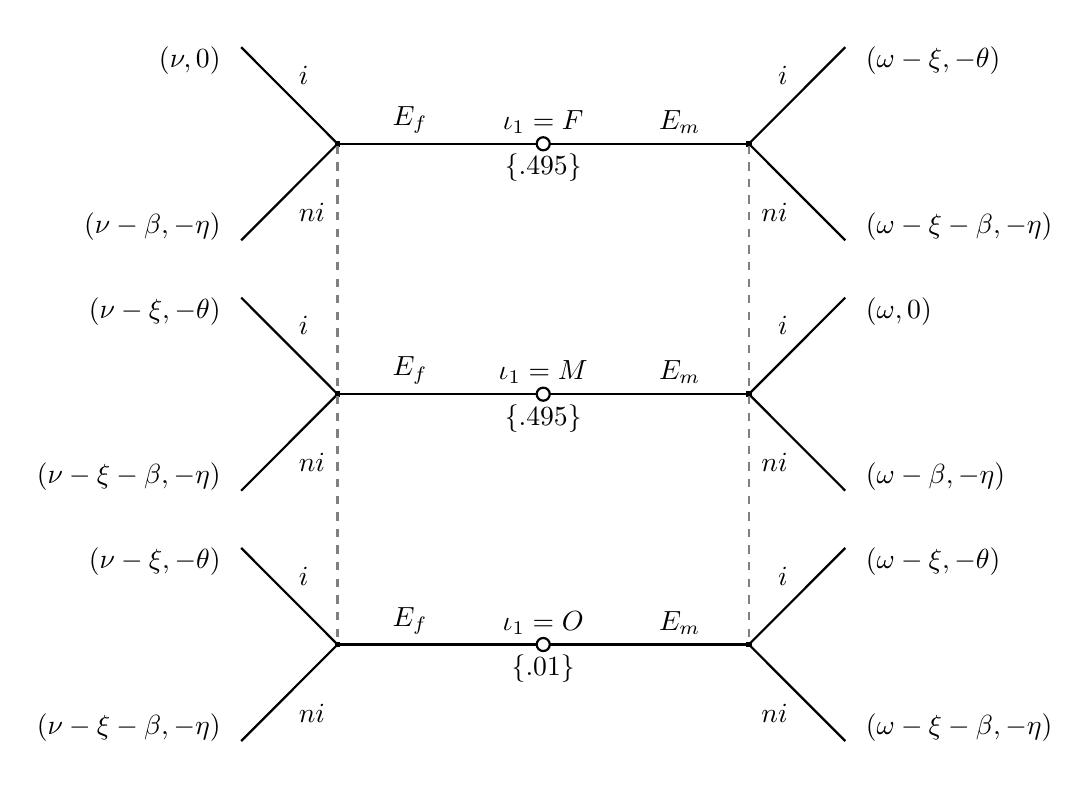
\begin{tikzpicture}[-,auto,node distance=3cm,thick,
	main node/.style={fill=black, scale=0.1, draw,font=\sffamily\small\bfseries},
	sub node/.style={font=\sffamily\small\bfseries}, 
	primer node/.style={circle,draw, scale=0.5, font=\sffamily\small\bfseries}]
	
	\node[primer node](F){};
		\node[above] at (F){$\iota_1=F$};
		\node[below] at (F){$\{.495\}$};
	\node[main node](F1)[left = 2.5 cm of F]{1};
		\node[sub node](FNC1)[above left = 1.7 cm of F1]{};
			\node[below left] at (FNC1){$(\nu,0)$};
		\node[sub node](FC1)[below left = 1.7 cm of F1]{};
			\node[above left] at (FC1){$(\nu-\beta, -\eta)$};	
	\node[main node](F2)[right = 2.5 cm of F]{1};
		\node[sub node](FNC2)[above right = 1.7 cm of F2]{};
			\node[below right] at (FNC2) {$( \omega-\xi,-\theta)$};
		\node[sub node](FC2)[below right = 1.7 cm of F2]{};
			\node[above right] at (FC2) {$(\omega-\xi-\beta,-\eta)$};	

	\node[primer node](M)[below = 3 cm of F]{};
		\node[above] at (M){$\iota_1=M$};
		\node[below] at (M){$\{.495\}$};
	\node[main node](M1)[left = 2.5 cm of M]{1};
		\node[sub node](MNC1)[above left = 1.7 cm of M1]{};
			\node[below left] at (MNC1){$(\nu-\xi, -\theta)$};
		\node[sub node](MC1)[below left = 1.7 cm of M1]{};
			\node[above left] at (MC1){$(\nu-\xi- \beta,-\eta)$};
	\node[main node](M2)[right = 2.5 cm of M]{1};
		\node[sub node](MNC2)[above right = 1.7 cm of M2]{};
			\node[below right] at (MNC2){$(\omega,0)$};
		\node[sub node](MC2)[below right = 1.7 cm of M2]{};
			\node[above right] at (MC2) {$(\omega-\beta,-\eta)$};
		
	\node[primer node](O)[below = 3 cm of M]{};
		\node[above]at (O){$\iota_1=O$};
		\node[below]at (O){$\{.01\}$};
	\node[main node](O1)[left = 2.5 cm of O]{1};
		\node[sub node](ONC1)[above left = 1.7 cm of O1]{};
			\node[below left] at (ONC1) {$(\nu-\xi,-\theta)$};
		\node[sub node](OC1)[below left = 1.7 cm of O1]{};
			\node[above left] at (OC1) {$(\nu-\xi-\beta,-\eta)$};
	\node[main node](O2)[right = 2.5 cm of O]{1};
		\node[sub node](ONC2)[above right = 1.7 cm of O2]{};
			\node[below right] at (ONC2){$( \omega -\xi,-\theta)$};
		\node[sub node](OC2)[below right = 1.7 cm of O2]{};
			\node[above right] at (OC2) {$(\omega-\xi- \beta, -\eta)$};
		
	\path[thick]
	(F)  edge node [above left]{$E_f$}(F1)
		 edge node [above right]{$E_m$}(F2)
	(F1) edge node [above right]{$i$}(FNC1)
		 edge node [below right]{$ni$}(FC1)
	(F2) edge node [above left]{$i$}(FNC2)
		 edge node [below left]{$ni$}(FC2)	 
	(M)  edge node [above left]{$E_f$}(M1)
		 edge node [above right]{$E_m$}(M2)
	(M1) edge node [above right]{$i$}(MNC1)
		 edge node [below right]{$ni$}(MC1)
	(M2) edge node [above left]{$i$}(MNC2)
	 	 edge node [below left]{$ni$}(MC2)			
	(O)  edge node [above left]{$E_f$}(O1)
		 edge node [above right]{$E_m$}(O2)
	(O1) edge node [above right]{$i$}(ONC1)
		 edge node [below right]{$ni$}(OC1)
	(O2) edge node [above left]{$i$}(ONC2)
		 edge node [below left]{$ni$}(OC2);
		 
	\draw[gray, dashed](F1)--(M1);
	\draw[gray, dashed](M1)--(O1);
	\draw[gray, dashed](F2)--(M2);
	\draw[gray, dashed](M2)--(O2);  	 	
	\end{tikzpicture}
	\begin{singlespace}
          \floatfoot{\footnotesize{\textbf{Nota:} Esta figura representa un juego de información imperfecta en el que el jugador 1 puede ser de identidad $\{ F, M,O \}$. Ese jugador puede tomar una acción que es expresión de género femenina $(E_f)$ o masculina $(E_m)$. El jugador 2 al observar una expresión de género, forma creencias sobre la identidad del jugador 1 y decide si interactúa $(i)$ o no interactúa $(ni)$ con este. En ausencia de normas sociales, $\nu$ es la utilidad de tomar una expresión de femenina y $\omega$ es la utilidad de tomar una expresión masculina. Si el jugador 1 rompe la norma social, percibe una desutilidad de $\xi$, y si interatúa con el jugador 2, le genera al jugador 2 una  externalidad de $\theta$. Si el jugador 2 decide no interactuar, percibe un costo de $\eta$ y le genera una externalidad al jugador 1 de $\beta$. }\par}
\end{singlespace}
\end{figure}

Al inicio del juego, el jugador 1 conoce su identidad y decide si tiene una expresión femenina o una masculina. El jugador 2 al observar la expresión de género del jugador 1, forma unas creencias sobre la identidad del jugador 1 y decide si interactúa o no. Los equilibrios bayesianos de Nash de este juego dependen de: (i) la utilidad relativa que le genera al jugador 1, dada su identidad, tener una expresión femenina frente a una expresión masculina (incorporando que el jugador 2 podría decidir no interactuar con él); y de (ii) la relación entre el costo de no interactuar y el costo esperado de observar que se viola la prescripción social. 

Existen seis posibles equilibrios bayesianos de Nash, cuatro agrupadores y dos separadores\footnote{Un equilibrio es agrupador cuando independiente de la identidad, el jugador 1 toma la misma acción y un equilibrio es separador cuando la acción que toma el jugador 1 depende de su identidad.}, que dependen de los parámetros poblacionales. Debido a que en los datos no se observan equilibrios agrupadores, esta sección expondrá únicamente los separadores.\footnote{El apéndice A expone los equilibrios agrupadores. El proceso de solución del modelo está disponible por solicitud.}

Existen equilibrios separadores, en estrategias puras, solo si las personas de identidad binaria cumplen la norma social. Es decir, el juego puede llegar a un equilibrio cuando el jugador 1 de identidad femenina (masculina) toma una expresión femenina (masculina). Bajo esa estrategia del jugador 1, el jugador 2 se enfrenta a dos posibilidades: (i) observa una expresión de género $E_k$ que toma el jugador 1 de una identidad binaria $(K)$ y el de identidad no binaria $(O)$, u (ii) observa una expresión de género $(E_{-k}$) que solo toma el jugador 1 de la otra identidad binaria $(-K)$, donde $K \in \{F,M\}$. Para ambos casos, la mejor respuesta del jugador 2 es no interactuar solo si el costo de no interactuar es menor al costo esperado de que se viole la norma social; de lo contrario, es mejor respuesta interactuar. El costo esperado de que el jugador 1 viole la norma social es el costo real de ver que viola la norma social $(\theta)$ ponderado por la creencia de que el jugador 1 está violando la norma social. Para los equilibrios separadores, como solo si el jugador 1 es de identidad no binaria se viola la norma social, el costo esperado de que se viole la norma social es $\theta^e=\theta*P(O|E_k)$, donde $P(O|E_k)$ es la creencia del jugador 2 de que el jugador 1 sea de identidad no binaria dado que observa la expresión de género que ese jugador toma. 

Además de las condiciones anteriores, para que exista equilibrio existen unos rangos en los que debe estar $\Pi(E_{-k})$  en relación con $\Pi(E_k)$, los costos que percibe el jugador 1 de no interactuar ($\beta$) y de actuar contrario a la norma social ($\xi$). Estos equilibrios son simétricos y están representados en la Figura \ref{fig:equilibrios}.

\begin{figure}[!ht]
\caption{Equilibrios separadores}
\hspace*{-2cm}
\begin{minipage}{0.4\textwidth}
    \centering
    Si $\xi > \beta$
    
    \footnotesize{
    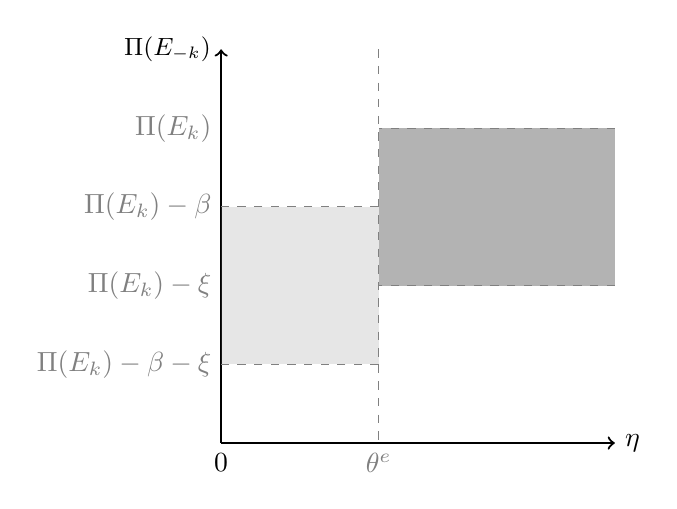
\begin{tikzpicture}
         \draw[black, thick][->] (0,0) -- (5,0) node[right] {$\eta$};
         \draw[black, thick][->] (0,0) node[below]{0} -- (0,5) node[left] {\small{$\Pi(E_{-k})$}};
         \draw[gray, dashed] (2,5) -- (2,0) node[below] {$\theta^e$};
         \draw[gray, dashed] (2,1) -- (0,1) node[left] {$\Pi(E_k)-\beta-\xi$};
         \draw[gray, dashed] (5,2) -- (2,2);
         \draw[gray, dashed] (2,3) -- (0,3) node[left] {$\Pi(E_k)-\beta$};
         \draw[gray, dashed] (5,4) -- (2,4) ;
         \draw[gray] (0,2) node[left] {$\Pi(E_k)-\xi$};
         \draw[gray] (0,4) node[left] {$\Pi(E_k)$};
         \draw[draw=gray, draw opacity=0, fill=gray, fill opacity=0.2] (2,1)--(0,1)--(0,3)--(2,3) -- cycle;
         \draw[draw=gray, draw opacity=0, fill=gray, fill opacity=0.6] (2,2)--(5,2)--(5,4)--(2,4) -- cycle;
    \end{tikzpicture}}
\end{minipage}
\hspace*{0.08\textwidth}
\begin{minipage}{0.4\textwidth}
\centering
Si $\beta > \xi$

\footnotesize{
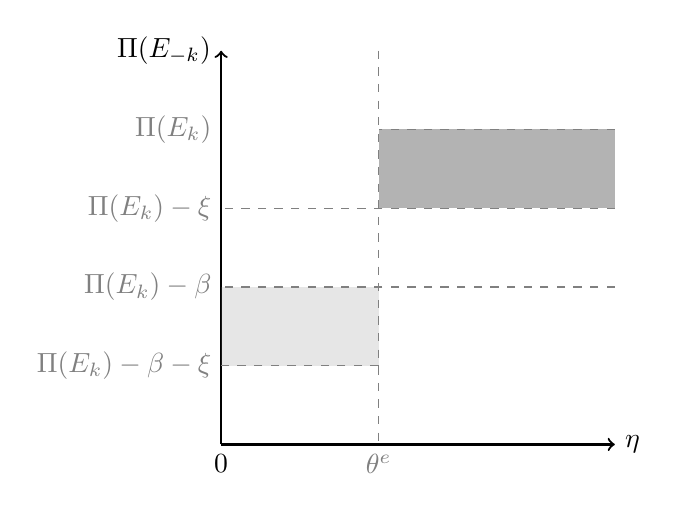
\begin{tikzpicture}
     \draw[black, thick][->] (0,0) -- (5,0) node[right] {${\eta}$};
     \draw[black, thick][->] (0,0) node[below]{0} -- (0,5) node[left] {$\Pi(E_{-k})$};
     \draw[gray, dashed] (2,5) -- (2,0) node[below] {$\theta^e$};
     \draw[gray, dashed] (2,1) -- (0,1) node[left] {$\Pi(E_k)-\beta-\xi$};
     \draw[gray, dashed] (5,2) -- (0,2) node[left] {$\Pi(E_k)-\beta$};
     \draw[gray, dashed] (5,3) -- (0,3) node[left] {$\Pi(E_k)-\xi$};
     \draw[gray, dashed] (5,4) -- (2,4) ;
     \draw[gray] (0,4) node[left] {$\Pi(E_k)$};
     \draw[draw=gray, draw opacity=0, fill=gray, fill opacity=0.2] (2,1)--(0,1)--(0,2)--(2,2) -- cycle;
     \draw[draw=gray, draw opacity=0, fill=gray, fill opacity=0.6] (2,3)--(5,3)--(5,4)--(2,4) -- cycle;
\end{tikzpicture}}
\end{minipage}
\label{fig:equilibrios}
\begin{minipage}{\textwidth}
    \centering
    \vspace*{0.5cm}
    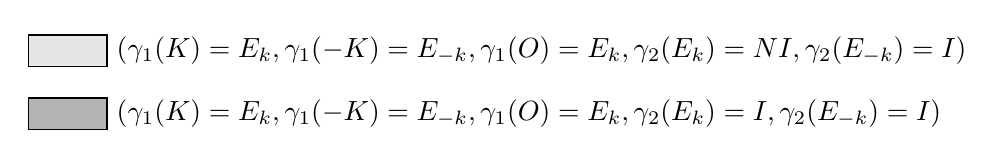
\begin{tikzpicture}
         \draw[draw=black, draw opacity=1, fill=gray, fill opacity=0.2] (1,0.8)--(0,0.8)--(0,1.2)--(1,1.2) -- cycle;
         \draw[black] (1,1) node[right] {$(\gamma_1(K)=E_k, \gamma_1(-K)=E_{-k}, \gamma_1(O)=E_k, \gamma_2(E_k)=NI, \gamma_2(E_{-k})=I)$};
         
         \draw[draw=black, draw opacity=1, fill=gray, fill opacity=0.6] (1,0)--(0,0)--(0,0.4)--(1,0.4) -- cycle;
         \draw[black] (1,0.2) node[right] {$(\gamma_1(K)=E_k, \gamma_1(-K)=E_{-k}, \gamma_1(O)=E_k, \gamma_2(E_k)=I, \gamma_2(E_{-k})=I)$};
         
    \end{tikzpicture}
\end{minipage}
%\begin{singlespace}
    %\floatfoot{\footnotesize{\textbf{Nota:} El área gris clara corresponde a los rango de los parámetros para los cuales el equilibrio es que el jugador 2 no interactúe cuando observa la expresión de género que toma el jugador 1 de identidad otra. El área gris oscura corresponde a los rango de los parámetros para los cuales el jugador 2 interactúa siempre.}\par}
%\end{singlespace}
\end{figure}
\vspace*{0.5cm}
\vfill
\begin{framed}
\noindent Sea $\gamma_i$ la estrategia del jugador $i$, y  sea $k \in \{F,M\}$,

\noindent (i) $(\gamma_1(K)=E_k, \gamma_1(-K)=E_{-k}, \gamma_1(O)=E_k, \gamma_2(E_k)=NI, \gamma_2(E_{-k})=I)$ es equilibrio si $\eta\in(0, \theta^e) \wedge \Pi_1(E_{k})- \beta \geq \Pi_1(E_{-k}) \geq  \Pi_1(E_{k})- \beta - \xi$

\noindent (ii) $(\gamma_1(K)=E_k, \gamma_1(-K)=E_{-k}, \gamma_1(O)=E_k, \gamma_2(E_k)=I, \gamma_2(E_{-k})=I)$ es equilibrio si $\eta\in[\theta^e, \infty) \wedge \Pi_1(E_{k}) \geq \Pi_1(E_{-k}) \geq \Pi_1(E_{k})- \xi$
\end{framed}

En resumen, la primera condición para que los jugadores lleguen a un equilibrio separador es que las personas de identidad binaria se adhieran a la norma social. Si esa condición se cumple, el equilibrio puede ser de dos tipos. El primer equilibrio sucede si el costo esperado de ver que se está violando la norma social es mayor al costo de no interactuar. En ese caso el jugador 2 solo interactúa con el jugador 1 si este le manda una señal que le de certeza de cuál es su identidad de género. El segundo equilibrio sucede si el costo de no interactuar es mayor al costo esperado de ver que se viola la norma social. En ese caso, el jugador 2 interactúa con el jugador 1 sin importar si cree que está violando la norma social. Estas condiciones son contrastadas con el experimento que presenta la siguiente sección. 

%Dado que el equilibrio depende del valor que tomen los parámetros del modelo, a continuación se presenta la estática comparativa de estos parámetros para los equilibrios separadores.
%
%\textit{Si el costo que percibe el jugador 1 de no interactuar se hace más grande, mientras que el costo de violar uno mismo la norma social se hace más pequeño ($\beta \to \infty \wedge \xi \to 0 $)}. (i) Si el costo neto de no interactuar es menor que la creencia del jugador 2 de que el jugador 1 es de identidad otra dado que observa $E_k$ ($\frac{\eta}{\theta} < P(O|E_k)$), solo hay equilibrio si $\Pi(E_{-k}) \to - \infty$ en la misma velocidad a la que $\beta \to \infty$. (ii) Si el costo neto de no interactuar es menor que la creencia del jugador 2 de que el jugador 1 es de identidad otra dado que observa $E_k$ ($\frac{\eta}{\theta} \geq P(O|E_k)$),  solo hay equilibrio si la utilidad de una expresión de género femenina es igual a la utilidad de una expresión masculina ($\Pi(E_{k})=\Pi(E_{-k})$). 
%
%\textit{Si el costo que percibe el jugador 1 de no interactuar y el costo de violar uno mismo la norma social se hacen más grandes ($\beta \to \infty \wedge \xi \to \infty$)}. (i) Si el costo neto de no interactuar es menor que la creencia del jugador 2 de que el jugador 1 es de identidad otra dado que observa $E_k$ ($\frac{\eta}{\theta} < P(O|E_k)$),  solo hay equilibrio si $\Pi(E_{-k}) \to - \infty$. (ii) Si el costo neto de no interactuar es menor que la creencia del jugador 2 de que el jugador 1 es de identidad otra dado que observa $E_k$ ($\frac{\eta}{\theta} \geq P(O|E_k)$), hay equilibrio incluso cuando la diferencia entre $\Pi(E_k)$ y $\Pi(E_{-k})$ sea grande, solo si  $\Pi(E_{-k}) \leq \Pi(E_k)$. 
%
%\textit{Si el costo que percibe el jugador 1 de no interactuar se hace más pequeño, mientras que el costo de violar uno mismo la norma social se hace más grande ($\beta \to 0 \wedge \xi \to \infty $)}. Tanto si el costo neto de no interactuar es menor que la creencia del jugador 2 de que el jugador 1 es de identidad otra dado que observa $E_k$ , como si el mayor ($\frac{\eta}{\theta} \in  [0, \infty)$), hay equilibrio incluso cuando la diferencia entre $\Pi(E_k)$ y $\Pi(E_{-k})$ sea grande, siempre que $\Pi(E_{-k}) \leq \Pi(E_k)$. 
%
%\noindent \textit{Si el costo que percibe el jugador 1 de no interactuar y el costo de violar uno mismo la norma social se hacen más pequeños ($\beta \to 0 \wedge \xi \to 0$)}. Tanto si el costo neto de no interactuar es menor que la creencia del jugador 2 de que el jugador 1 es de identidad otra dado que observa $E_k$, como si es mayor ($\frac{\eta}{\theta} \in  [0, \infty)$), solo hay equilibrio si la utilidad de una expresión de género femenina es igual a la utilidad de una expresión masculina ($\Pi(E_{k})=\Pi(E_{-k})$). 
%
%\noindent \textit{Si el costo que percibe el jugador 2 no interactuar se hace más grande o el costo de ver que se otro viole la norma social se hace más pequeño ($\eta \to \infty \vee \theta \to 0$)}. Es mejor respuesta del jugador 2 interactuar ante cualquier acción del jugador 1. Es decir, interactuar a pesar de no tener certeza de la identidad del jugador 1.
%
%\noindent \textit{Si el costo que percibe el jugador 2 no interactuar se hace más grande o el costo de ver que se otro viole la norma social se hace más pequeño ($\eta \to 0 \vee \theta \to \infty$)}. Es mejor respuesta del jugador 2 no interactuar cuando observa $E_k$, la acción que toma el jugador 1 de identidad otra, e interactuar cuando observa $E_{-k}$. Es decir, interactuar solo cuando tener certeza de la identidad del jugador 1 y no interactuar cuando la expresión de género que observa no le da certeza de la identidad del jugador 1. 
%
%La siguiente Sección presenta el experimento de este estudio, que sigue el juego anterior.
\section{El experimento}
Para el experimento, los estudiantes de pregrado de una universidad privada de Bogotá fueron invitados a participar en un concurso en el que debían hacer una tarea corta y sencilla. Esa tarea debían presentarla en grupos de tres personas. Estos estudiantes con frecuencia enfrentan procesos similares en los que deben formar un grupo para producir un contenido. Por lo tanto, las decisiones que tomaron en el experimento eran cercanas a su cotidianidad. 

El objeto de estudio de este trabajo son las preferencias de los estudiantes para elegir con quién hacer la tarea dado que, cuando hacen la elección, únicamente observaban unas características generales y una serie de expresiones de género de sus pares.  Los participantes tomaron todas las decisiones en línea por lo que no hubo ningún tipo de interacción entre los participantes previo a la toma de decisiones.\footnote{El experimento fue desarrollado en Otree \citep{otree}. El protocolo experimental está disponible por solicitud}.

Primero, los estudiantes se inscribieron a participar en el concurso. El formulario de inscripción incluía la explicación de cada paso del concurso y las fechas de estos. Las instrucciones fueron dadas siempre en el marco del concurso sin revelar cuáles eran las decisiones objeto de estudio. Los participantes quedaban inscritos solo si completaban el formulario de inscripción (encuesta de entrada). El propósito de esta encuesta era recoger información general de los participantes e identificar las expresiones de género relevantes para este estudio. Las inscripciones estuvieron abiertas dos semanas.

Luego, los participantes fueron asignados aleatoriamente a una sección de nueve personas. Las secciones fueron aleatorizadas para asegurar balance en el género de los participantes y en las características con las que iban a ser descritos cuando sus pares eligieran el grupo. Una vez fueron asignados a las secciones, cada participante recibió un enlace en el que observaba una tarjeta de descripción para cada una de las otras ocho personas de su sección. A partir de estas tarjetas, debían decidir con quién prefería desarrollar la tarea siguiendo un proceso de votación que está explicado más a adelante. 

El proceso de votación estuvo habilitado durante una semana. Luego de esto, los participantes fueron informados sobre quiénes estaban en su grupo. A partir de ese momento, tuvieron diez días para hacer la tarea, a pesar de que hacerla tomaba entre 5 y 30 minutos. Una semana después de que los grupos mandaran la tarea del concurso, un panel de jurados eligió los grupos ganadores. Fueron premiados siete grupos, el premio más alto fue de más del doble del salario mínimo diario (por persona del grupo) y el premio más bajo fue de un tercio del salario mínimo diario, lo equivalente a tres salarios mínimos por hora (por persona del grupo). Antes de recibir los premios los participantes respondieron una breve encuesta de salida.

\subsection{La formación de grupos}
Para el proceso de elección, cada participante observaba una tarjeta de caracterización para cada una de las otras ocho personas de su sección. A partir de esa caracterización, los participantes debían organizar los ocho perfiles en el orden en el que querían que esas personas hicieran parte de su grupo para hacer la tarea. Es decir, la persona con la que más querían hacer la tarea la debían poner el primer lugar; la segunda persona con la que más querían hacer la tarea la debían poner en el segundo lugar; así, hasta organizar los ocho perfiles. De manera que la persona con que menos querían hacer la tarea, la debían poner en el último lugar.

Todo esto se hizo a través de un enlace para asegurar que los participantes no pudieran ver a las otras personas de su sección y por lo tanto, no pudieran identificar de quién se trataba. Que la decisión la tomaran a través de un enlace que recibían por correo pudo generar que consultaran su decisión con otros participantes. Esto no invalida los resultados por dos razones. Primero, porque en la realidad cuando uno debe escoger con quién trabajar, en muchas ocasiones consulta esa decisión con otros. Segundo, las características en la tarjeta hacían imposible rastrear perfectamente quién era la persona asociada a esa caracterización.

Luego, los grupos fueron formados en tres pasos a partir de las listas que presentó cada participante. Primero, para cada sección, una de las nueve personas fue elegida aleatoriamente. El primer grupo de esa sección fue conformado por esa persona que se eligió aleatoriamente y las dos primeras personas en su lista. Segundo, de las seis personas que no fueron asignadas al primer grupo, una persona fue elegida aleatoriamente. El segundo grupo fue conformado por esa segunda persona elegida aleatoriamente y las dos primeras personas en su lista, que no fueron asignadas al primer grupo. El tercer grupo fue conformado por las tres personas que no fueron asignadas ni al primer ni al segundo grupo.

Se utilizó este proceso de formación de grupos, siguiendo a \cite{beautifulorwhite2012}, porque es compatible en incentivos. Más aún, porque el pago estaba completamente determinado por el desempeño en la tarea y el pago se hizo al grupo entero.

\subsection{Las tarjetas}
Las tarjetas que describían a cada participante tenían: (i) una imagen de la vestimenta que ese participante reconoció usaría con mayor frecuencia para ir a la universidad, (ii) la habilidad que reportó como más fuerte entre matemáticas y comunicación (habla, escucha, y escritura), (iii) la aspiración que reportó más fuerte para los próximos diez años entre estabilidad familiar y comodidad económica, (iv) la edad y (v) el departamento de nacimiento (ver Figura \ref{fig:tarjeta}). Cada participante reportó estas características entre una serie de preguntas en la encuesta de inscripción. Por lo tanto, a pesar de que al momento de inscribirse los participantes sabían que luego sus pares iban a observar una caracterización de ellos, la encuesta tenía suficientes preguntas para no poder identificar \textit{a priori} cuáles de sus respuestas iban a aparecer en la tarjeta. 

\begin{figure}[htbp]
	\centering
	\caption{Ejemplo de tarjeta de caracterización}
	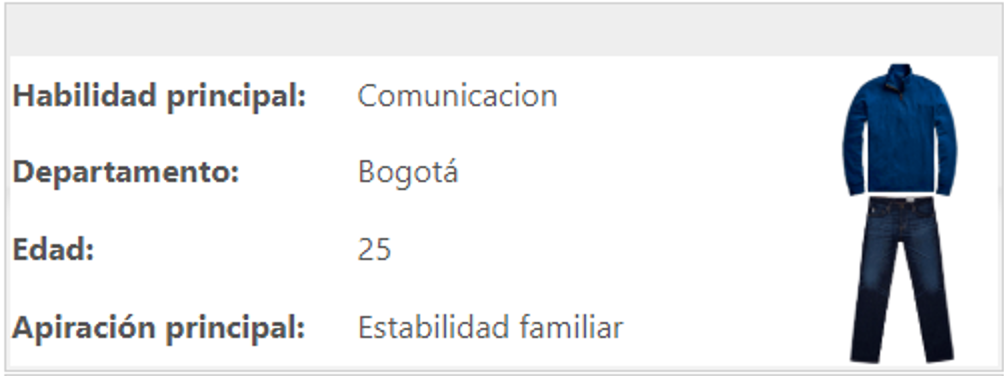
\includegraphics[width=7.7cm]{Images/tarjeta}
	\label{fig:tarjeta}
\end{figure}


\section{Los datos y las expresiones de género}
En el experimento se inscribieron 113 estudiantes de pregrado, de 29 de las 39 carreras de la universidad,\footnote{La participación por facultades se distribuye de la siguiente manera: 44\% de de Ingeniería, 13\% de Arquitectura y Diseño, 12\% de Ciencias Sociales, 10\% de Ciencias, 7\% de Arte y Humanidades, 6\% de Economía, 5\% de Derecho y 2\% de Administración y la Escuela de Gobierno.} de los cuales 56 se identificaron de manera masculina, 56 de manera femenina y uno se identificó de manera no binaria. A continuación, son descritos los criterios utilizados para clasificar la vestimenta, las habilidades y las aspiraciones como expresiones de género y se comprueba si, bajo esa clasificación, los participantes cumplen la norma social de que las personas de identidad femenina en promedio tienen expresiones femeninas y las personas de identidad masculina tienen expresiones masculinas. Lo anterior es una aproximación a si los participantes perciben la vestimenta, la habilidad o la aspiración como expresiones de género o no.

\subsection{Vestimenta} La vestimenta es una expresión visual con una fuerte asociación al género. Para identificar una vestimenta que mejor se acercara a la expresión de género de la persona, cada participantes observaba en la encuesta nueva vestimentas (ver Figura \ref{fig:vestimentas}).\footnote{Estas imágenes aparecían en un orden aleatorio, diferente para cada participantes para evitar efectos de orden.} Los participantes debían elegir cuál de esas vestimentas usaría con mayor frecuencia para ir a la universidad.

\begin{figure}[htbp]
    \centering
    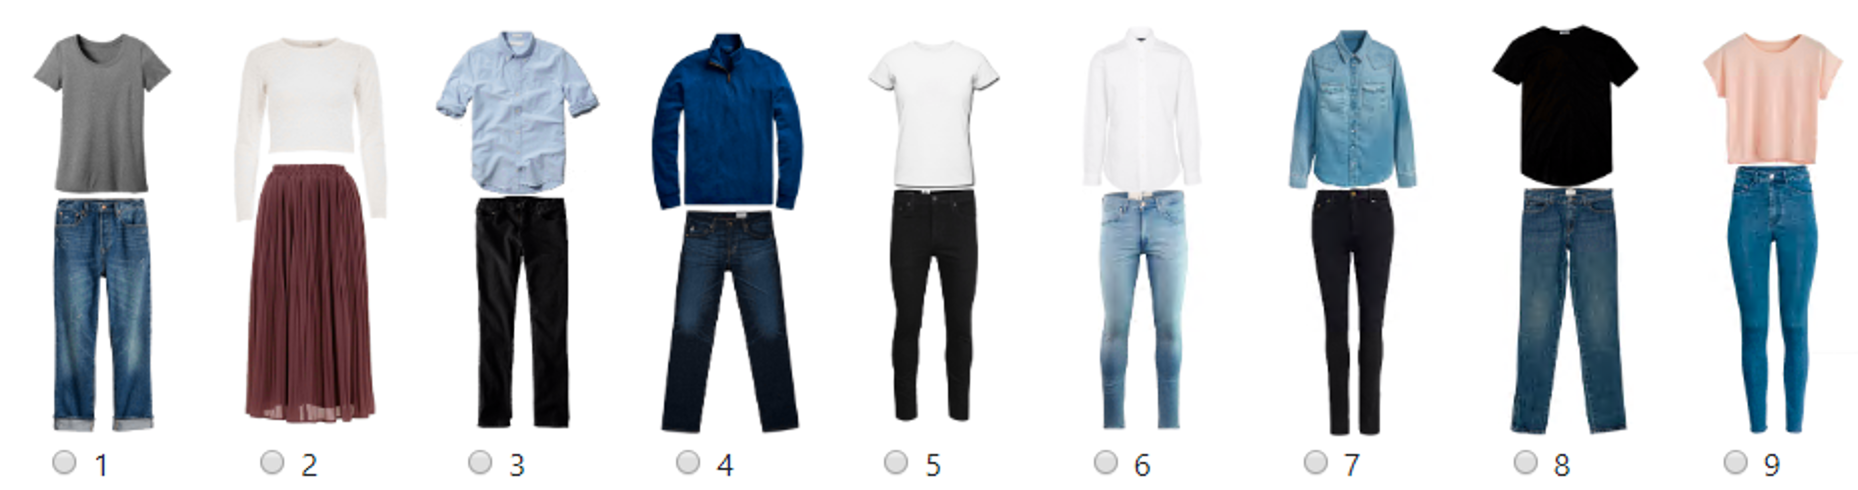
\includegraphics[width=14cm]{Images/vestimentas.png}
    \caption{Opciones de vestimentas a elegir}
    \label{fig:vestimentas}
    \begin{singlespace}
    \floatfoot{\footnotesize{\textit{Nota:} La figura contiene las opciones de vestimenta que observaban los participantes en la encuesta de inscripción. A cada persona le salía las vestimentas en un orden aleatorio y debían elegir la opción que consideraban usarían con mayor frecuencia para ir a la universidad.}\par}
    \end{singlespace}
\end{figure}

Las vestimentas fueron clasificadas como expresión de género masculina o femenina a partir de una encuesta de percepción hecha a una muestra de estudiantes diferente a la de los participantes, pero de la misma universidad. En esa encuesta, las personas debían responder de 1 a 9 qué tan masculina o femenina percibían esa vestimenta.\footnote{Para la mitad de los encuestados, 1 representaba muy femenina y para la otra mitad, 1 representaba muy masculina.} El puntaje promedio de cada vestimenta fue asignado a esta y luego, en la muestra de participantes, ese puntaje fue estandarizado. El puntaje estandarizado, que es creciente en la feminidad, es la medida de cada vestimenta como expresión de género. 

Entre los participantes, la elección de vestimentas es bimodal y está altamente relacionado con la identidad de género de los participantes (ver Figura \ref{fig:distribuciones_expresiones}; p-valor de la prueba Kolmogorov-Smirnov: 0.000). En promedio, el puntaje de la vestimenta que eligieron las personas de identidad masculina es de -0.81 (d.e 0.49) y el de las personas de identidad femenina es de 0.81 (d.e 0.64). Esto es indicativo de que los participantes sí perciben la vestimenta como expresión de género. 

\subsection{Habilidad} 
La habilidad es una aproximación a la norma social de que las mujeres son buenas comunicándose y los hombres son buenos para las matemáticas. Esta expresión de género es relevante en este caso dado que el experimento fue conducido en un ambiente universitario en el que existe una baja participación femenina en carreras intensivas en matemáticas y una baja participación masculina en carreras de ciencias sociales. Esta norma social y su persistencia a través de las generaciones ha sido ampliamente estudiado por la literatura \citep{nollenberger2016mathgap, giuliano2017gender, saltiel2019gendergapinSTEM, spencer1999mathgenderstereotype, cvencek2011mathgenderstereotype}.

\begin{figure}[htbp]
    \centering
    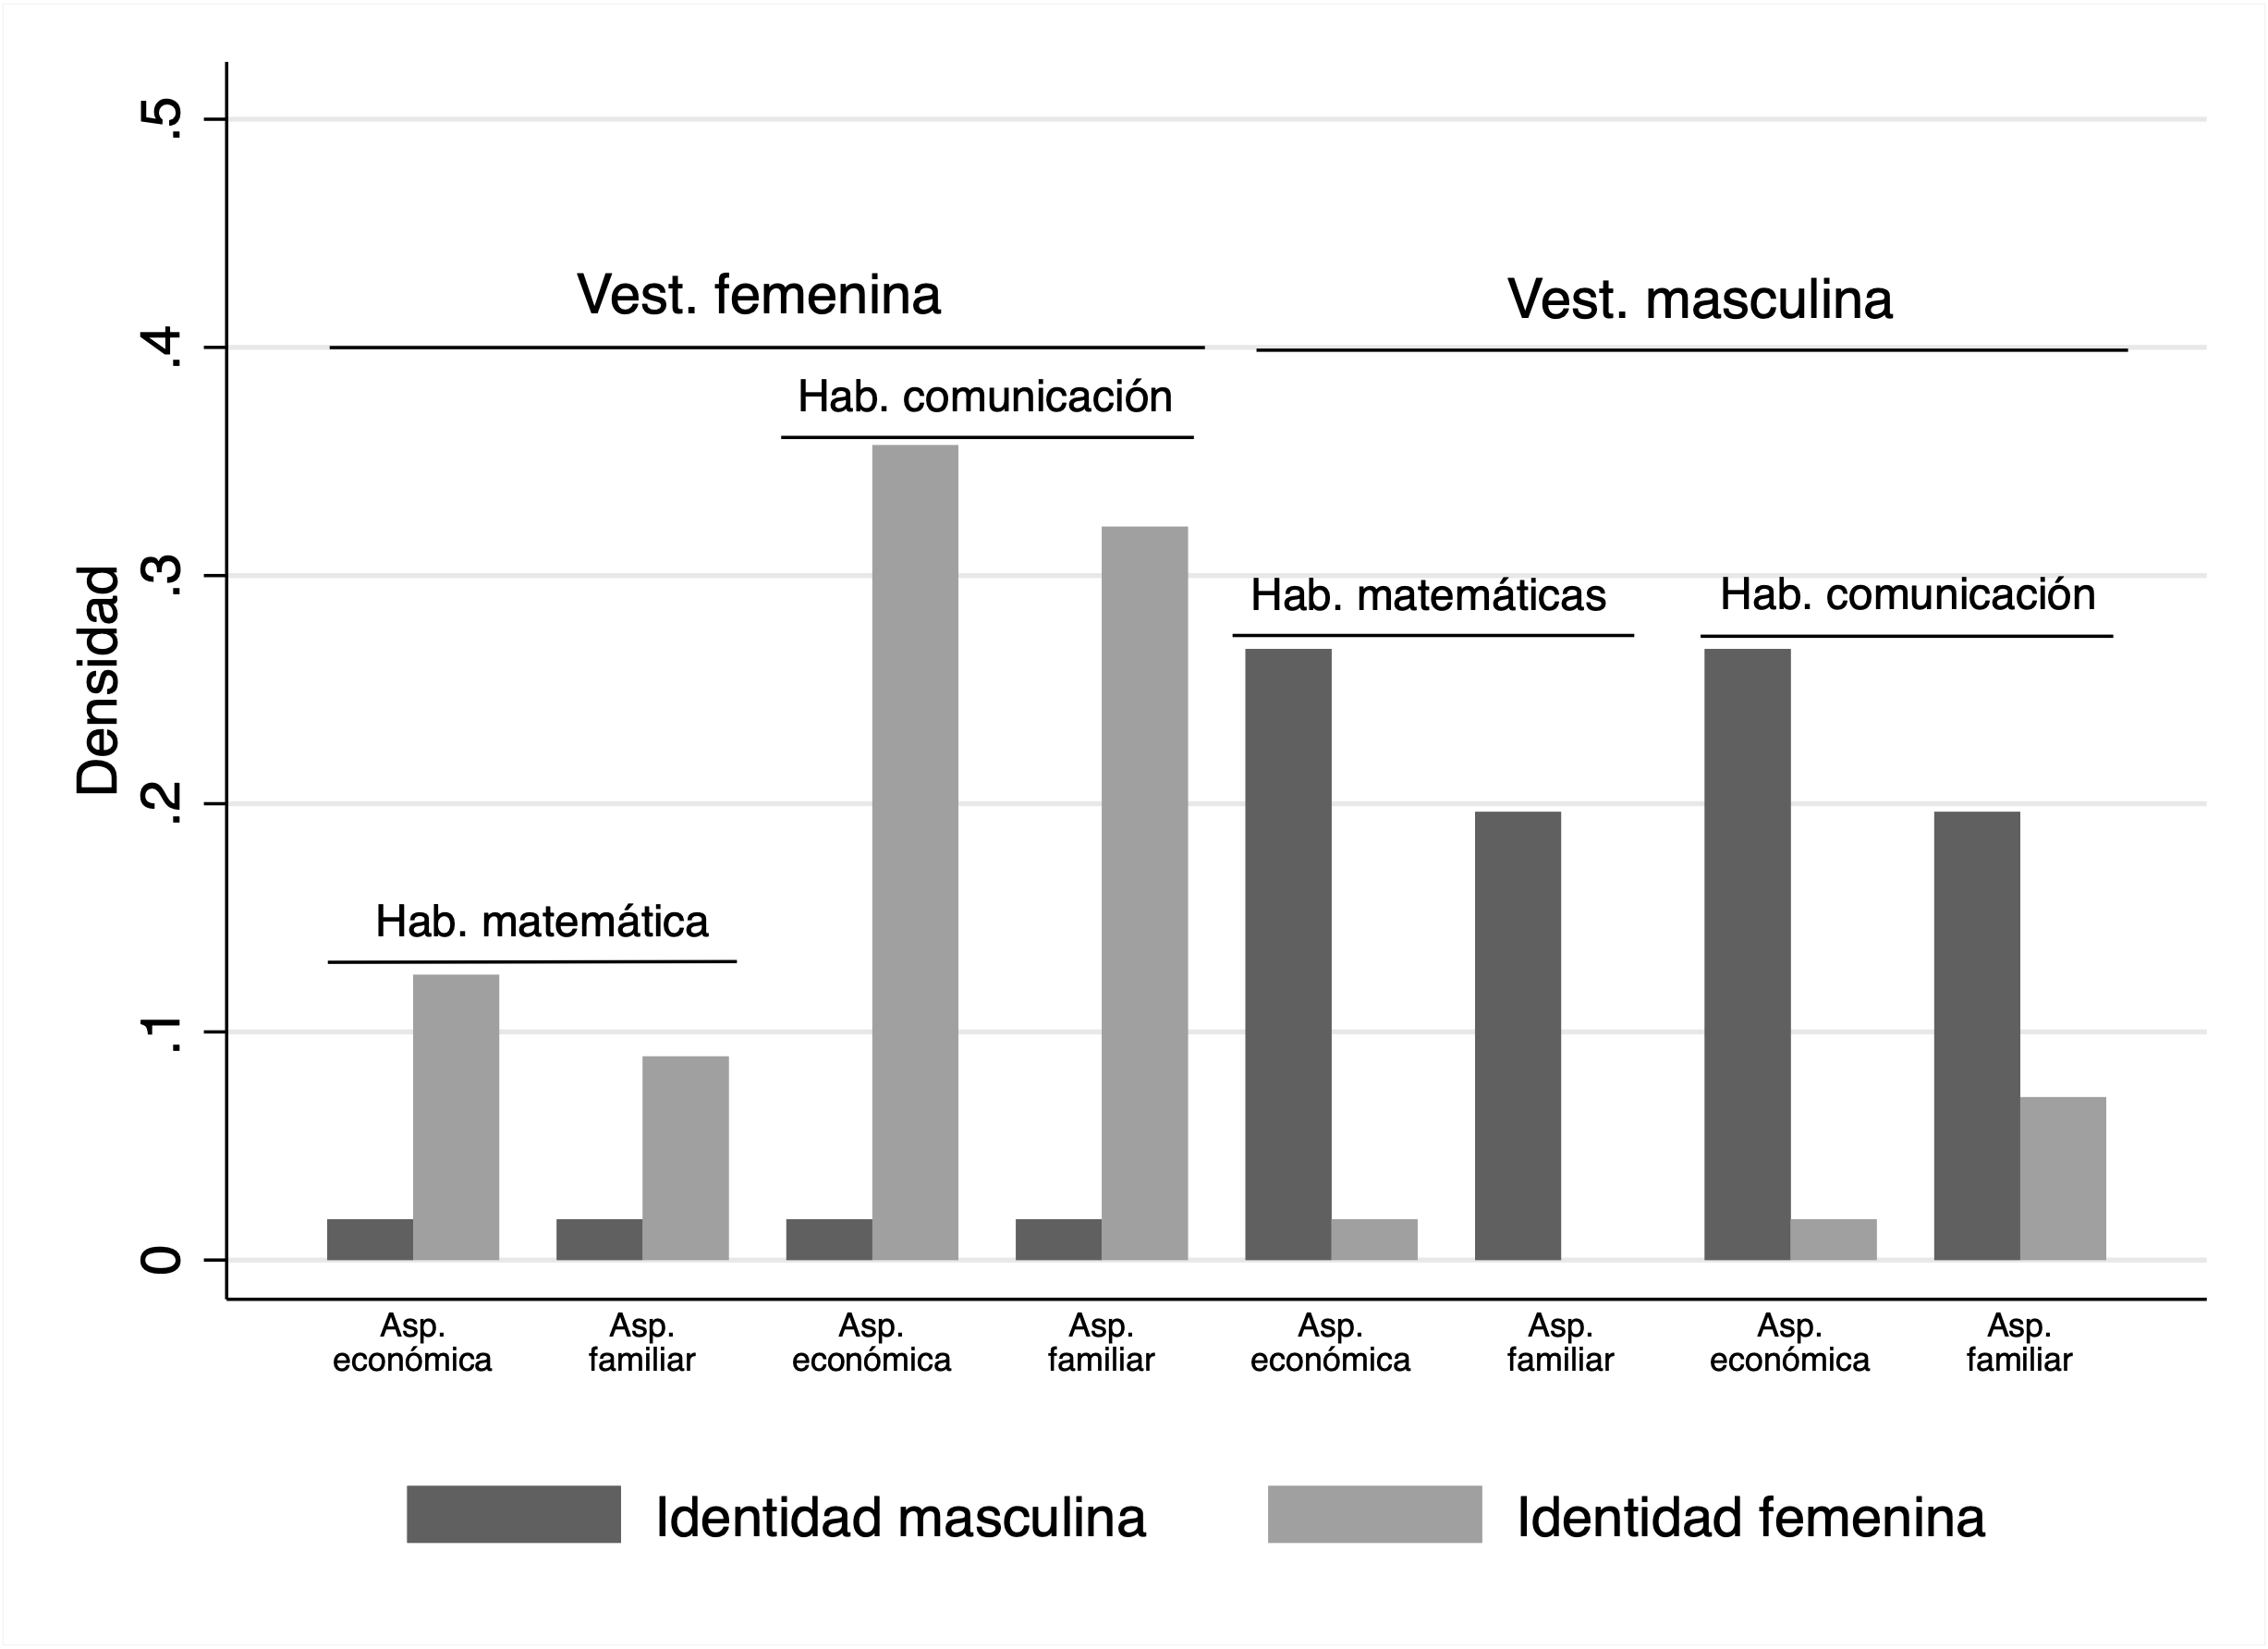
\includegraphics[width=11cm]{Images/dist.png}
    \caption{Distribución por género de vestimenta, habilidad y aspiración}
    \label{fig:distribuciones_expresiones}
    \begin{singlespace}
    \floatfoot{\footnotesize{\textit{Nota:} La figura representa la cantidad de participantes con esas características, discriminado por la identidad de género que reportó cada participante en la inscripción. Para esta gráfica, se definió una vestimenta femenina aquella que tenía un puntaje $>\ 0$ y una vestimenta masculina una con un puntaje $<\ 0$. El puntaje de la vestimenta es un puntaje estandarizado. La Tabla \ref{tab:distribuciones_expresiones} presenta esta información y contiene el número de observaciones por categoría.}\par}
    \end{singlespace}
\end{figure}

Además, en la encuesta de percepción hecha a una muestra diferente a la de los participantes, las personas respondieron de 1 a 9 qué tan masculina o femenina percibían 30 carreras universitarias. Al clasificar las carreras entre intensiva y no intensivas en matemáticas, la percepción de las personas que respondieron esta encuesta es que todas las carreras no intensivas en matemáticas son consideradas femeninas, en algún grado. Mientras que el 75\% de las carreras intensivas en matemática son consideradas masculinas. El 25\% de las carreras intensivas en matemáticas que no perciben masculinas, las perciben mínimamente femeninas -muy cerca al punto neutral- (ver Figura \ref{fig:careers}). Esta clasificación de las carreras valida la norma social que asocia las matemáticas con lo masculino y las comunicaciones con lo femenino.

Para identificar si los participantes creían ser más hábiles en matemáticas o en comunicación, la encuesta de entrada incluía una lista de ocho habilidades, entre las que estaban estas dos. Para cada habilidad, debían responder de 1 a 4 qué tan hábiles son. Luego debían responder con una escala de likert si consideraban ser mucho más hábiles en matemáticas o mucho más hábiles comunicándose. La encuesta incluía otra escala de likert, entre otras dos habilidades, para no hacer evidente cuáles eran las habilidades de interés. En la tarjeta, aparecía como habilidad principal comunicación (matemáticas) si le daban a esta un mayor puntaje que a matemáticas (comunicación). En caso de que le dieran el mismo puntaje, la habilidad principal era la que reportaran en la escala de likert como la más fuerte. Para aproximadamente el 97\% de la muestra, la habilidad definida con el puntaje es igual a la que reportaron en la escala de likert. 

Entre los participantes del experimento, existe una diferencia entre la habilidad que perciben más fuerte las personas femeninas que las masculinas (ver Figura \ref{fig:distribuciones_expresiones}; p-valor de prueba $\chi^2$: 0.003). Esta diferencia se debe a que el 76\% de las personas de identidad femenina considera ser mucho más hábiles comunicándose que en matemáticas. Mientras que las personas de identidad masculina se distribuyen en partes iguales entre aquellos que consideran ser más hábiles en matemáticas y los que consideran ser más hábiles comunicándose. Por lo que, al menos las personas de identidad femenina, sí perciben la habilidad como una expresión de género. 

\subsection{Aspiración principal} 
La aspiración principal busca identificar si en los próximos 10 años las personas aspiran más a tener una familia estable o tener mucha comodidad económica. La aspiración familiar es una aproximación a la norma social de que las mujeres se encargan del hogar y del cuidado de otros, mientras que los hombres son los proveedores económicos del hogar. Lo anterior siguiendo la literatura que ha estudiado la distribución de labores en el hogar, la carga de cuidado que asumen las mujeres \citep{floro1995gendertimeallocation, urdinola2017timeusegender}, la participación laboral en relación como la maternidad \citep{lundborg2017childrencareer}  y la distribución de ingresos al interior del hogar \citep{bertrand2015genderandincome, Robinson2012incomeallocationandshocks}, entre otros. 

Siguiendo la misma estructura utilizada para categorizar la habilidad principal,  los participantes debían responder para siete elementos, de 1 a 4,  qué tan importante es para ellos tener eso en los próximos 10 años. Entre esos siete elementos estaban estabilidad familiar y vivir muy cómodo económicamente. Luego debían responder dos escalas de likert sobre sus aspiraciones, una de ellas ponía en un extremo la comodidad económica y en el otro extremo la estabilidad familiar. En la tarjeta que caracterizaba a una persona aparecía una aspiración familiar (económica) si reportaba que era más importante en los próximos 10 años tener estabilidad familiar (comodidad económica) que comodidad económica (estabilidad familiar). En caso de que le dieran el mismo puntaje, la aspiración que aparecía en la tarjeta era la que reportaron que aspiran más en la escala de likert. Al igual que con la habilidad, en la mayoría de los casos la aspiración construida con la relación entre el puntaje que le dio a la estabilidad familiar y a la comodidad económica, coincidía con lo que reportó en la escala de likert. 

Entre los participantes no existe una diferencia clara entre la frecuencia de personas de identidad femenina y las de identidad masculina que aspiran más a tener estabilidad familiar ni las que aspiran más a tener comodidad económica (ver Tabla ver Figura \ref{fig:distribuciones_expresiones};  p-valor de la prueba $\chi^2$: 0.569). Esto es indicativo de que, para esta muestra, la aspiración no es percibida como una expresión de género. Por lo tanto, en adelante no se tomará en cuenta la aspiración como expresión de género. 

Existen varias posibilidades de por qué esta muestra no percibe la aspiración como expresión de género. Primero, puede existir un cambio generacional y diferencias contextuales. La literatura ha estudiado la división de trabajo en el hogar para una generación y un contexto diferente. Por lo que es posible, que la asociación familia- femenino, trabajo/recursos económicos-masculino se haya perdido. Segundo, puede que la asociación siga existiendo, pero no a nivel de aspiraciones. Es decir, una persona puede reconocer que la sociedad espera una mujer cuidadora y un hombre proveedor, pero que su aspiración sea ir más allá de lo que la sociedad espera. 


\section{Hipótesis y resultados}
Dado que la norma social se cumple, al menos para la vestimenta y las habilidades, esta sección estudia cómo responden los participantes al observar diferentes combinaciones de expresiones de género en su pares.

\subsection{Hipótesis}
\begin{hyp}
Cuando una persona no cumple la norma social o no es claro que la cumpla, la disposición a interactuar con esa persona es menor a si sí cumpliera la norma social. 
\end{hyp}

Dado que, en promedio, sí se cumple que las personas de identidad binaria se adhieran a la norma social, la primera predicción es que cuando las expresiones de género no señalizan claramente la identidad de género, la disposición a interactuar con esa persona va a ser más baja que si sus expresiones señalizaran claramente la identidad. Es decir, si una persona tiene una expresión de género femenina y otra masculina, la disposición de otros a interactuar con esa persona va a ser más baja a que si todas sus expresiones fueran femeninas o todas masculinas. Esta hipótesis sugiere que el costo de no interactuar es menor al costo esperado de que la persona esté violando la norma social ($\mathbb{P}$). 

\begin{hyp}
Las normas sociales y la disposición a interactuar varía entre identidades de género.
\end{hyp}

La literatura no ha explorado cómo el género de las personas se correlaciona con cómo responden a las normas sociales al momento de decidir interactuar con otros. Sin embargo, sí ha estudiado diferencias de comportamiento entre sexos en el juego del ultimátum (negociación), aunque los efectos que han encontrado son mixtos \citep{solnick2001genderultimatumgame, eckel2001chivalryultimatumgame, gomez2018gendernegociacion}.\footnote{\cite{solnick2001genderultimatumgame} encuentran que los hombres atraen mayores ofertas; mientras \cite{eckel2001chivalryultimatumgame} y \cite{gomez2018gendernegociacion} no encuentran diferencias en las ofertas. \cite{solnick2001genderultimatumgame} y \cite{gomez2018gendernegociacion} encuentran que los hombres rechazan más las ofertas de los hombres; mientras que \cite{eckel2001chivalryultimatumgame} encuentra que los hombres aceptan más las ofertas de las mujeres.} 

A pesar de que en el modelo las normas sociales son percibidas de igual manera por todos los jugadores, independiente de su identidad, la siguiente predicción es que la manera en que responden a las normas sociales varia entre géneros. Esto es que el costo de ver que se viola la norma social ($\theta$) es diferente entre identidades de género para cada combinación de expresiones de género que observe. Es decir el costo que percibe una persona de identidad femenina de ver que una persona de identidad masculina rompe la norma social es diferente al de ver a una persona de identidad no binaria romper la norma social. Estos, a su vez son diferentes a los costos que percibe una persona de identidad masculina o de identidad no binaria. Dados los límites de la literatura y del modelo, 
esta hipótesis se limita a esperar diferencias en la magnitud en la que responden personas de diferentes identidades al momento de elegir con quién interactuar. 

\begin{hyp}
Las personas que se adhieren a la norma social están menos dispuestas a interactuar con las personas que no cumplan la norma social. 
\end{hyp}

En el modelo, el jugador con identidad percibe el costo de violar la norma social, mientras que el otro jugador percibe el costo de interactuar con alguien que viola la norma social. Por el contrario, en el experimento los participantes enfrentaban ambos costos. La tercera predicción es que aquellas personas que cumplen la norma social están menos dispuestas a interactuar con una persona que señaliza estar violando la norma social. Esto es que si una persona percibe un costo alto de violar la norma social ($\xi$), también percibe un costo alto de interactuar con alguien que viola la norma social ($\theta$). Esto no quiere decir que todas las personas que se adhieren a la norma social lo hacen porque perciban un costo alto de violar la norma social, porque lo pueden hacer por la utilidad intrínseca que les genere esas expresiones; pero, sí supone que las personas que tienen un costo alto de violar la norma social, la cumplen.

\subsection{Estrategia empírica}
Para estimar cómo cambia la disposición a interactuar con una persona cuando cambia el conjunto de expresiones de género de esa persona, la información relevante es el orden que ocupó la persona $j$ cuando la persona $i$ organizó los perfiles y las características reportadas de la persona $j$.

Sea $Ranking_{ij}$ el orden inverso que la persona $i$ le asigna a la persona $j$, de manera que un valor más alto en \textit{Ranking} implica que la persona $i$ prefería trabajar con la persona $j$ por encima a las personas con menor \textit{Ranking} que $j$. Sea $vestimenta_j$ el puntaje estandarizado de qué tan femenina o masculina es la vestimenta que la persona $j$ eligió, donde un puntaje más alto implica que la vestimenta fue clasificada como más femenina. Sea $habilidad_j$ un indicador que toma el valor de uno si la  persona $j$ reporta ser más hábil comunicándose que en matemáticas. Sea $aspiracion_j$ un indicador que toma el valor de uno si la aspiración principal de la persona $j$ es familiar. Sean $edad_j$ la edad que reporta la persona $j$, $bogota_j$ un indicador de si la persona $j$ nació en Bogotá, $posicion\_inical_j$ el puesto que tenía la persona $j$ en la lista de la persona $i$ antes de que la persona $i$ reorganizara los perfiles según su preferencia y sea $\gamma_i$ el efecto fijo de la persona $i$; el modelo principal es: 
\begin{equation}
    \begin{split}
	Ranking_{ij}=& \beta_1vestimenta_j +  \beta_2habilidad_j + \beta_3habilidad_j\times vestimenta_{j} \\
	+ & \beta_4aspiracion_j + \beta_5edad_j + \beta_6bogota_j + \beta_7posicion\_inicial_j+\gamma_i + \epsilon_{ij}
	\end{split}
\end{equation}
Los resultados principales, basados en la estimación por MCO\footnote{El Apéndice C presenta las estimaciones por Logit rankeado y ordenado, y la estimación utilizando el \textit{ranking} promedio que recibió la persona $j$ entre todas las personas que observaron ese perfil.} de la Ecuación 1, consisten en las pruebas de hipótesis de si existe diferencia entre el \textit{ranking} esperado de una persona con todas sus expresiones masculinas (femeninas) con el \textit{ranking} esperado de cada una de las demás combinaciones de expresiones de género. Por ejemplo, una de las pruebas de hipótesis es si existe una diferencia entre el \textit{ranking} esperado de una persona con vestimenta femenina y que considera ser más hábil comunicándose (todas las expresiones femeninas) y el \textit{ranking} esperado de una persona con vestimenta femenina, que considera ser más hábil en matemáticas. Para las pruebas de hipótesis una vestimenta muy femenina (muy masculina) está definida como una vestimenta con un puntaje 1.5 desviaciones estándar arriba (abajo) de la media.

Para evaluar la Hipótesis 2, la Ecuación 1 fue estimada incluyendo la interacción del género de quien ordena los perfiles (la personas $i$, en adelante el \textit{ranker}) con las combinaciones de las expresiones de género. Luego, a partir de esa estimación, el \textit{ranking} que le da un \textit{ranker} femenino  a cada combinación de expresiones de género, es comparado con el que le da un \textit{ranker} masculino. También son comparados el \textit{ranking} esperado de una persona con todas sus expresiones femeninas (masculinas) con el \textit{ranking} esperado de las demás combinaciones de expresiones, cuando el \textit{ranker} es femenino y cuando es masculino. 

Para evaluar la Hipótesis 3, primero se definió que una persona cumplía la norma social (en adelante \textit{compliers}) si: (i) su identidad era masculina, había elegido una de las tres vestimentas más masculinas y consideraba ser más hábil en matemáticas, o  (ii) su identidad era femenina, había elegido una de las tres vestimentas más femeninas y consideraba ser más hábil comunicándose. Luego, la Ecuación 1 fue estimada incluyendo la interacción del indicador de \textit{complier} con las combinaciones de expresiones de género. Con base en esa estimación, el \textit{ranking}  que le da un \textit{complier} a cada combinación de expresiones de género es comparado con el que le da un no \textit{complier}. También son comparados el \textit{ranking} esperado de una persona que señaliza que cumple la norma social con el \textit{ranking} de las demás combinaciones de expresiones de género, cuando organiza los perfiles un \textit{complier} y cuando lo hace un no \textit{complier}. 

\subsection{Resultados}
Esta sección presenta los resultados del experimento. Estos resultados son sugestivos dado que para el tamaño de la muestra no hay poder para detectar resultados significativos.\footnote{El Apéndice D contiene los cálculos de poder.}

En la población agregada, una persona con todas sus expresiones de género femeninas recibe el mejor \textit{ranking}. En general, existe una preferencia por trabajar con las personas que reportan ser más hábiles comunicándose. Esta preferencia posiblemente se debe a que para el desarrollo de la tarea había un beneficio marginalmente mayor  de tener habilidades de comunicación. 

Lo que resulta interesante es que dentro de las personas cuya habilidad principal era la comunicación, las personas con una vestimenta femenina recibieron un \textit{ranking} 0.06d.e. más alto que las que tenían una vestimenta masculina. De manera similar, dentro de las personas que reportaron ser más hábiles en matemáticas, las personas que eligieron una vestimenta masculina, en promedio estuvieron 0.17d.e. más arriba en el \textit{ranking} que las personas con una vestimenta femenina. 

Por otra parte, en la población agregada, la diferencia entre el el \textit{ranking} que recibió una persona más hábil comunicándose y el \textit{ranking} que recibió una persona más hábil en matemáticas, aumenta a medida que la vestimenta es más femenina. Para una persona que eligió una vestimenta muy masculina, pasar de reportar como habilidad principal las matemáticas a reportar la comunicación aumentaba su \textit{ranking} en 0.1d.e. Mientras que para una persona con vestimenta muy femenina, pasar de reportar como habilidad principal las matemáticas a reporta la comunicación, aumenta su \textit{ranking} en 0.33d.e. 

\begin{table}[ht!]
    \centering
    \caption{Elección de pares a partir de expresiones de género}
    \label{tab:reg}
    \begin{threeparttable} \fontsize{8.5}{12}\selectfont {
    \begin{tabular}{lccccc} \hline \hline
                                                & \multicolumn{5}{c}{Ranker}                                                    \\\cmidrule{2-6}
                                                &   Todos   &  Femenino & Masculino & \textit{Complier} & No \textit{Complier}  \\ 
                                                &   (1)     &    (2)    &   (3)     &   (4)             & (5)                   \\ \hline
                                                &           &           &           &                   &                       \\
    Puntaje vestimenta                          &   -0.132  &   -0.344  &   0.035   &   -0.000	        &   -0.229              \\
                                                &   (0.207)	&   (0.312)	&   (0.280) &   (0.347)	        &   (0.266)             \\
    Habilidad comunicación                      &   0.497**	&   0.639*	&   0.322   &    0.286	        &   0.676**             \\
                                                &   (0.231)	&   (0.336)	&   (0.323) &   (0.372)	        &   (0.310)             \\
    Habilidad comunicación*Puntaje vestimenta   &   0.176	&   0.299	&   0.106   &    0.217	        &   0.153               \\
                                                &   (0.258)	&   (0.383)	&   (0.355) &   (0.414) 	    &   (0.351)             \\
    Aspiración familiar                         &   0.252	&   0.572*	&   -0.021  &    0.285	        &   0.225               \\
                                                &   (0.216)	&   (0.314)	&   (0.304) &   (0.301)	        &   (0.307)             \\
    Edad                                        &   0.001	&   -0.032	&   0.025   &    0.124	        &   -0.091              \\
                                                &   (0.064)	&   (0.091)	&   (0.093) &   (0.088)	        &   (0.091)             \\
    Bogotá = 1                                  &   -0.052	&   -0.160	&   0.023   &   -0.171	        &   0.125               \\
                                                &   (0.225)	&   (0.342)	&   (0.300) &   (0.314)	        &   (0.324)             \\
    Posición Inicial                            &  0.263***	&  0.263***	&  0.267*** &   0.368***    	&   0.178***            \\
                                                &   (0.046)	&   (0.066)	&   (0.065) &   (0.063)         &	(0.066)             \\
    Constante                                   &   2.873**	&   3.346*	&   2.564   &    0.107	        &   4.946**             \\
                                                &   (1.373)	&   (1.925)	&   (1.988) &   (1.895)	        &   (1.932)             \\
                                                &           &           &           &                   &                       \\
    Observaciones                               &   560     &   264     &   296     &   272             &   288                 \\
    Número de rankers                           &   70      &   33      &   37      &   34              &   36                  \\ \hline \hline
    \end{tabular}}
    \begin{tablenotes}
    \scriptsize{
    \item Nota: *** p$<$0.01, ** p$<$0.05, * p$<$0.1; errores estándar robustos en paréntesis.}
    \end{tablenotes}
    \end{threeparttable}
\end{table}

\begin{result}
Condicional en la habilidad, sugestivamente existe una mayor disposición a interactuar con las personas que señalizan que cumplen la norma social, especialmente cuando señaliza una identidad femenina. 
\end{result}

\begin{figure}[t!]
    \centering
    \label{fig:hypothesis_graphs}
    \caption{Ranking esperado por combinación de expresiones de género}
    \begin{minipage}{0.245\textwidth}
        
    \end{minipage}
    \begin{subfigure}{0.49\textwidth}
        \centering
        \caption{Todos}
        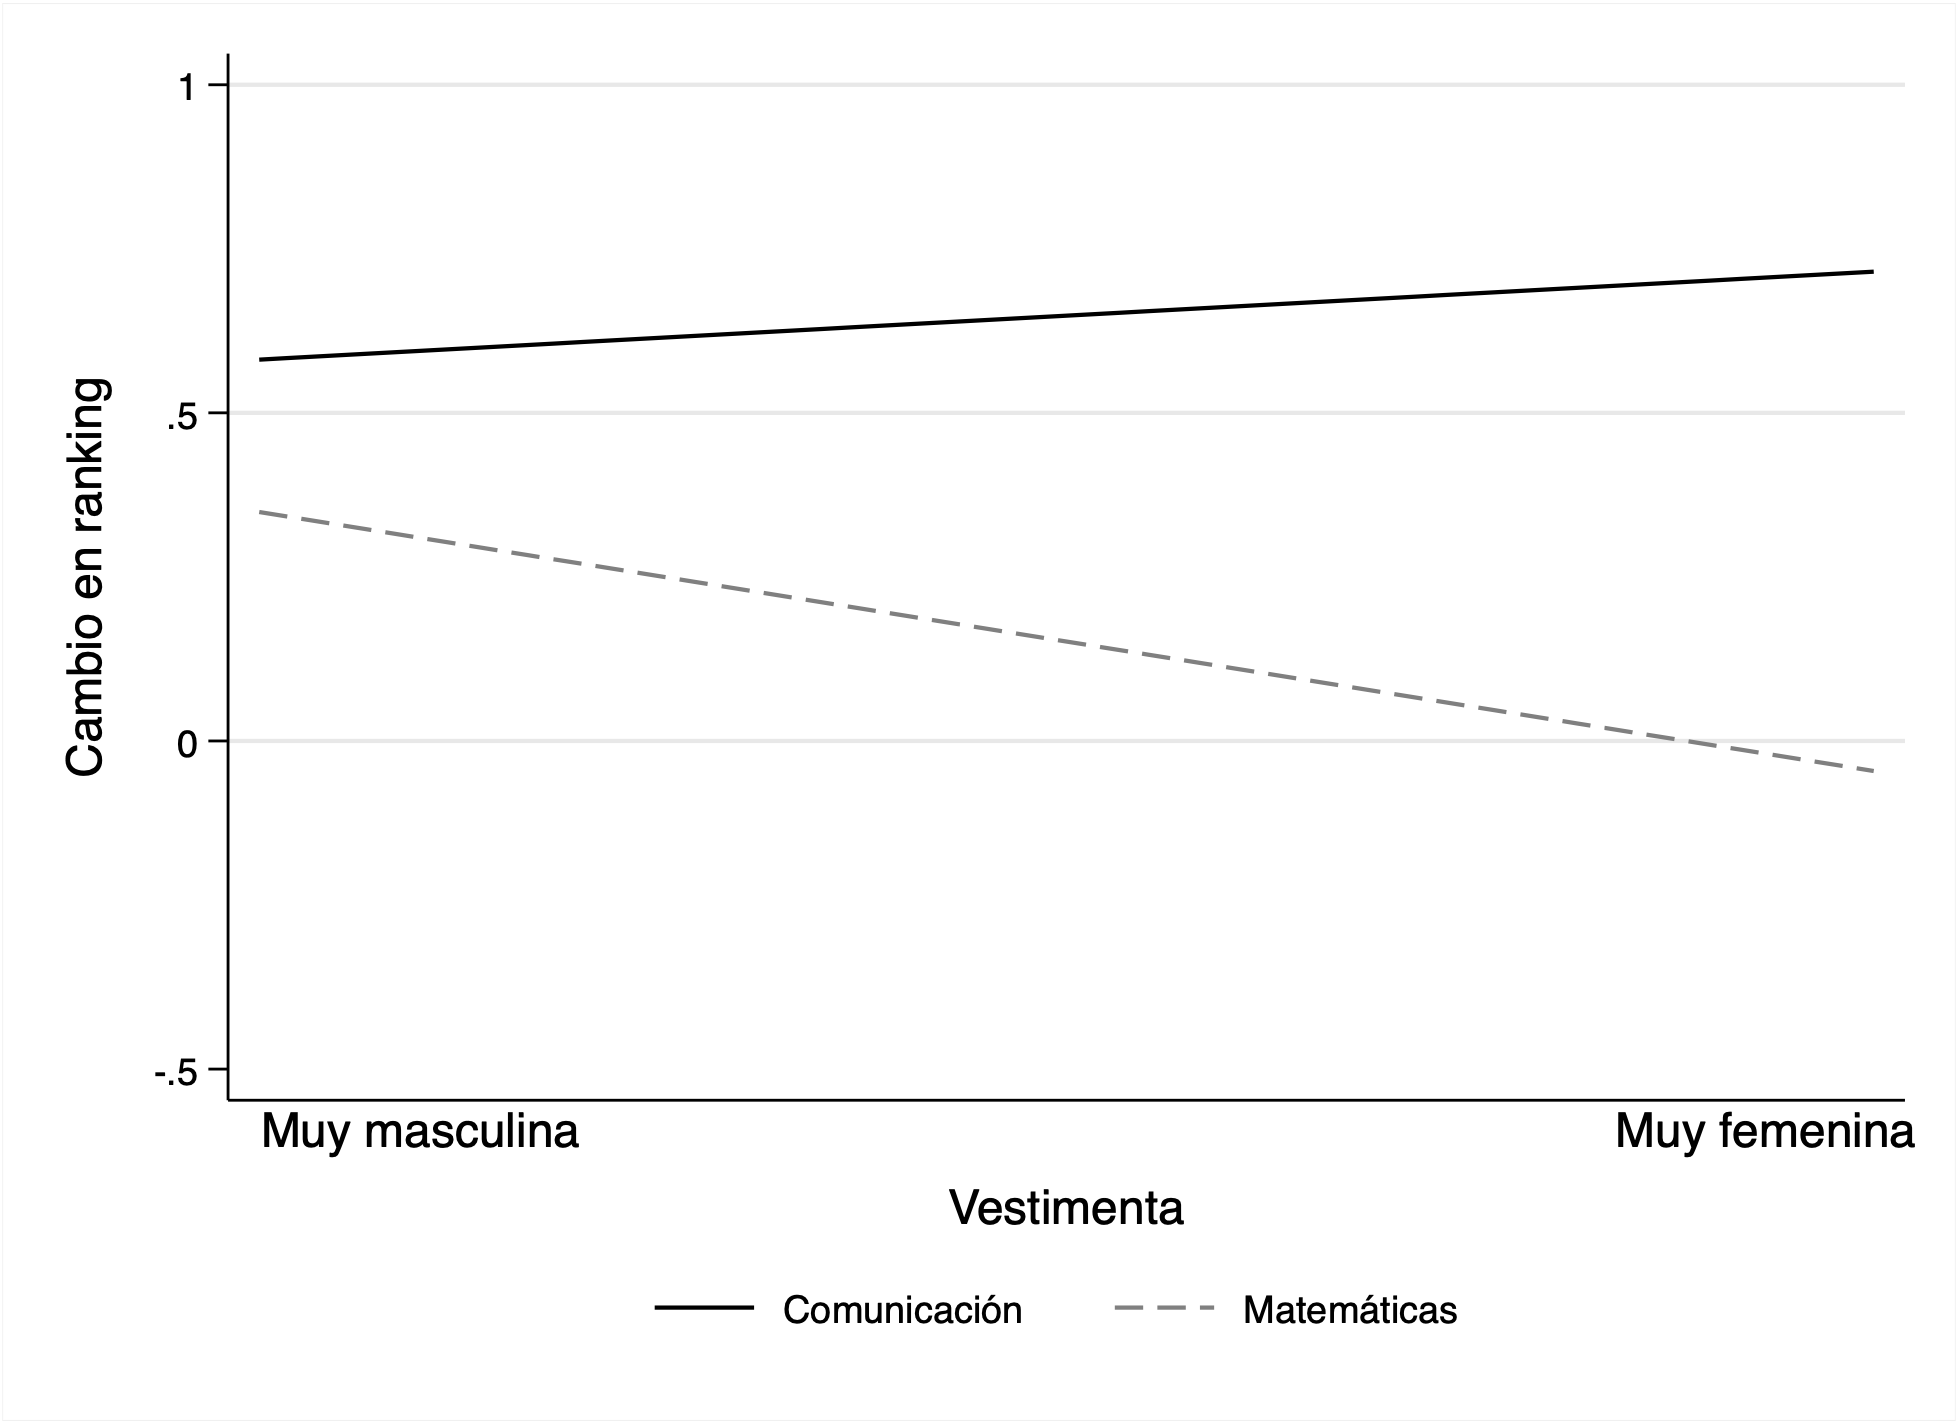
\includegraphics[width=7.8cm]{Images/h1_predicted_rank_score.png}
    \end{subfigure}
    \begin{minipage}{0.245\textwidth}
        
    \end{minipage}
    \centering
    \begin{subfigure}[t]{0.49\textwidth}
        \centering
        \caption{Rankers femeninos}
        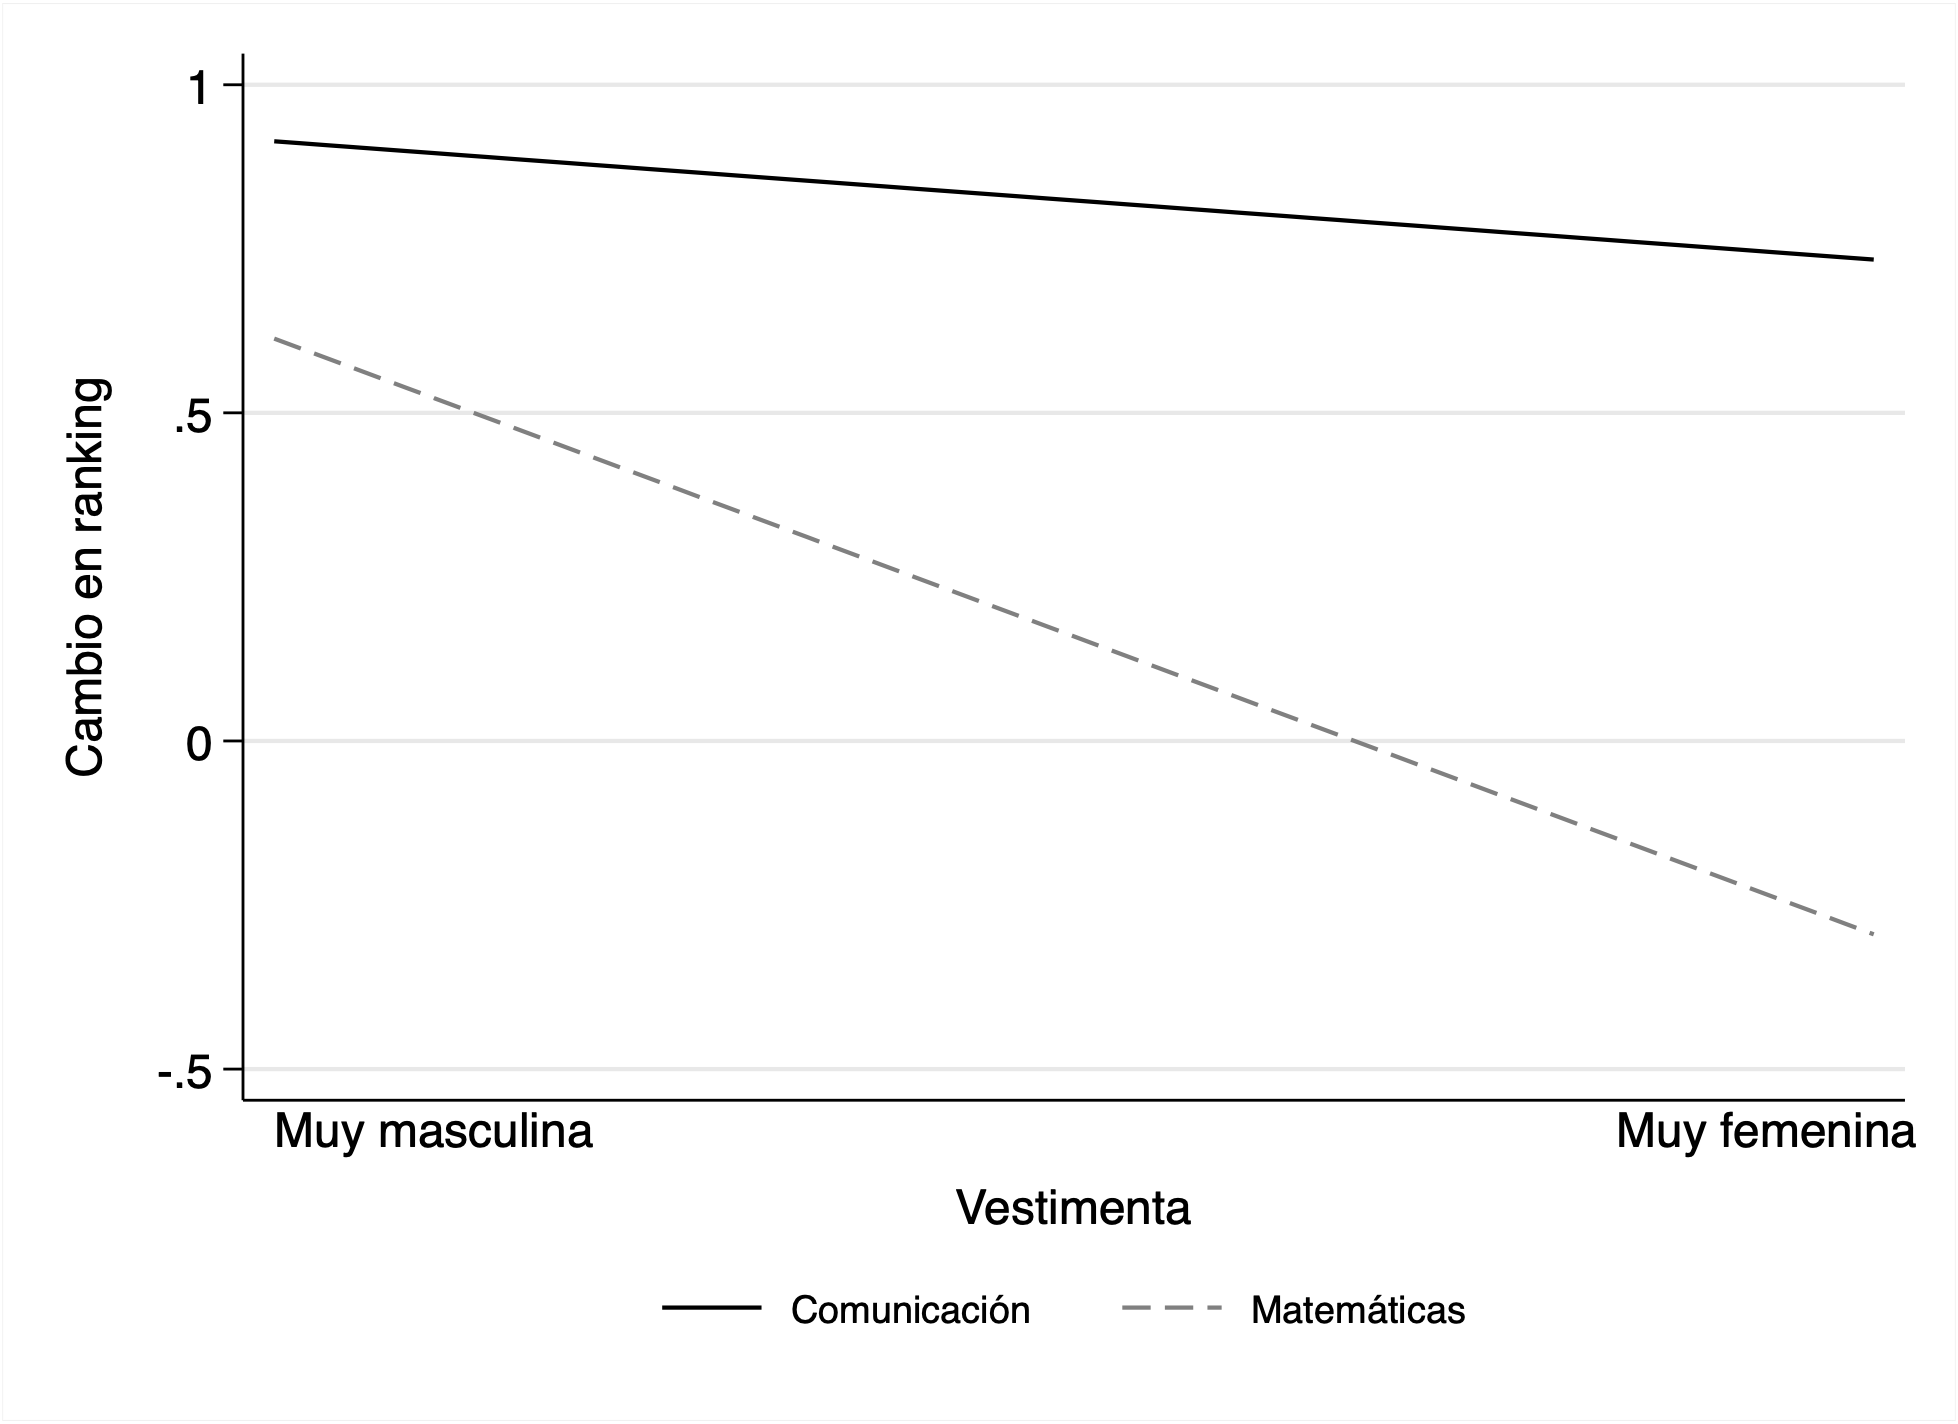
\includegraphics[width=7.8cm]{Images/h2_predicted_rank_score_fem.png}
    \end{subfigure}
    \begin{subfigure}[t]{0.49\textwidth}
        \centering
        \caption{Rankers masculino}
        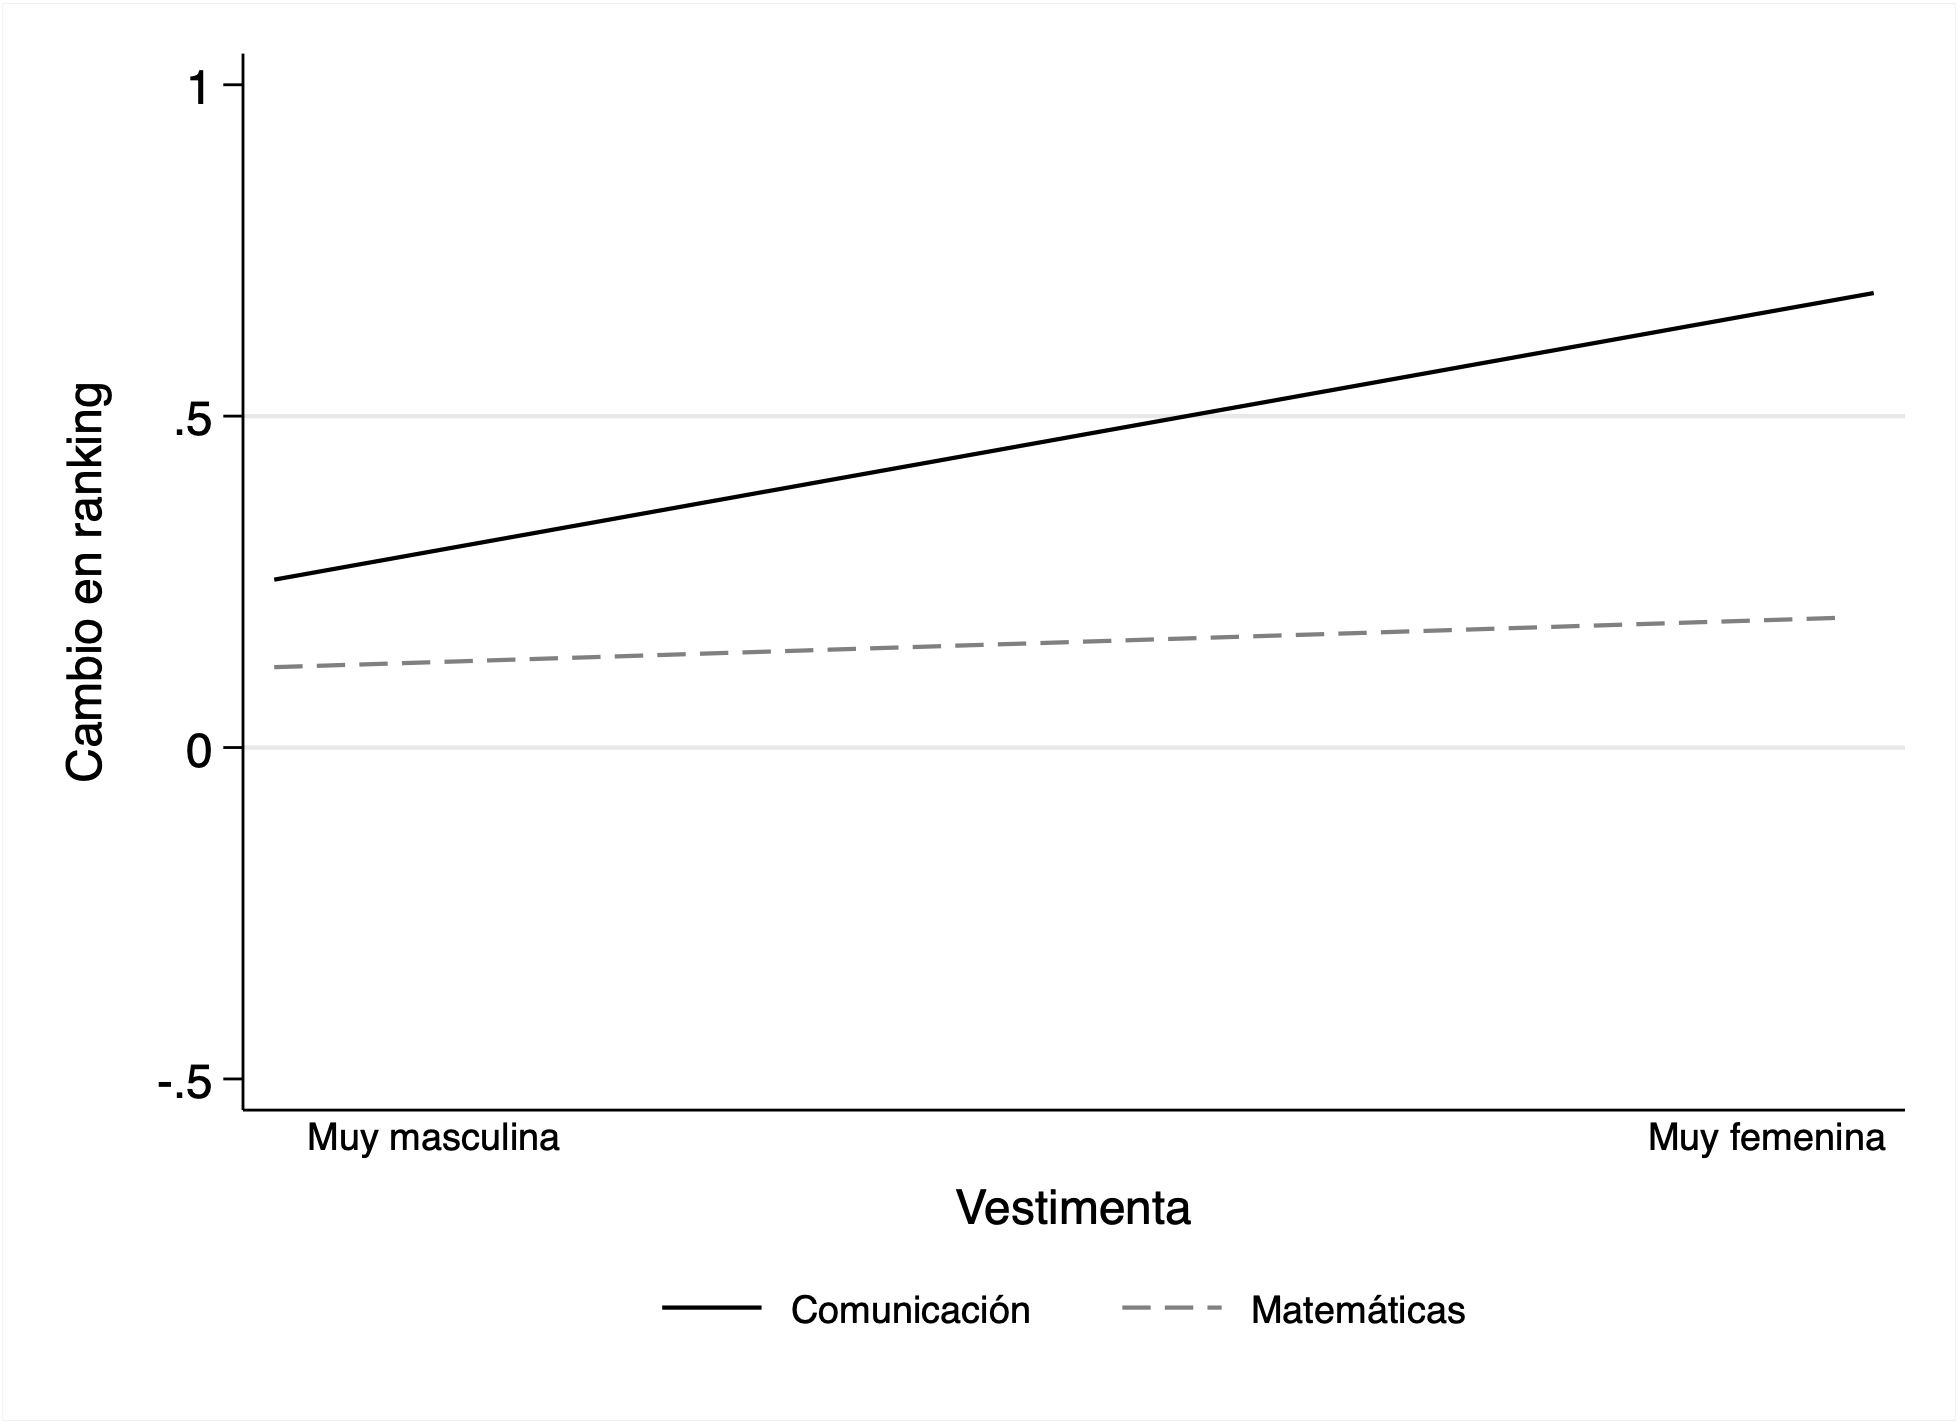
\includegraphics[width=7.8cm]{Images/h2_predicted_rank_score_masc.png}
    \end{subfigure}
    \begin{subfigure}[t]{0.49\textwidth}
        \centering
        \caption{Compliers}
        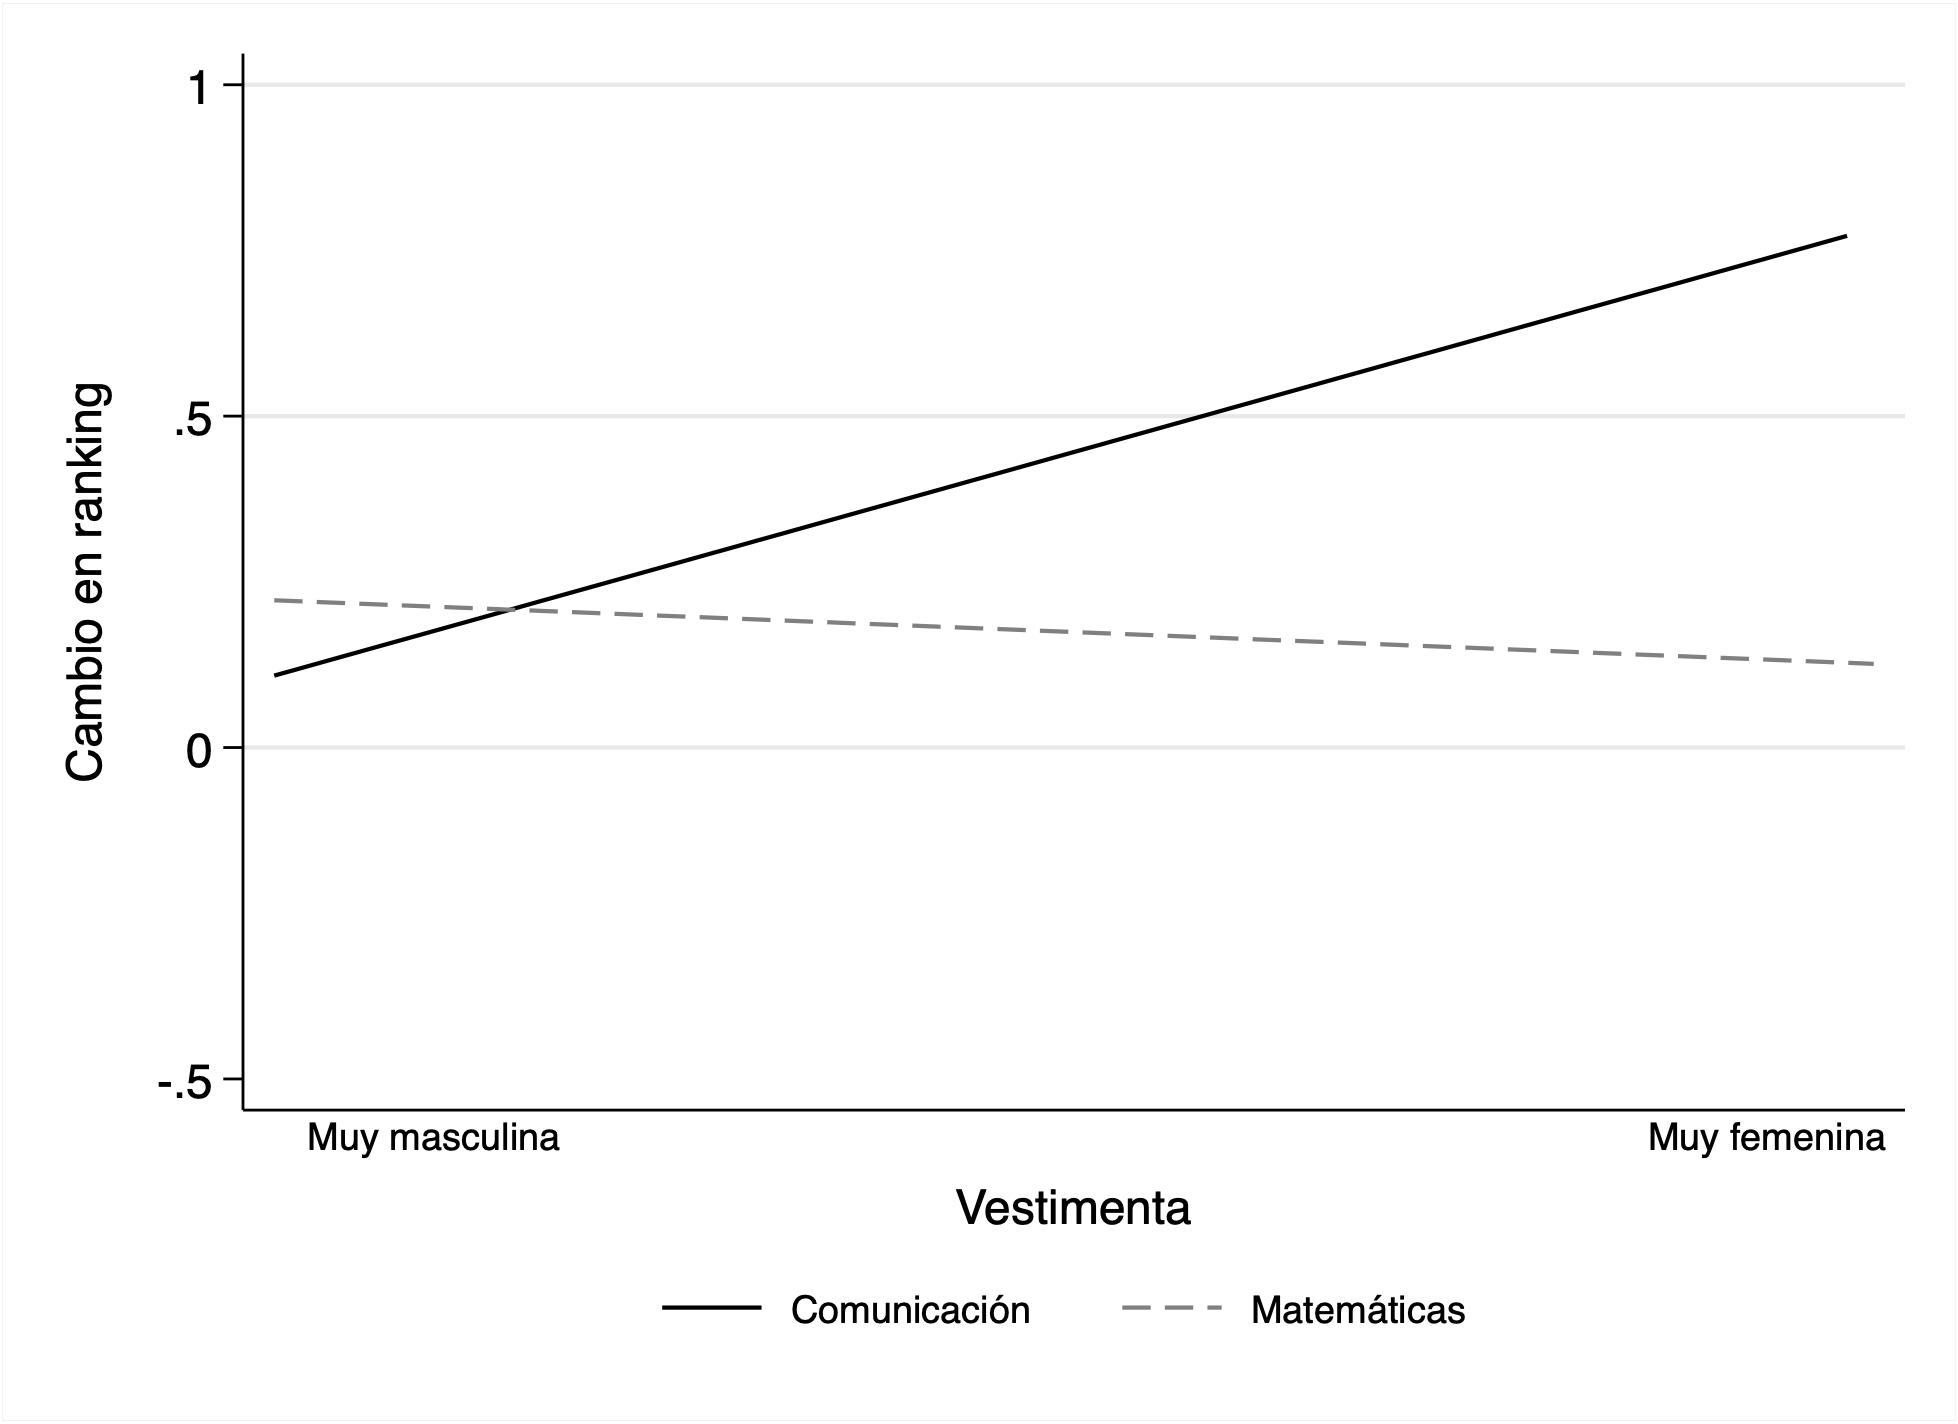
\includegraphics[width=7.8cm]{Images/h3_predicted_rank_score_complier.png}
    \end{subfigure}
    \begin{subfigure}[t]{0.49\textwidth}
        \centering
        \caption{No compliers}
        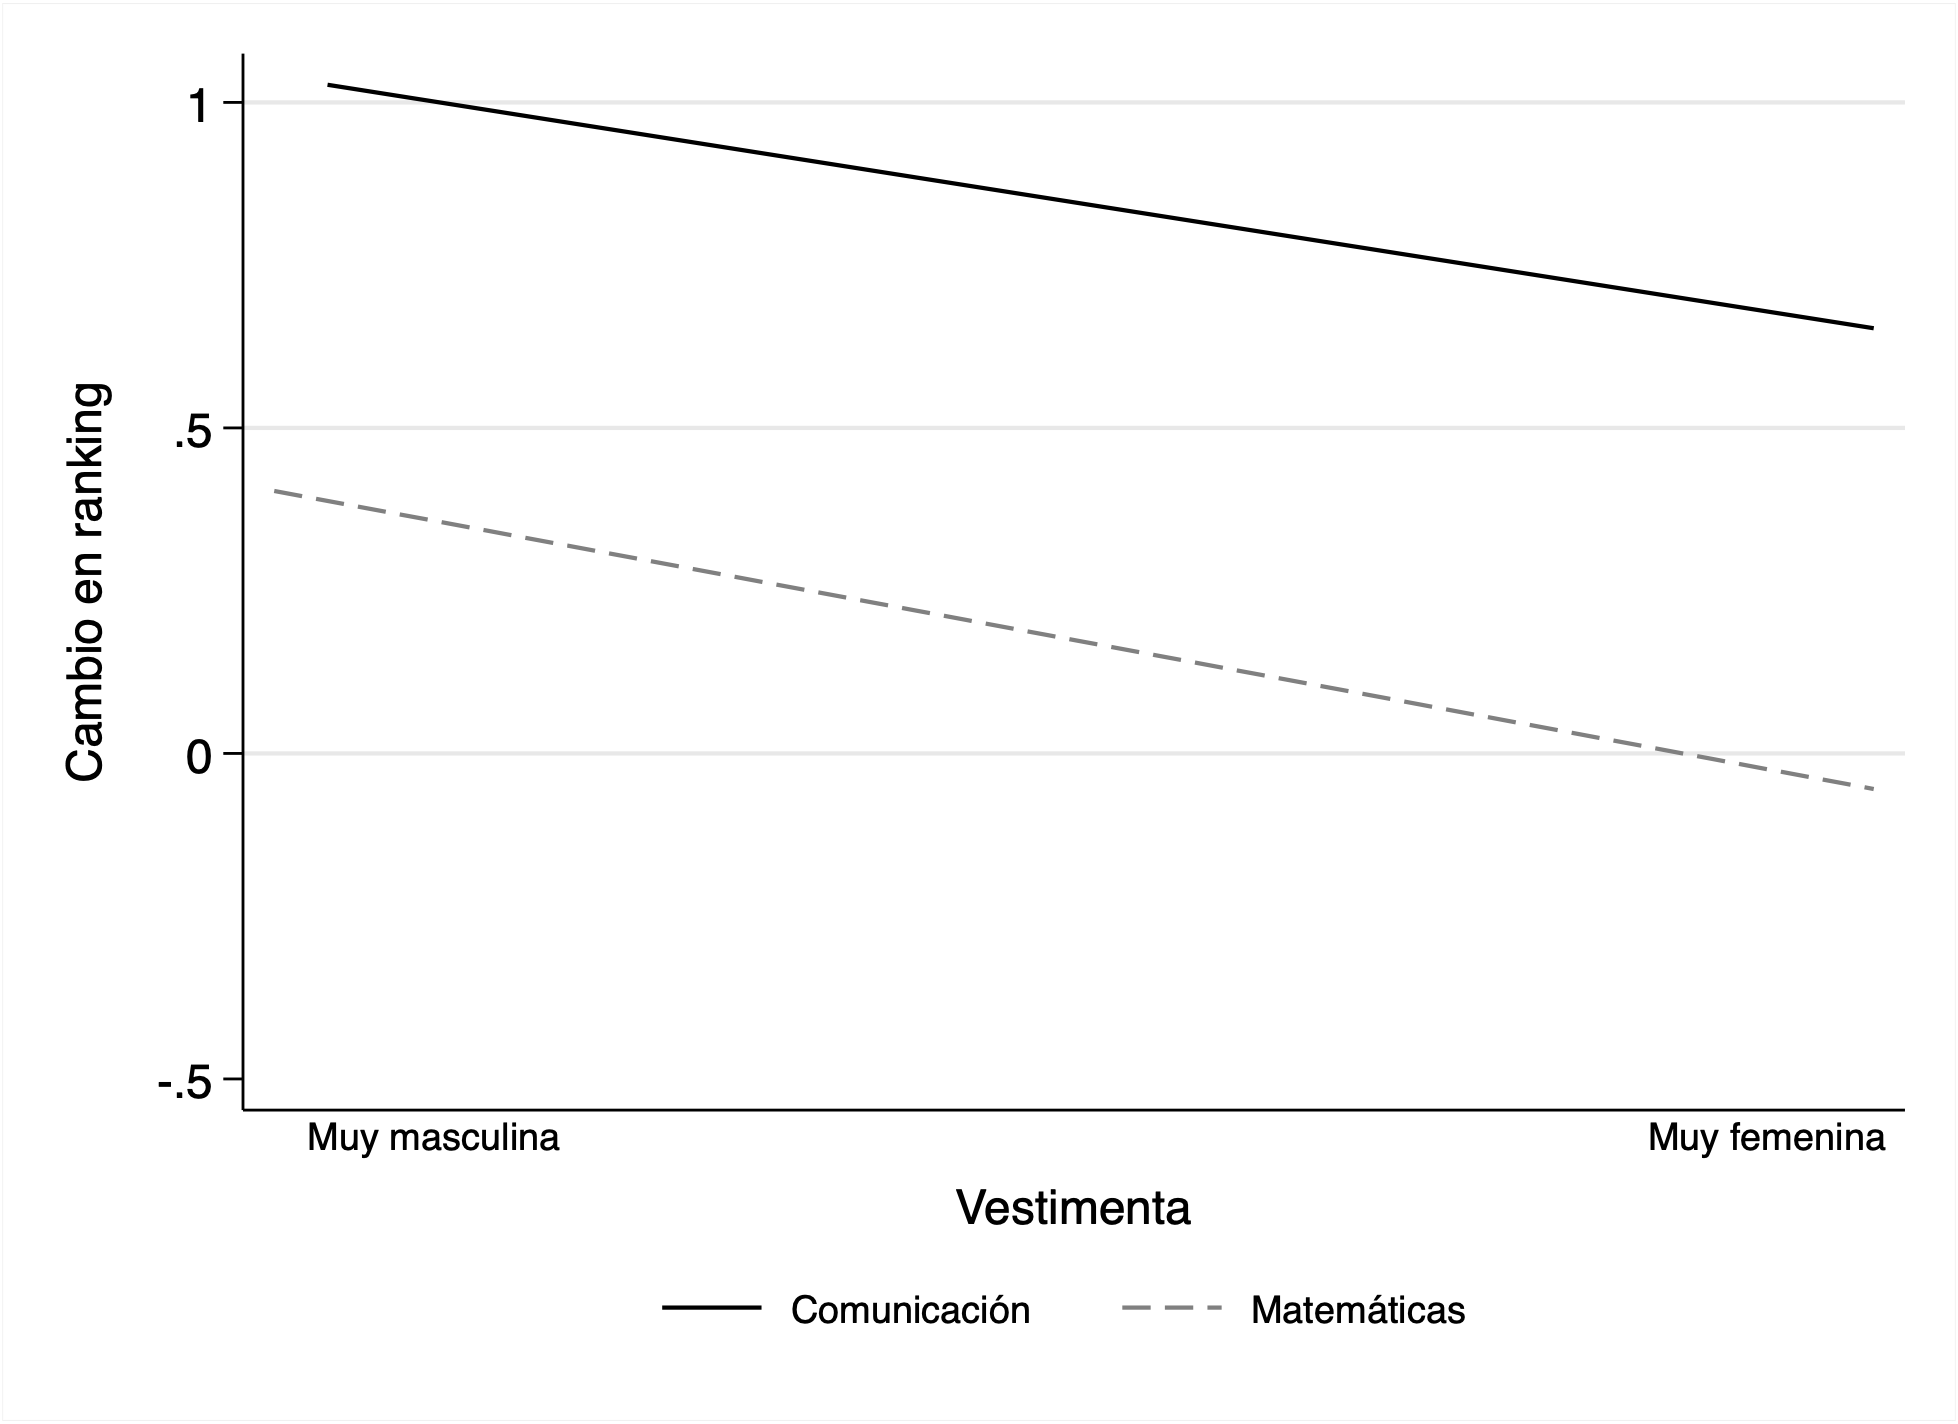
\includegraphics[width=7.8cm]{Images/h3_predicted_rank_score_nocomplier.png}
    \end{subfigure}
\end{figure}
 
Ahora bien, cuando el ranker era de identidad femenina, el efecto de cambiar la vestimenta de muy femenina a muy masculina, condicional a que la habilidad principal eran las matemáticas, es de un aumento de 0.4 d.e. en el \textit{ranking}. Por el contrario, cuando la habilidad principal de sus pares era la comunicación, baja el ranking en 0.08d.e. En resumen, los \textit{rankers} de identidad femenina presentaron una preferencia por trabajar con pares que tenían vestimenta masculina y su habilidad principal era la comunicación, y el tipo de persona con la que estaban menos dispuestos a interactuar era con aquellos que tenían vestimenta muy femenina y su habilidad principal eran las matemáticas. 

Cuando el \textit{ranker} era de identidad masculina, las personas con vestimenta femenina y hábiles comunicándose recibieron el mejor ranking. En esta submuestra, el efecto de pasar de tener una vestimenta muy masculina a tener una muy femenina, cuando la habilidad principal era la comunicación, en está submuestra, es de 0.19d.e. Un efecto tres veces más grande que el de la muestra completa. Por el contrario, cuando la habilidad principal eran las matemáticas, los \textit{rankers} de identidad masculina fueron prácticamente indiferentes de la vestimenta. 

\begin{table}
    \centering
    \caption{Diferencia en \textit{ranking} por combinaciones de expresiones de género y tipo de \textit{ranker}}
    \begin{subtable}{\textwidth}
        \centering
        \caption{Todos}
        \fontsize{9.5}{12}\selectfont {
        \begin{tabular}{cccccc}\hline \hline
                                         &	\multicolumn{2}{c}{\textit{Comunicación}}   &   
                                         &	\multicolumn{2}{c}{\textit{Matemáticas}}	\\ \cmidrule{2-3} \cmidrule{5-6}
                                         &  \textit{Vest. F}    &   \textit{Vest. M}    &   
                                         &  \textit{Vest. F}    &   \textit{Vest. M}    \\ \hline
        \textit{Vest. F \& Comunicación} &	-	                &   0.13                &   
                                         &   0.76               &  	0.37                \\
        \textit{Vest. M \& Matemáticas } &  -0.37	            &   -0.23	            &   
                                         &   0.39               &     -	                \\ \hline\hline
    \end{tabular}}
    \end{subtable}
    \begin{subtable}{\textwidth}
        \centering
        \vspace*{0.5cm}
        \caption{\textit{Ranker} femenino}
        \fontsize{9.5}{12}\selectfont {
        \begin{tabular}{cccccc}\hline \hline
                                         &	\multicolumn{2}{c}{\textit{Comunicación}}   &   
                                         &	\multicolumn{2}{c}{\textit{Matemáticas}}	\\ \cmidrule{2-3} \cmidrule{5-6}
                                         &  \textit{Vest. F}    &   \textit{Vest. M}    &   
                                         &  \textit{Vest. F}    &   \textit{Vest. M}    \\ \hline
        \textit{Vest. F \& Comunicación} &  -	                &   -0.18               &   
                                         &  1.03                &   0.12                \\
        \textit{Vest. M \& Matemáticas } &  -0.12	            &   -0.30	            &   
                                         &  0.91                &   -	                \\ \hline\hline
        \end{tabular}}
    \end{subtable}
    \begin{subtable}{\textwidth}
        \centering
        \vspace*{0.5cm}    
        \caption{Ranker masculino}
        \fontsize{9.5}{12}\selectfont {
        \begin{tabular}{cccccc}\hline \hline
                                         &	\multicolumn{2}{c}{\textit{Comunicación}}   &   
                                         &	\multicolumn{2}{c}{\textit{Matemáticas}}	\\ \cmidrule{2-3} \cmidrule{5-6}
                                         &  \textit{Vest. F}    &   \textit{Vest. M}    &   
                                         &  \textit{Vest. F}    &   \textit{Vest. M}    \\ \hline
        \textit{Vest. F \& Comunicación} &	-	                &   0.43                &   
                                         &  0.49                & 	0.56                \\
        \textit{Vest. M \& Matemáticas}  &  -0.56	            &   -0.13	            &   
                                         &  -0.08               &   -	                \\ \hline\hline
        \end{tabular}}
    \end{subtable}
    \begin{subtable}{\textwidth}
        \centering
        \vspace*{0.5cm} 
        \caption{\textit{Compliers}}
        \fontsize{9.5}{12}\selectfont {
        \begin{tabular}{cccccc}\hline \hline
                                         &	\multicolumn{2}{c}{\textit{Comunicación}}   &   
                                         &	\multicolumn{2}{c}{\textit{Matemáticas}}	\\ \cmidrule{2-3} \cmidrule{5-6}
                                         &  \textit{Vest. F}    &   \textit{Vest. M}    &   
                                         &  \textit{Vest. F}    &   \textit{Vest. M}    \\ \hline
        \textit{Vest. F \& Comunicación} &	-	                &   0.67                &   
                                         &  0.66                & 	0.56                \\
        \textit{Vest. M \& Matemáticas } &  -0.56	            &   0.11	            &   
                                         &  0.10                &    -	                \\ \hline\hline
        \end{tabular}}
    \end{subtable}
    \begin{subtable}{\textwidth}
        \centering
        \vspace*{0.5cm}
        \caption{No \textit{Compliers}}
        \fontsize{9.5}{12}\selectfont {
        \begin{tabular}{cccccc}\hline \hline
                                         &	\multicolumn{2}{c}{\textit{Comunicación}}   &   
                                         &	\multicolumn{2}{c}{\textit{Matemáticas}}	\\ \cmidrule{2-3} \cmidrule{5-6}
                                         &  \textit{Vest. F}    &   \textit{Vest. M}    &   
                                         &  \textit{Vest. F}    &   \textit{Vest. M}    \\ \hline
        \textit{Vest. F \& Comunicación} &	-	                &   -0.39               &   
                                         &  0.70                & 	0.25                \\
        \textit{Vest. M \& Matemáticas } &  -0.25	            &   -0.64	            &   
                                         &  0.46                &   -	                \\ \hline\hline
        \end{tabular}}
    \end{subtable}
    \begin{threeparttable}
    \begin{tablenotes}
    \scriptsize{
    \item Nota: Vest. F corresponde a una vestimenta muy femenina (1.5d.e arriba del promedio) y Vest. M corresponde a una vestimenta muy masculina (1.5d.e abajo del promedio). El valor corresponde a la fila menos la columna. Si el valor es positivo, es porque la combinación de expresiones de género de la fila tiene un mejor ranking que la combinación de la columna. Por ejemplo, una persona con todas vestimenta y habilidad femeninas en promedio está 0.13 puestos más arriba en el ranking que una que tiene una vestimenta femenina y habilidad masculina (Panel (a), la fila superior, segunda columna).}
    \end{tablenotes}
    \end{threeparttable}
    \label{tab:hypothesis_tables}
\end{table}

\begin{result}
Existen diferencias en la disposición a interactuar de \textit{rankers} femeninos y masculinos ante diferentes combinaciones de expresiones de género. 
\end{result}

\begin{table}
    \centering
    \caption{Diferencia en ranking entre género del ranker por combinaciones de expresiones de género}
    \label{tab:Diffs}
    \begin{subtable}{0.49\textwidth}
    \centering
    \caption{Por género del \textit{ranker}}
    \fontsize{9.5}{12}\selectfont {
    \begin{tabular}{ccccc}\hline \hline
          \multicolumn{2}{c}{\textit{Comunicación}} &   
        & \multicolumn{2}{c}{\textit{Matemáticas}}	\\ \cmidrule{1-2} \cmidrule{4-5}
          \textit{Vest. F}  &   \textit{Vest. M}    &   
        & \textit{Vest. F}  &   \textit{Vest. M}    \\ \hline
	      0.05	            &   0.66                &
	    & -0.49             &   0.49                \\ \hline \hline
    \end{tabular}}
    \end{subtable}
    \begin{subtable}{0.49\textwidth}
    \centering
    \caption{Por \textit{compliance} del \textit{ranker}}
    \fontsize{9.5}{12}\selectfont {
    \begin{tabular}{ccccc}\hline \hline
          \multicolumn{2}{c}{\textit{Comunicación}} &   
        & \multicolumn{2}{c}{\textit{Matemáticas}}  \\ \cmidrule{1-2} \cmidrule{4-5}
          \textit{Vest. F}  &   \textit{Vest. M}    &   
        & \textit{Vest. F}  &   \textit{Vest. M}    \\ \hline
	      0.13	            &   -0.93               &
	    & 0.18              &   -0.18               \\ \hline \hline
    \end{tabular}}
    \end{subtable}
    \begin{threeparttable} 
    \begin{tablenotes}
    \scriptsize{
    \item Nota: Vest. F corresponde a una vestimenta muy femenina (1.5d.e arriba del promedio) y Vest. M corresponde a una vestimenta muy masculina (1.5d.e abajo del promedio). En el panel (a) el valor corresponde a la diferencia entre la posición promedio que en la que una persona de identidad femenina a un perfil con esa combinación de expresiones de género y la posición promedio que una persona de identidad masculina le da a ese mismo perfil. En el panel (b) el valor corresponde a la diferencia entre la posición promedio que en la que una persona que es \textit{complier} a un perfil con esa combinación de expresiones de género y la posición promedio que una persona que no es \textit{complier} le da a ese mismo perfil.}
    \end{tablenotes}
    \end{threeparttable}
\end{table}

Por último, hay una diferencia en la manera en la que responden a las combinaciones de expresiones de género los participantes que se adhieren a la norma social con sus expresiones de género y los que no se adhieren. Los participantes que son \textit{compliers} con sus expresiones de género, presentaron una preferencia por trabajar con los pares que eran hábiles comunicándose y que tenían una vestimenta femenina. En el orden de los \textit{compliers}, cuando la habilidad principal era la comunicación, pasar de tener una vestimenta muy masculina a una muy femenina, aumentaba el \textit{ranking} en 0.29d.e. Mientras que, cuando la habilidad principal eran las matemáticas, la diferencia entre el ranking que le daban los \textit{compliers} a sus pares era prácticamente independiente a la vestimenta que tuvieran.

Por la otra parte, cuando la persona que organizaba los perfiles no se adhería a la norma social con sus expresiones de género, estos mostraron una preferencia por trabajar con las personas que presentaban una vestimenta masculina y cuya habilidad principal era la comunicación. Lo que resulta interesante de las elecciones de los \textit{rankers} que no fueron \textit{compliers} es que pareciera que no tuvieron en cuenta la habilidad y la vestimenta conjuntamente. Estos \textit{rankers} prefirieron personas hábiles comunicándose siempre en la misma magnitud que las personas hábiles en matemáticas, independiente de su vestimenta. De igual modo, presentaron una preferencia frente a las personas con vestimenta masculina por encima de las que tenían vestimenta femenina, independiente a la habilidad. 
\begin{result}
Existen diferencias en la disposición a interactuar de \textit{rankers} que se adhieren la norma social con sus expresiones de género y los que no se adhieren, ante diferentes combinaciones de expresiones de género. 
\end{result}
\section{Discusión}
Este trabajo encuentra que en promedio los agentes tienen expresiones de género acordes a lo socialmente prescrito para su identidad. También encuentra que, en promedio, hay una baja disposición a trabajar en grupo con personas que tenían una vestimenta femenina y reportaban que su habilidad principal eran las matemáticas. Esa baja disposición a trabajar con personas con esas características, puede estar fundamentado en la creencia de que su aporte al desarrollo del meme pudiera ser menor al aporte de personas con otras características. Sin embargo, las personas con vestimenta femenina, hábiles en matemáticas, fueron las que obtuvieron el mejor desempeño (ver figura \ref{fig:performance}). 

\begin{figure}[htbp]
    \centering
    \begin{subfigure}{0.49\textwidth}
        \centering
        \caption{Ranking promedio}
        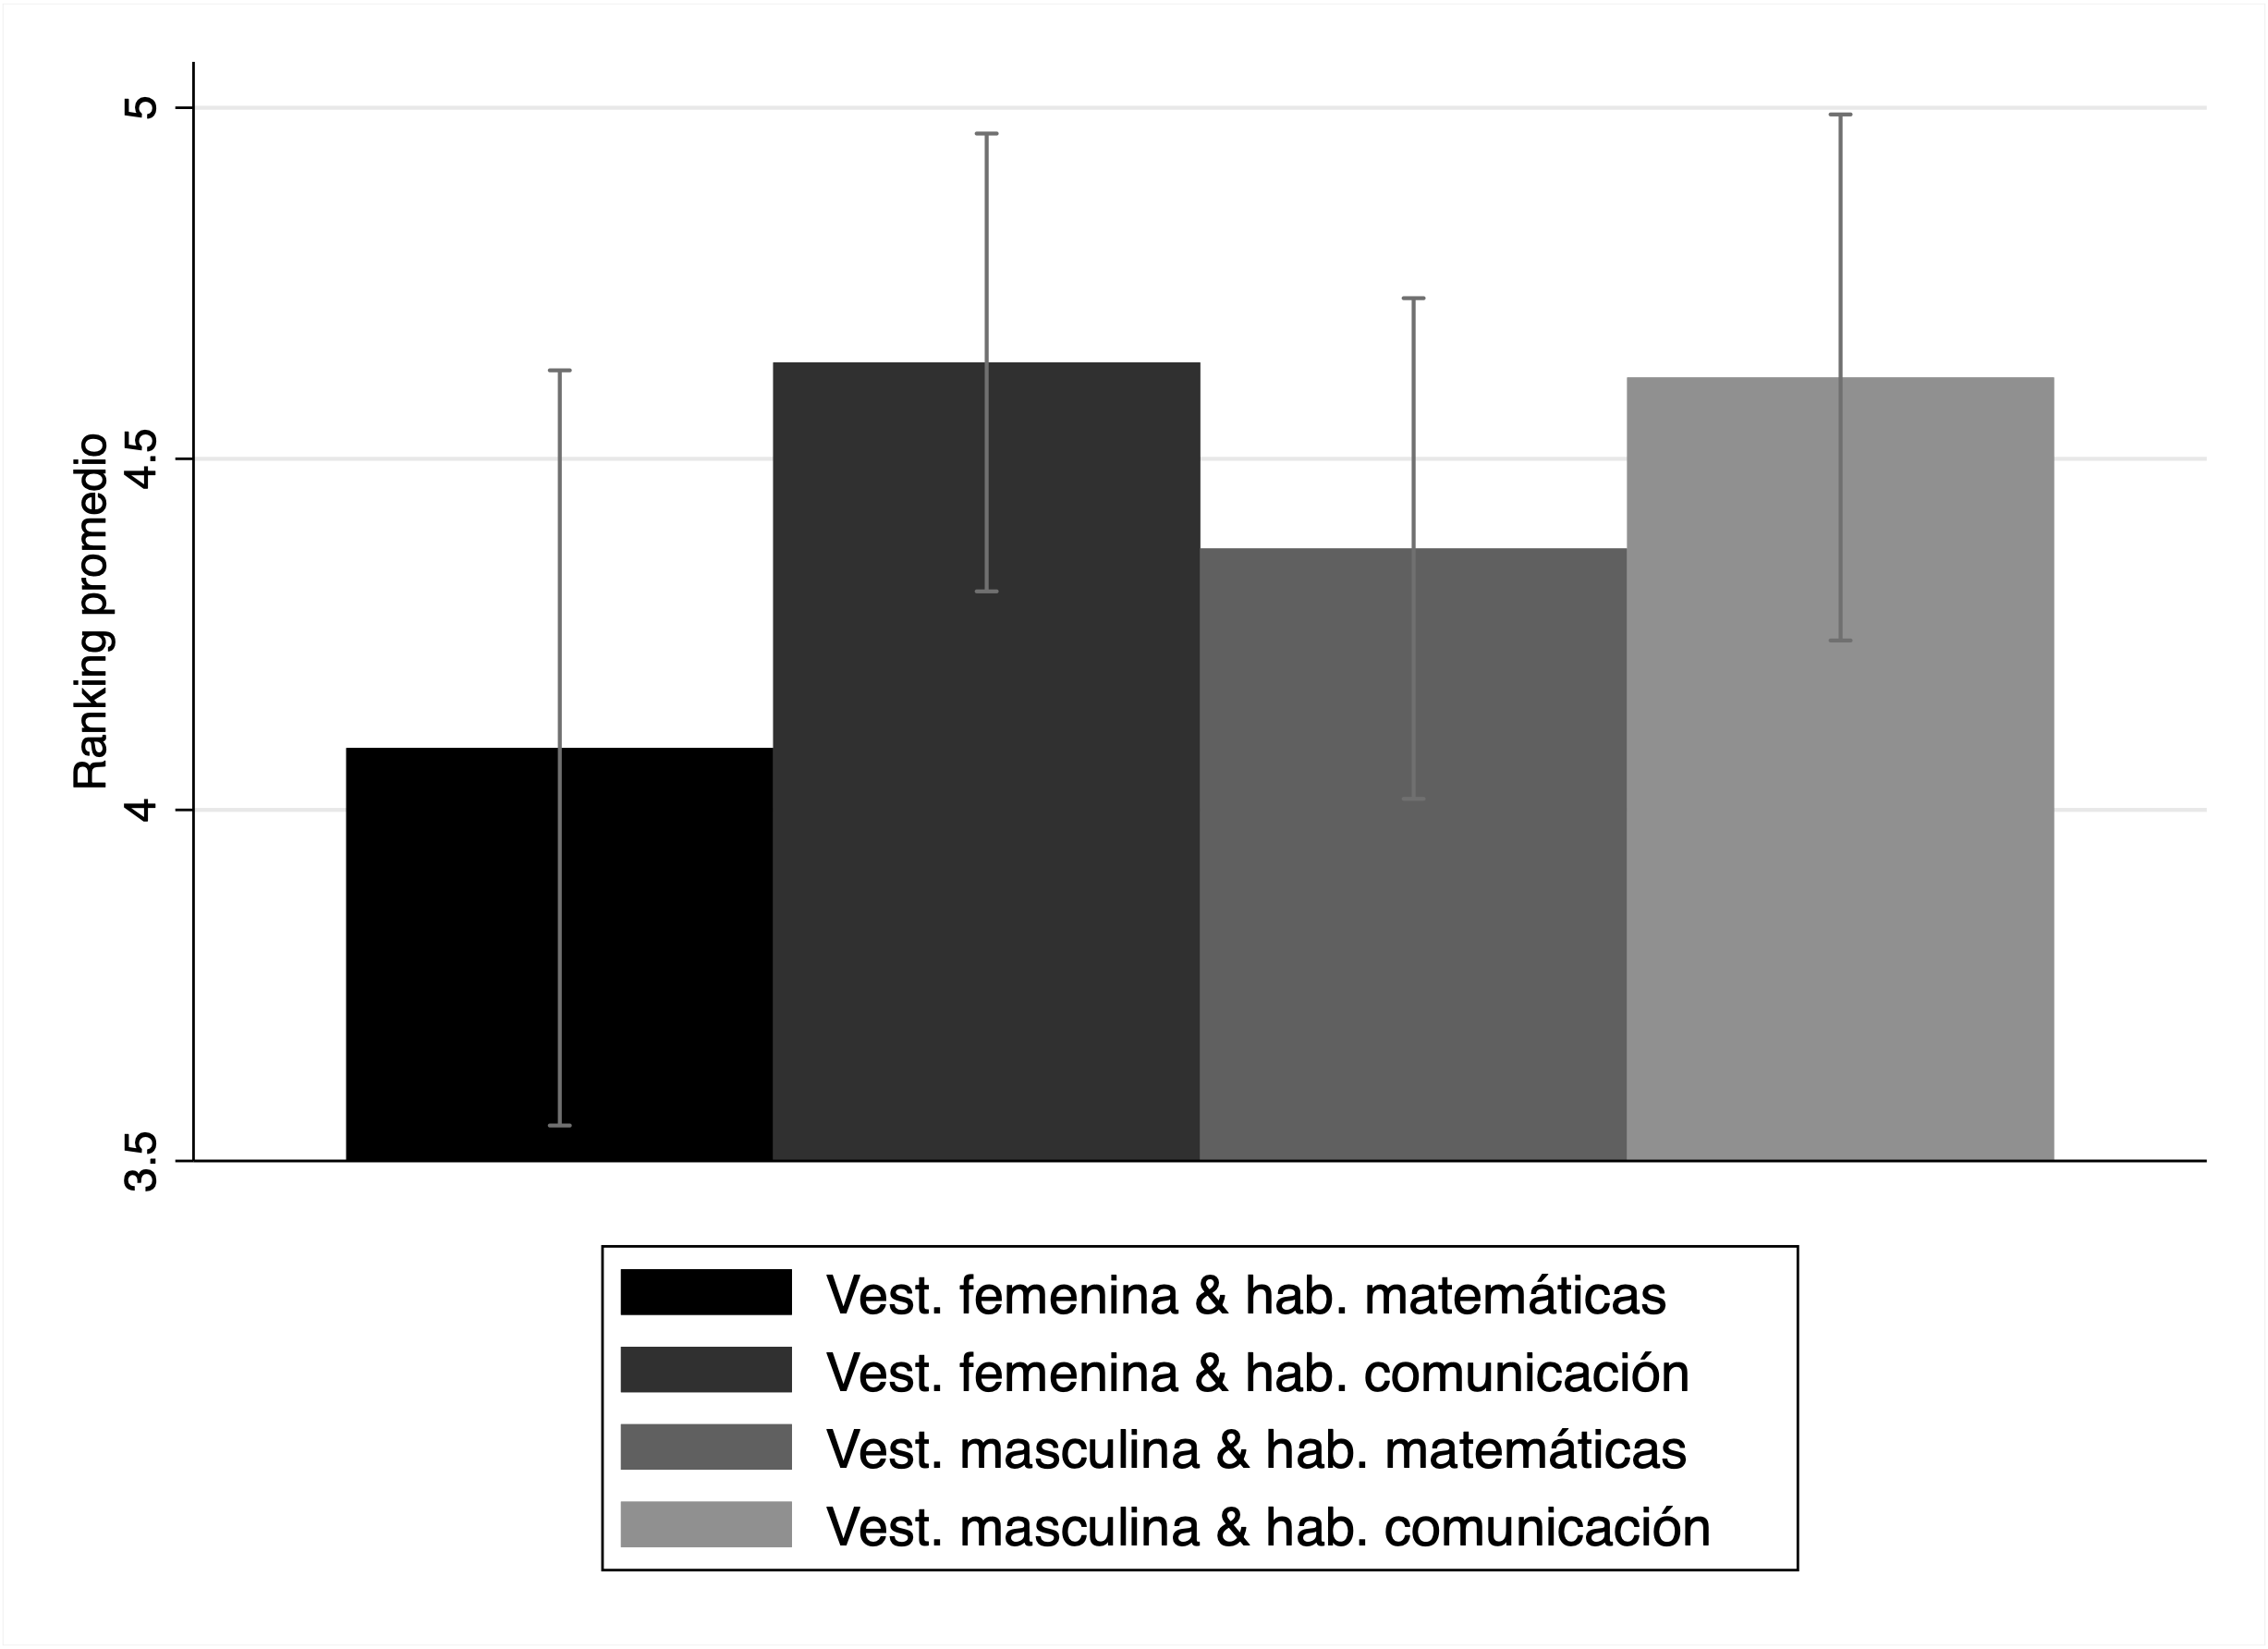
\includegraphics[width=\textwidth]{Images/ranking.png}
    \end{subfigure}
    \begin{subfigure}{0.49\textwidth}
        \centering
        \caption{Desempeño promedio}
        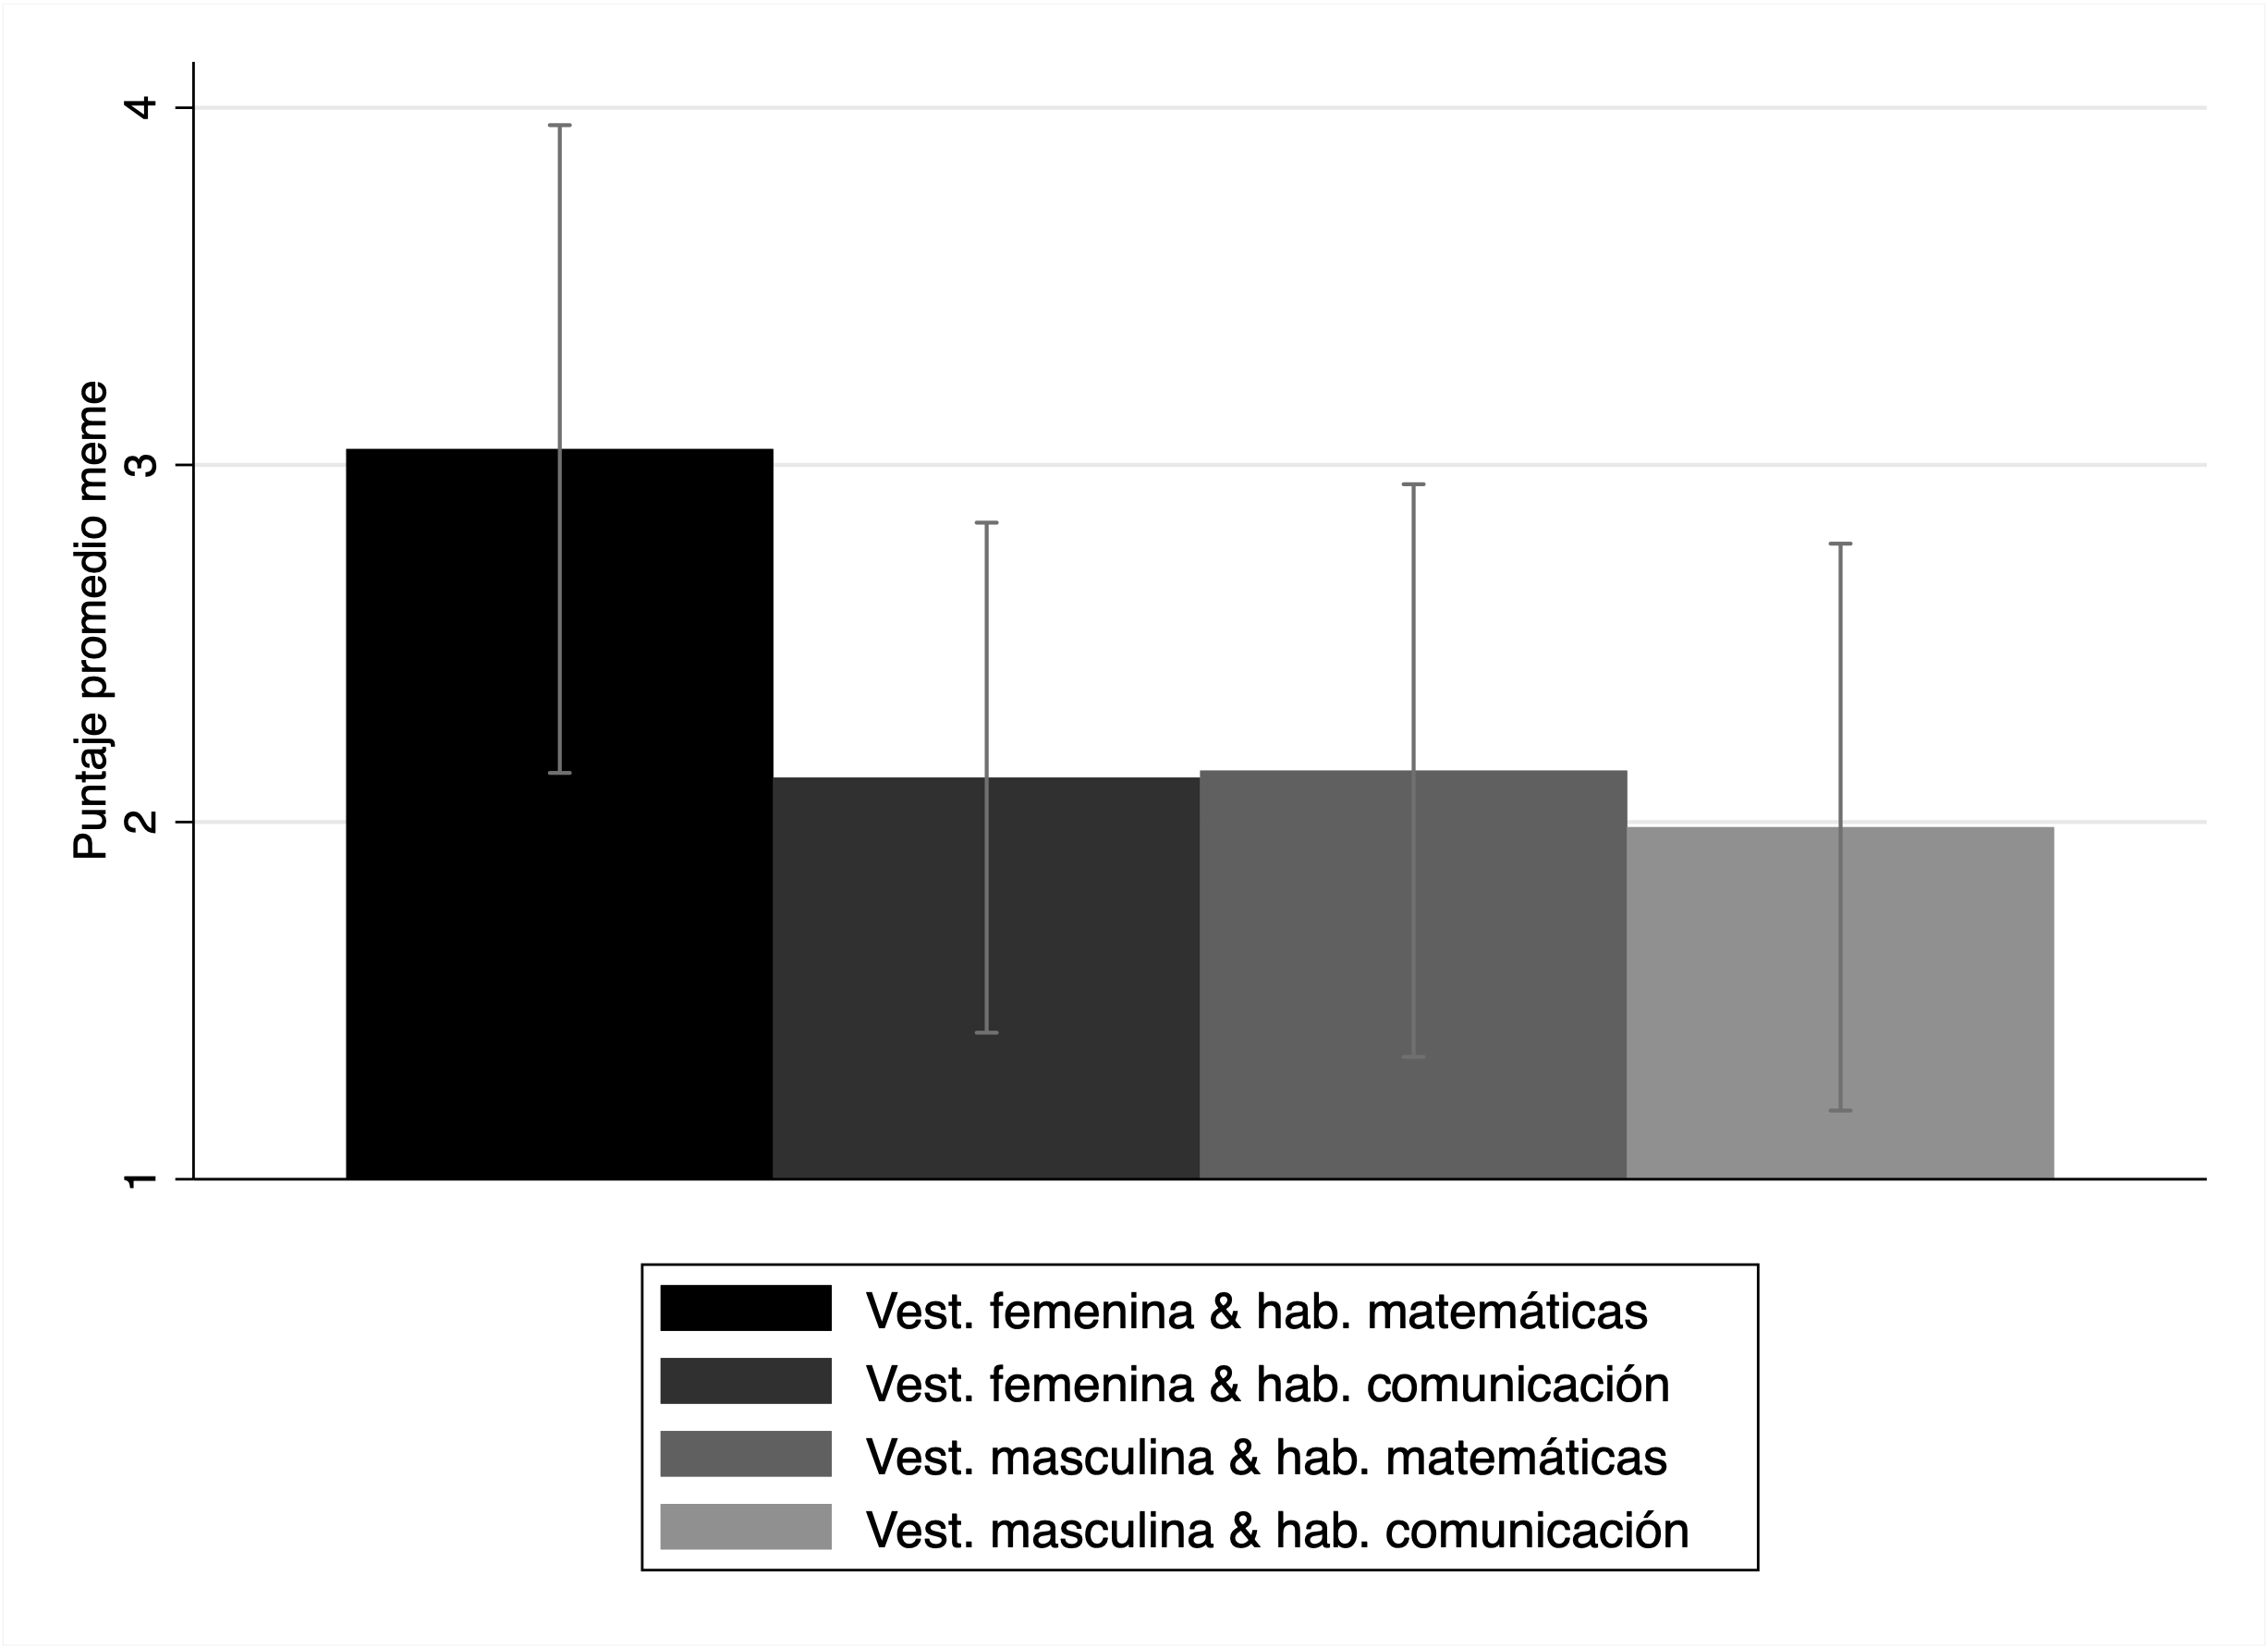
\includegraphics[width=\textwidth]{Images/performance.png}
    \end{subfigure}
    \caption{Ranking y desempeño promedio por conjunto de expresiones de género}
    \label{fig:performance}
    \begin{singlespace}
    \floatfoot{\footnotesize{\textit{Nota:} Gráficas del \textit{ranking} y desempeño promedio. El desempeño promedio corresponde al promedio del puntaje que cada juez le dio al \textit{meme} Intervalos de confianza al 95\%. }\par}
    \end{singlespace}
\end{figure}

El desempeño, definido como el promedio del puntaje (de 0 a 5) que cada juez le dio al \textit{meme}, ignora el aporte de cada persona del grupo al \textit{meme}. Pero, si en efecto existe algún grado de relación entre las características y el desempeño, si la población de participantes se hubiera segmentado entre personas con vestimenta femenina, hábiles en matemáticas y el resto de la población, estos últimos habrían tenido un desempeño subóptimo (inferior al desempeño posible). 

\section{Conclusiones}
Este trabajo estudia de qué manera, observar diferentes expresiones de género, cuando la identidad de género es información privada, cambia la disposición a interactuar entre pares. Para esto, este trabajo primero presenta un juego de información incompleta en el que la identidad de uno de los jugadores es información privada. Ese jugador conoce su identidad y debe elegir entre tener un expresión de género femenina o una masculina. El otro jugador observa la expresión de género de ese agente, a partir de esto forma creencias sobre la identidad del dicho agente y decide si interactúa o no con él. Segundo, este trabajo incluye un experimento de campo en el que los participantes debían elegir con quién desarrollar una tarea, únicamente con la información de unas de sus expresiones de género, la edad y el departamento de nacimiento. 

Los resultados del modelo sugieren que existen dos condiciones principales para que los agentes lleguen a un equilibrio en el que interactúen y en el que el jugador, con información privada, tome una acciones diferente dependiendo de su identidad (tal como sucede en los datos). Primero, si el jugador con información privada es de identidad femenina o de identidad masculina, debe adherirse a la norma social. Es decir, debe tener una expresión femenina o masculina, respectivamente. Segundo, el costo de no interactuar debe ser mayor o igual al costo esperado de que el otro jugador esté violando la norma social. 

Los resultados experimentales sugieren que la disposición a interactuar entre pares sí cambia cuando cambia la combinación de expresiones de género que estos observan de los demás. Principalmente hay una baja disposición a interactuar con pares que presentan una vestimenta muy femenina y que reportan ser más hábiles en matemáticas que comunicándose. Dicha baja disposición a interactuar con personas que presenta una vestimenta femenina y que son más hábiles en matemáticas está explicado por la elección de los participantes de identidad femenina. Los resultados también sugieren que entre las vestimentas más masculinas la disposición de sus pares a interactuar con ellos no está determinada por la habilidad. Mientras que entre las vestimentas más femeninas sí hay un beneficio de reportar una habilidad femenina comparado a reportar una habilidad masculina. 

El hecho de que el cumplimiento de las normas sociales cambie la disposición que tienen los demás a interactuar, tiene varias implicaciones. Una de ellas es que genera ineficiencias. Bajo el supuesto de que hay ganancias de interactuar con otros, dejar de hacerlo porque una persona no cumpla una norma social o por un prejuicio implica perder esas ganancias. Por lo tanto, las normas sociales implican un dilema social tanto porque genera que los agentes tengan comportamiento homogéneos aunque no sea consistente con sus preferencias, como porque trunca el desarrollo de redes sociales, que son un mecanismo para mitigar diversos riesgos, el desarrollo de instituciones y el desarrollo económico de una sociedad. 

En efecto, los resultados del experimento sugieren que las personas con la que sus pares estaban menos dispuestas a interactuar, fueron las que obtuvieron el mejor desempeño. Si es en el experimento, en vez de asignar a todas las personas a un grupo, se hubieran sacado a las que obtuvieron el peor ranking, se hubiesen perdido los mejores productos.

Una limitación importante de este trabajo es que no mide si los participantes asocian la vestimenta, las habilidades y las aspiraciones al género. Futuros estudios podrían medirse esta asociación con una prueba de asociación implícita. A pesar de que este trabajo tiene esa limitación, la distribución de expresiones de género por identidades y la encuesta de percepción que se hizo, sugieren que entre los participantes del experimento sí existe la asociación para la vestimenta y la habilidad. 

Otra limitación de este trabajo es que en el experimento, los participantes podían interactuar por correo o celular sin necesidad de encontrarse físicamente. Esto genera que los resultados sean una cuota inferior de la disposición a interactuar. En la encuesta de salida solo el 17\% reporta haberse reunido con su grupo para hacer la tarea. Estudios futuros podrían cambiar el marco del concurso para aumenta la probabilidad de que los participantes interactúen frente a frente. 

Este trabajo también tiene la limitación de que los resultados son sugestivos. Debido a que el tamaño de la muestra es pequeño y por lo que no tiene poder para identificar efectos estadísticamente significativos. Además, el experimento tiene la limitación de que hubo una atrición del 38\% entre la inscripción y el proceso de elección. Esto podría corregirse en futuros estudios recogiendo más información de contacto en la inscripción y acortando los tiempo de las diferentes etapas. 

\vfill
\pagebreak
\begin{appendix}
    \counterwithin{figure}{section}
    \counterwithin{table}{section}
    \section{Equilibrios modelo}

\begin{framed}
\noindent Sean $\gamma_j$ la estrategia del jugador $j$, $k \in \{f,m\}$,  $\theta^e$ el costo esperado por el jugador 2 de que el jugador 1 esté violando la norma social, y $\hat{\theta}^e$ el costo esperado por el jugador 2 fuera de la senda de equilibrio de que el jugador 1 esté violando la norma social,

\noindent (i) $(\gamma_1(k)=\gamma_1(-k)=\gamma_1(o)=E_k, \gamma_2(E_k)=i, \gamma_2(E_{-k})=i)$ es equilibrio si $\eta\in[\theta^e, \infty) \wedge \eta\in[\hat{\theta}^e, \infty) \wedge \Pi_1(E_{k})- \xi \geq \Pi_1(E_{-k})$

\noindent (ii) $(\gamma_1(k)=\gamma_1(-k)=\gamma_1(o)=E_k, \gamma_2(E_k)=i, \gamma_2(E_{-k})=ni)$ es equilibrio si $\eta\in[\theta^e, \infty) \wedge \eta\in (0, \hat{\theta}^e) \wedge \Pi_1(E_{k})- \xi \geq \Pi_1(E_{-k}-\beta)$

\noindent (iii) $(\gamma_1(k)=\gamma_1(-k)=\gamma_1(o)=E_k, \gamma_2(E_k)=ni, \gamma_2(E_{-k})=i)$ es equilibrio si $\eta\in (0, \theta^e) \wedge \eta\in[\hat{\theta}^e, \infty) \wedge \Pi_1(E_{k})- \xi -\beta \geq \Pi_1(E_{-k})$

\noindent (iv) $(\gamma_1(k)=\gamma_1(-k)=\gamma_1(o)=E_k, \gamma_2(E_k)=ni, \gamma_2(E_{-k})=ni)$ es equilibrio si $\eta\in (0, \theta^e) \wedge \eta\in(0, \hat{\theta}^e) \wedge \Pi_1(E_{k})- \xi \geq \Pi_1(E_{-k})$
\end{framed}

\begin{figure}
\caption{Equilibrios agrupadores}
\hspace*{-2cm}
\begin{minipage}{0.49\textwidth}
    \centering
    Si $\theta^e > \hat{\theta}^e$
    
    \scriptsize{
    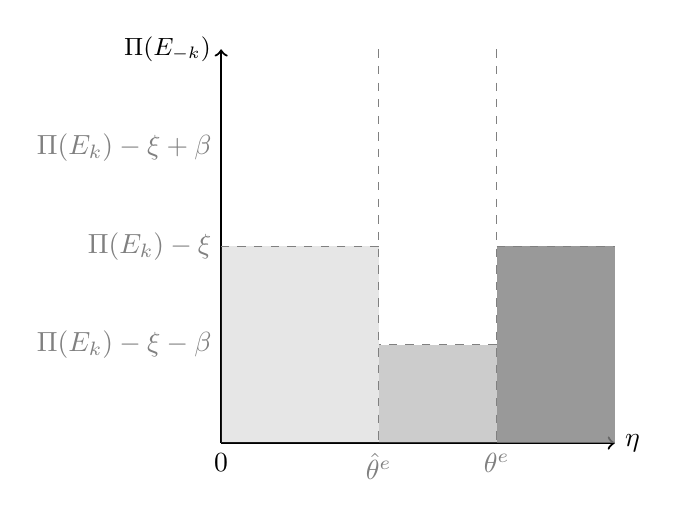
\begin{tikzpicture}
         \draw[black, thick][->] (0,0) -- (5,0) node[right] {$\eta$};
         \draw[black, thick][->] (0,0) node[below]{0} -- (0,5) node[left] {\small{$\Pi(E_{-k})$}};
         \draw[gray, dashed] (2,5) -- (2,0) node[below] {$\hat{\theta}^e$};
         \draw[gray, dashed] (3.5,5) -- (3.5,0) node[below] {$\theta^e$};
         
         \draw[gray, dashed] (3.5,1.25) -- (2,1.25);
         \draw[gray] (0, 1.25) node[left] {$\Pi(E_k)-\xi-\beta$};
         
         \draw[gray, dashed] (3.5, 2.5) -- (5,2.5) (2,2.5) -- (0,2.5) node[left] {$\Pi(E_k)-\xi$};
         
         \draw[gray] (0,3.75) node[left] {$\Pi(E_k)-\xi+\beta$};
         \draw[draw=gray, draw opacity=0, fill=gray, fill opacity=0.2] (2,0)--(0,0)--(0,2.5)--(2,2.5) -- cycle;
         
         \draw[draw=gray, draw opacity=0, fill=gray, fill opacity=0.4] (2,0)--(3.5,0)--(3.5,1.25)--(2,1.25) -- cycle;
         
         \draw[draw=gray, draw opacity=0, fill=gray, fill opacity=0.8] (5,0)--(3.5,0)--(3.5,2.5)--(5,2.5) -- cycle;
    \end{tikzpicture}}
\end{minipage}
\begin{minipage}{0.49\textwidth}
\centering
    Si $\theta^e < \hat{\theta}^e$

    \scriptsize{
    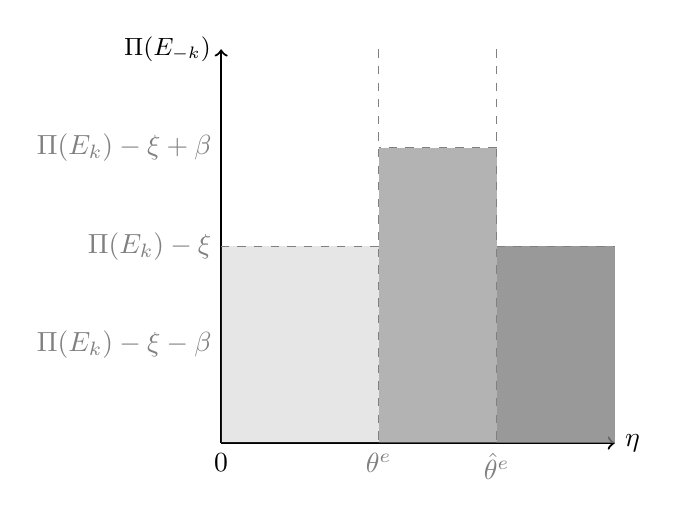
\begin{tikzpicture}
         \draw[black, thick][->] (0,0) -- (5,0) node[right] {$\eta$};
         \draw[black, thick][->] (0,0) node[below]{0} -- (0,5) node[left] {\small{$\Pi(E_{-k})$}};
         \draw[gray, dashed] (2,5) -- (2,0) node[below] {$\theta^e$};
         \draw[gray, dashed] (3.5,5) -- (3.5,0) node[below] {$\hat{\theta}^e$};
         
         \draw[gray, dashed] (3.5, 3.75) -- (2,3.75) ;
         \draw[gray] (0, 1.25) node[left] {$\Pi(E_k)-\xi-\beta$};
         
         \draw[gray, dashed] (3.5, 2.5) -- (5,2.5) (2,2.5) -- (0,2.5) node[left] {$\Pi(E_k)-\xi$};
         
         \draw[gray] (0,3.75) node[left] {$\Pi(E_k)-\xi+\beta$};
         \draw[draw=gray, draw opacity=0, fill=gray, fill opacity=0.2] (2,0)--(0,0)--(0,2.5)--(2,2.5) -- cycle;
         
         \draw[draw=gray, draw opacity=0, fill=gray, fill opacity=0.6] (2,0)--(3.5,0)--(3.5,3.75)--(2,3.75) -- cycle;
         
         \draw[draw=gray, draw opacity=0, fill=gray, fill opacity=0.8] (5,0)--(3.5,0)--(3.5,2.5)--(5,2.5) -- cycle;
    \end{tikzpicture}}
\end{minipage}
\begin{minipage}{\textwidth}
    \centering
    \vspace*{0.5cm}
    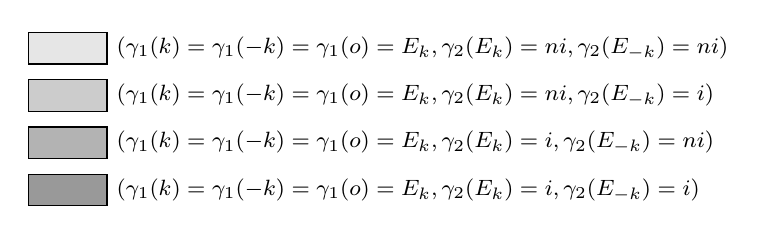
\begin{tikzpicture}
         \draw[draw=black, draw opacity=1, fill=gray, fill opacity=0.2] (1,1.8)--(0,1.8)--(0,2.2)--(1,2.2) -- cycle;
         \draw[black] (1,2) node[right] {\footnotesize{$(\gamma_1(k)=\gamma_1(-k)=\gamma_1(o)=E_k, \gamma_2(E_k)=ni, \gamma_2(E_{-k})=ni)$}};
         
         \draw[draw=black, draw opacity=1, fill=gray, fill opacity=0.4] (1,1.2)--(0,1.2)--(0,1.6)--(1,1.6) -- cycle;
         \draw[black] (1,1.4) node[right] {\footnotesize{$(\gamma_1(k)=\gamma_1(-k)=\gamma_1(o)=E_k, \gamma_2(E_k)=ni, \gamma_2(E_{-k})=i)$}};
         
         \draw[draw=black, draw opacity=1, fill=gray, fill opacity=0.6] (1,0.6)--(0,0.6)--(0,1)--(1,1) -- cycle;
         \draw[black] (1,0.8) node[right] {\footnotesize{$(\gamma_1(k)=\gamma_1(-k)=\gamma_1(o)=E_k, \gamma_2(E_k)=i, \gamma_2(E_{-k})=ni)$}};
         
         \draw[draw=black, draw opacity=1, fill=gray, fill opacity=0.8] (1,0)--(0,0)--(0,0.4)--(1,0.4) -- cycle;
         \draw[black] (1,0.2) node[right] {\footnotesize{$(\gamma_1(k)=\gamma_1(-k)=\gamma_1(o)=E_k, \gamma_2(E_k)=i, \gamma_2(E_{-k})=i)$}};
         
    \end{tikzpicture}
\end{minipage}
\begin{singlespace}
    \floatfoot{\footnotesize{\textit{Nota:} La figura representa los equilibrios agrupadores del modelo. $\beta$ es el costo que percibe el jugador 1 de no interactuar con el jugador 2. $\xi$ es el costo de violar uno mismo la norma social. $\eta$ es el costo que percibe el jugador 2 de no interactuar con el jugador 1, $\theta^e$ es el costo esperado por el jugador 2 de que el jugador 1 esté violando la norma social y $\hat{\theta}^e$ el costo esperado por el jugador 2 fuera de la senda de equilibrio de que el jugador 1 esté violando la norma social.}\par}
\end{singlespace}

\label{fig:equilibriosagru}
\end{figure}





    \section{Descriptivas}
\begin{table}[ht!]
        \centering
        \caption{Estadísticas descriptivas}
        \footnotesize{
        \begin{tabular}{l ccc c}\hline \hline
                &\multicolumn{1}{c}{Total}&\multicolumn{1}{c}{Masculinos}&\multicolumn{1}{c}{Femeninos}&\multicolumn{1}{c}{Dif (2)-(3)}\\\hline
                &\multicolumn{1}{c}{(1)}&\multicolumn{1}{c}{(2)}&\multicolumn{1}{c}{(3)}&\multicolumn{1}{c}{(4)}\\
            Edad      &    20.15&    20.25&    20.05&     0.20         \\
                            &  (1.710)&  (1.832)&  (1.589)&  [0.324]         \\
            Bogotá=1          &     0.59&     0.66&     0.52&     0.14         \\
                            &  (0.494)&  (0.478)&  (0.504)&  [0.093]         \\
            Semestres &     6.18&     5.96&     6.39&    -0.43         \\
                            &  (2.935)&  (3.057)&  (2.820)&  [0.556]         \\
            Apoyo financiero&     0.68&     0.61&     0.75&    -0.14         \\
                            &  (0.469)&  (0.493)&  (0.437)&  [0.088]         \\
                             &          &       &           &               \\
            Observaciones    &      112&       56&       56&      112         \\\hline \hline

        \end{tabular}}
        \begin{threeparttable} 
        \begin{tablenotes}
        \footnotesize{
        \item \textit{Nota}: Estadísticas descriptivas de los participantes del experimento. Desviaciones estándar en paréntesis. Errores estándares en corchetes; *** p$<$0.01, ** p$<$0.05, * p$<$0.1.}
        \end{tablenotes}
        \end{threeparttable}
    \end{table}

\subsection{Validación de norma social de habilidad}
\FloatBarrier 
\begin{figure}[ht!]
    \centering
    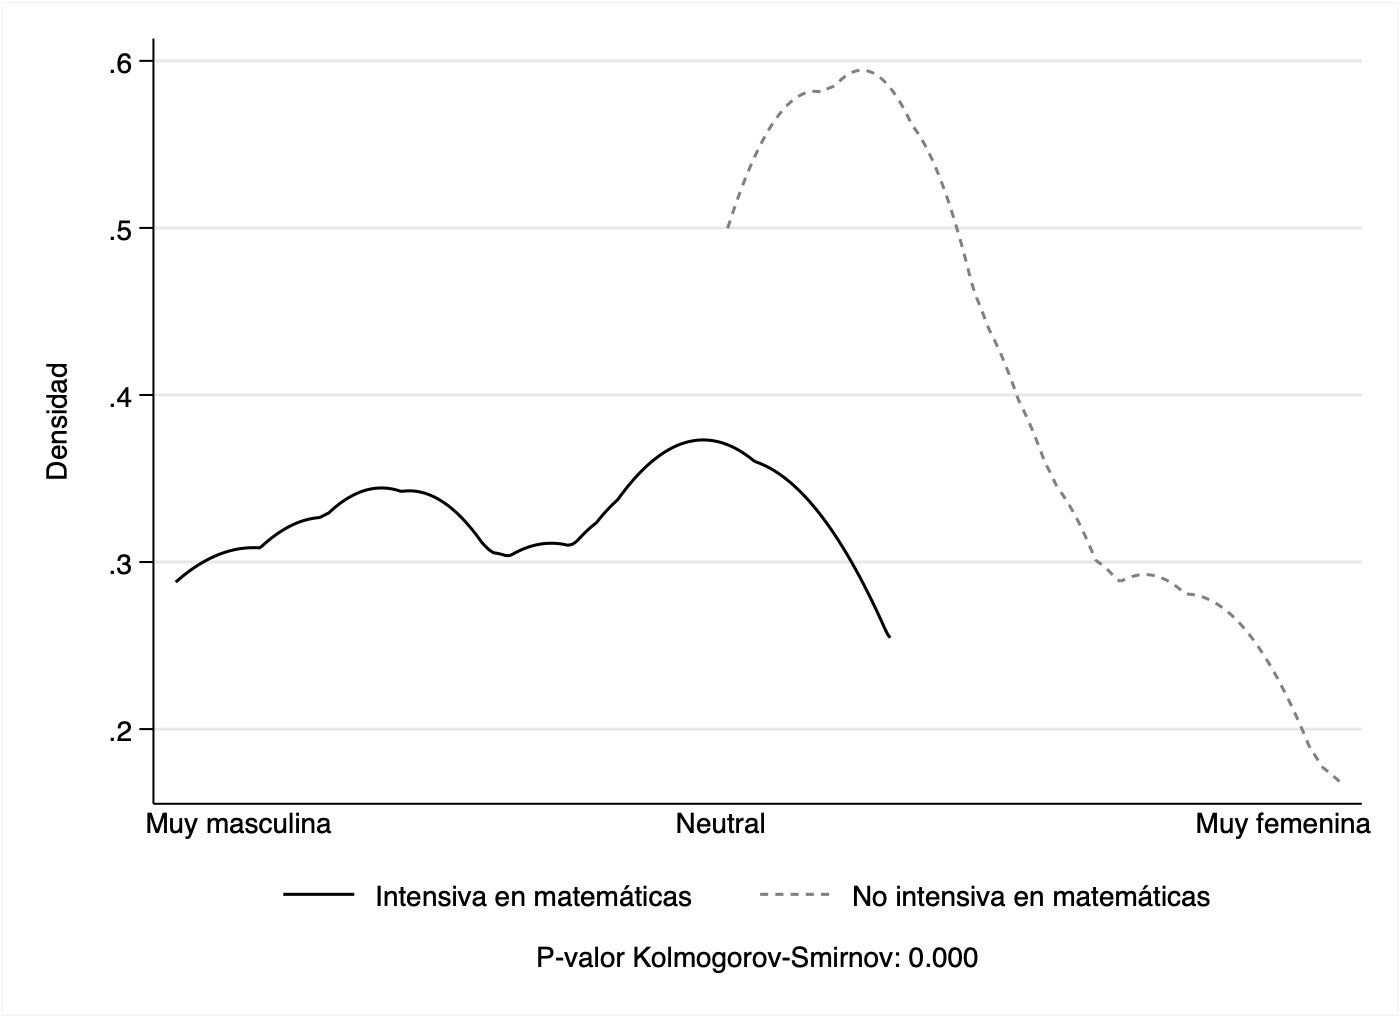
\includegraphics[width=12cm]{Images/career_perception.png}
    \caption{Percepción de carreras}
    \label{fig:careers}
    \begin{singlespace}
    \floatfoot{\footnotesize{\textit{Nota:} Gráfica de la percepción de 30 carreras clasificadas de 1 a 9 de muy masculina a muy femenina. La clasificación promedio hecha por una muestra de estudiantes, diferentes a los participantes del experimento. Las carreras son clasificadas como intensivas en matemáticas si tienen dos o más clases de matemáticas en su pensum, y como no intensivas de lo contrario.}\par}
    \end{singlespace}
\end{figure}


\subsection{Distribución de expresiones de género}
\FloatBarrier 
\begin{table}[ht]
    \centering
    \caption{Distribución por género de vestimenta, habilidades y aspiraciones}
    \label{tab:distribuciones_expresiones}
    \begin{subtable}{\textwidth}
        \centering
        \caption{Identidad masculina}
        \vspace*{-0.5cm}
        \fontsize{9.5}{12}\selectfont {
        \begin{tabular}{cccccc} \\ \hline \hline
                                & \multicolumn{2}{c}{Puntaje vestimenta $<$ 0} & & \multicolumn{2}{c}{Puntaje vestimenta $>$ 0} \\\cmidrule{2-3} \cmidrule{5-6}
                                & \textit{Económica}  & \textit{Familiar}      & &  \textit{Económica} & \textit{Familiar}      \\
        \textit{Matemáticas}    & 15                  & 11                     & & 1                   & 1                      \\
        \textit{Comunicación}   & 15                  & 11                     & & 1                   & 1                      \\\hline \hline
        \end{tabular}}
    \end{subtable}
    \begin{minipage}{\textwidth}
    \hspace*{2cm}
    \end{minipage}
    \begin{subtable}{\textwidth}
        \centering
        \vspace*{0.5cm}
        \caption{Identidad femenina}
        \vspace*{-0.5cm}
        \fontsize{9.5}{12}\selectfont {
        \begin{tabular}{cccccc}\\ \hline \hline
                                & \multicolumn{2}{c}{Puntaje vestimenta $<$ 0} & & \multicolumn{2}{c}{Puntaje vestimenta $>$ 0} \\\cmidrule{2-3} \cmidrule{5-6}
                                & \textit{Económica}  & \textit{Familiar}      & &  \textit{Económica} & \textit{Familiar}      \\
        \textit{Matemáticas}    & 1                   & 0                      & & 7                   & 5                      \\
        \textit{Comunicación}   & 1                   & 4                      & & 20                  & 18                     \\\hline \hline
        \end{tabular}}
    \end{subtable}
    \begin{threeparttable} 
    \begin{tablenotes}
    \footnotesize{
    \item Nota: Las tablas contienen la cantidad de participantes con esas características, discriminado por la identidad de género que reportó cada participante en la inscripción. Un puntaje de vestimenta $<\ 0$ representa una vestimenta más masculina que el promedio, un puntaje de vestimenta $>\ 0$ representa una vestimenta más femenina que el promedio. En las columnas están representadas la vestimenta y la aspiración, que es económica o familiar. Las filas representan la habilidad, que es matemáticas o comunicación.}
    \end{tablenotes}
    \end{threeparttable}
\end{table}

\FloatBarrier 
\begin{figure}[!ht]
	\centering
	\caption{Distribución vestimenta}
	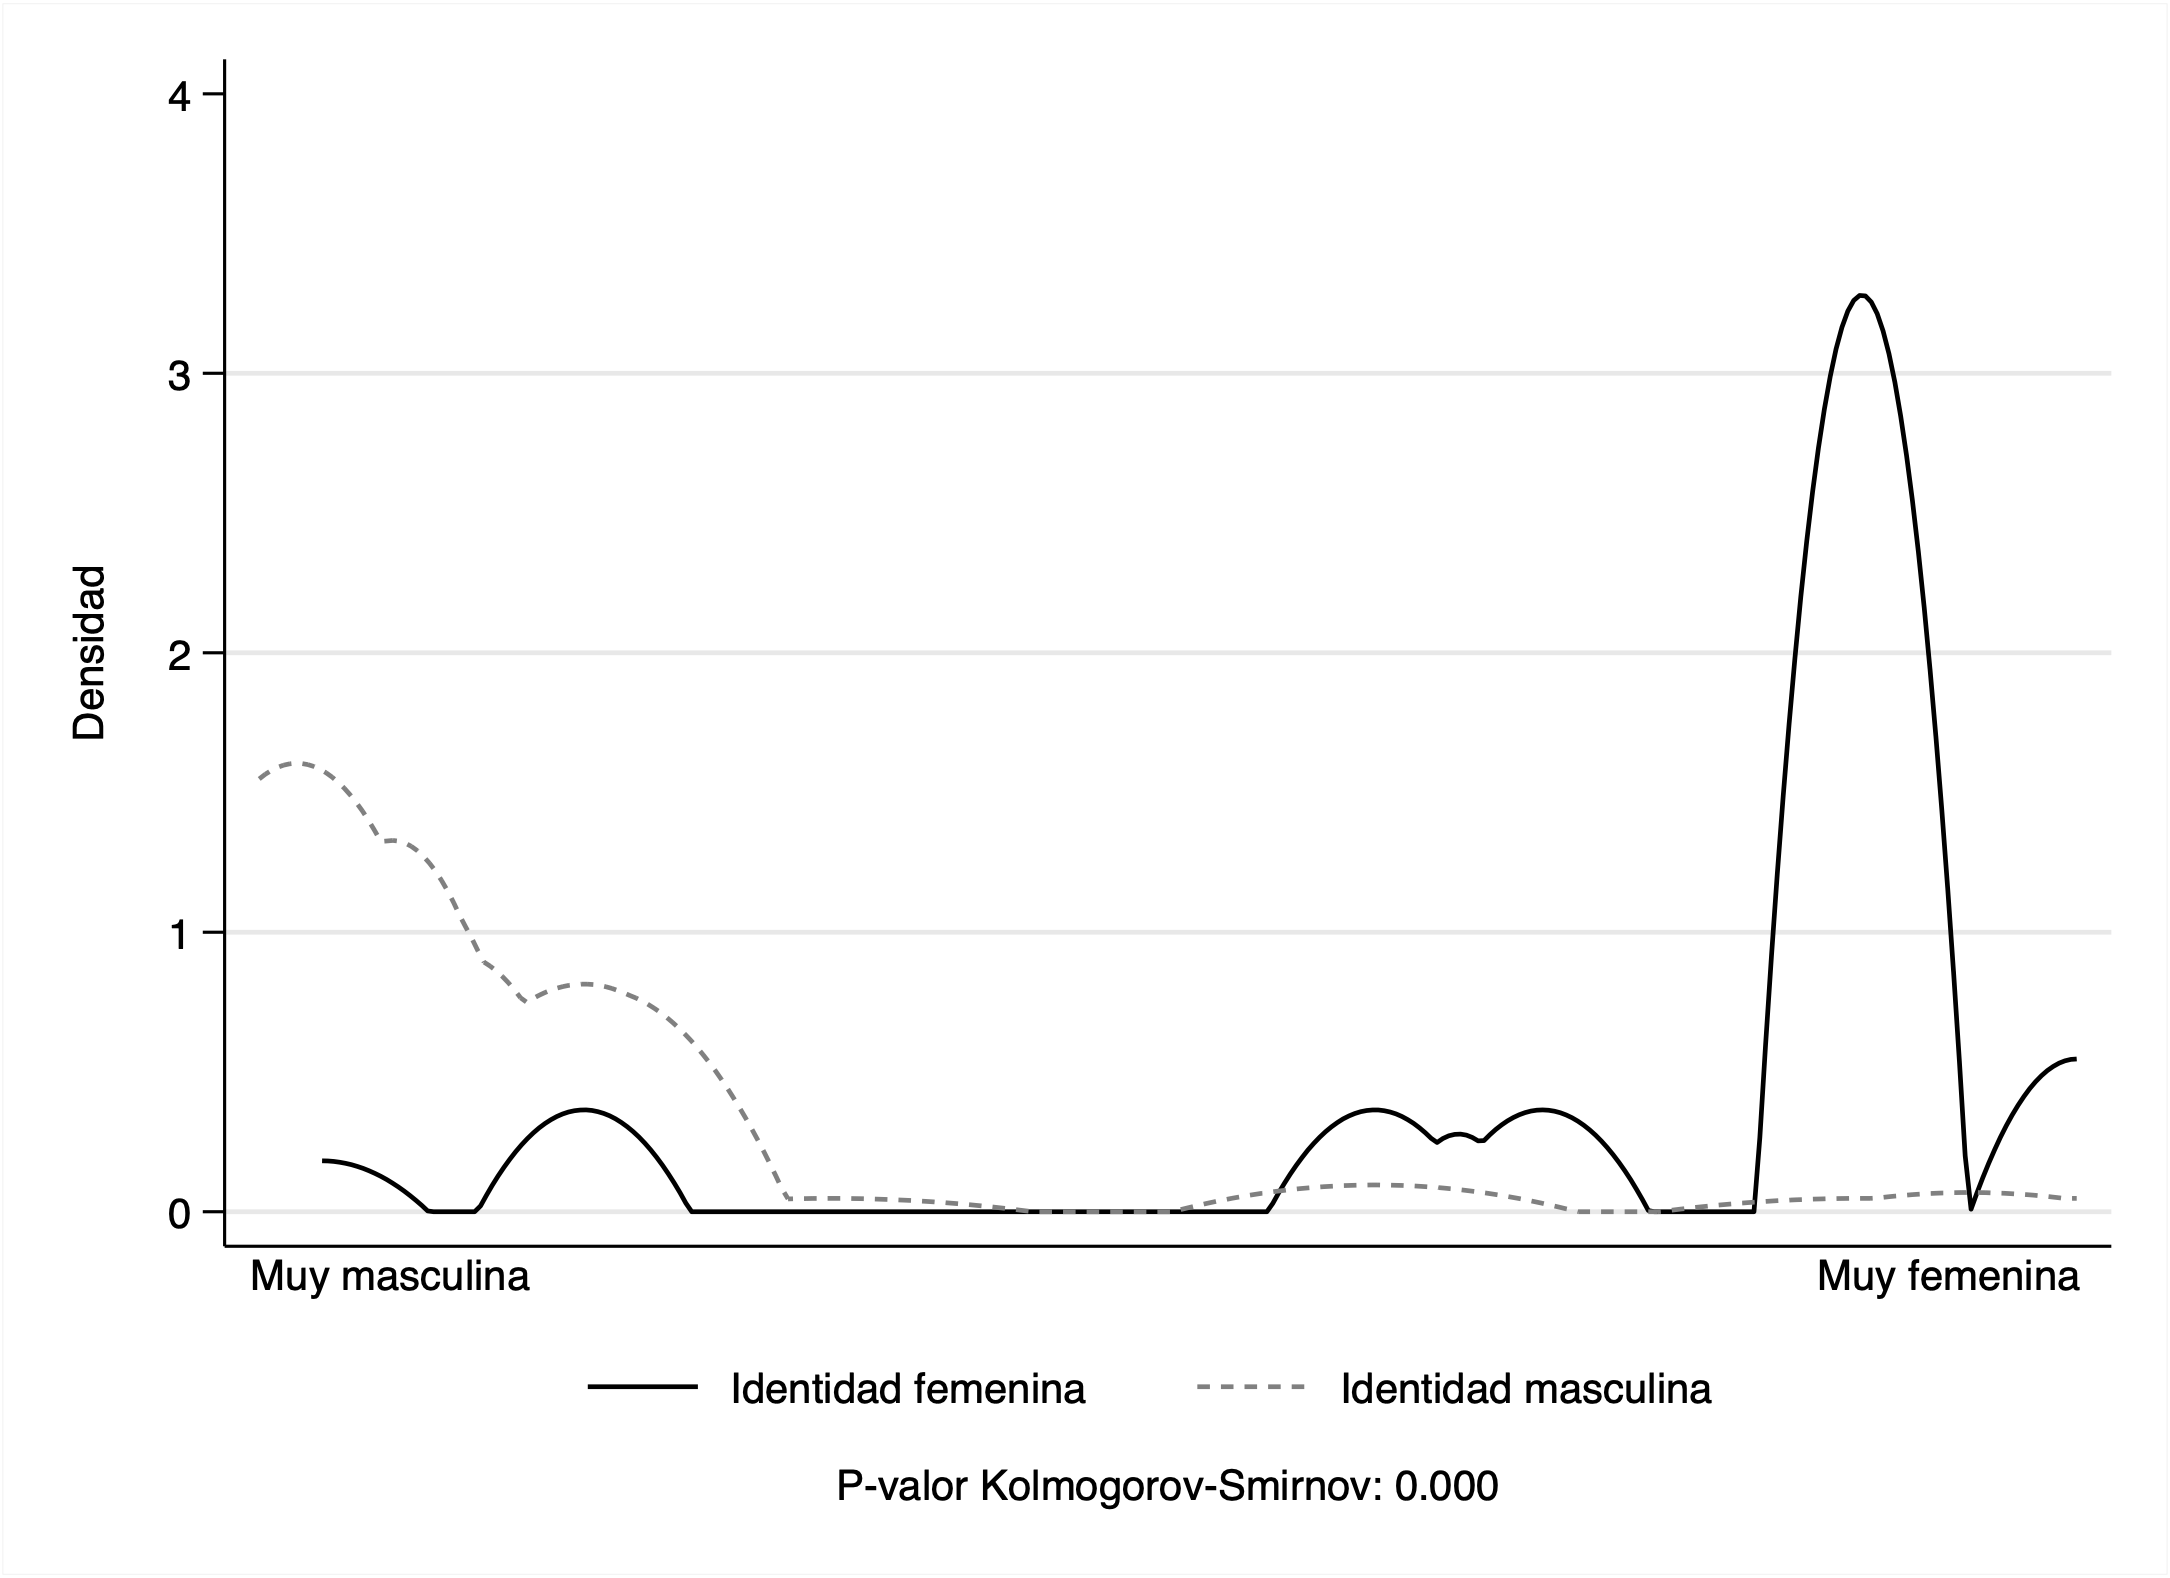
\includegraphics[width=13cm]{Images/dress_score_gender.png}
	\label{fig:dress_dist}
	\begin{singlespace}
    \floatfoot{\footnotesize{\textit{Nota:} Distribución del puntaje de vestimenta entre las vestimentas elegidas por los participantes del experimento. Prueba Kolmogorov-Smirnov de diferencia en la distribución por género.}\par}
    \end{singlespace}
\end{figure}
\begin{figure}[!ht]
	\centering
	\caption{Distribución habilidad}
	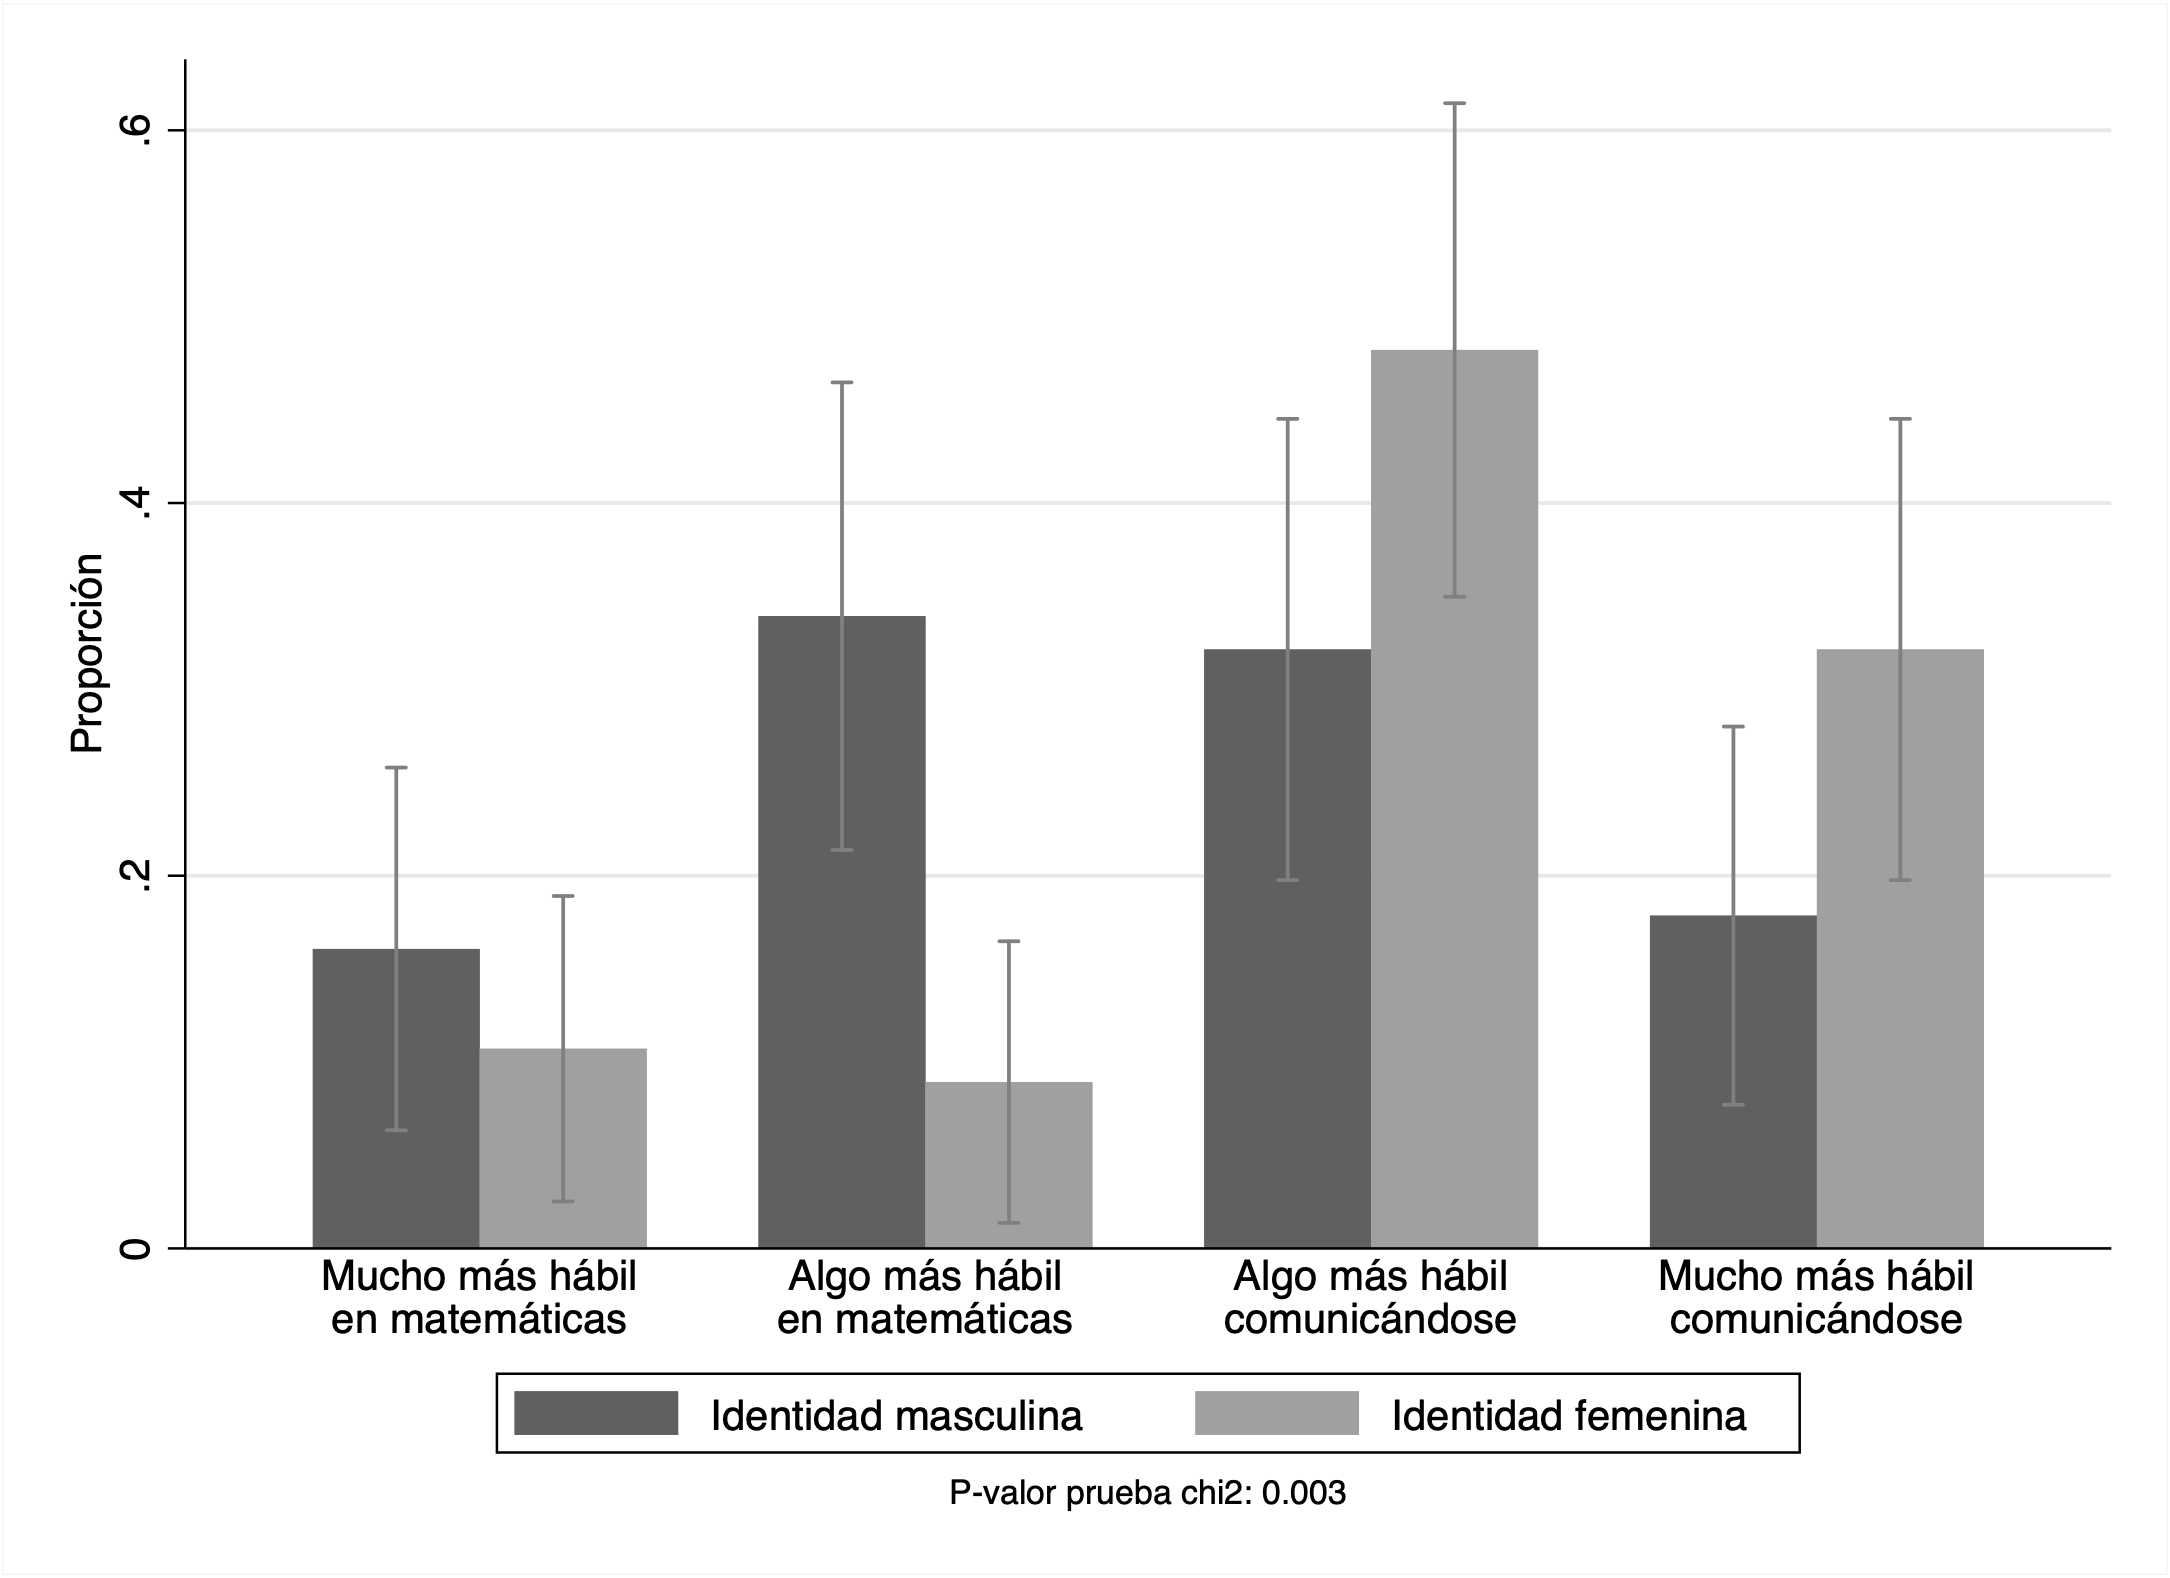
\includegraphics[width=12cm]{Images/ability_likert.png}
	\label{fig:ability_dist}
	\begin{singlespace}
    \floatfoot{\footnotesize{\textit{Nota:} Gráfica de respuestas de participante a la escala de likert sobre su principal habilidad, entre comunicación y matemáticas. Prueba chi2 de diferencia en género de indicador de si participante reportó ser más hábiles comunicándose que en matemáticas.}\par}
    \end{singlespace}
\end{figure}
\begin{figure}[!ht]
	\centering
	\caption{Distribución aspiraciones- reportada en escala de likert}
	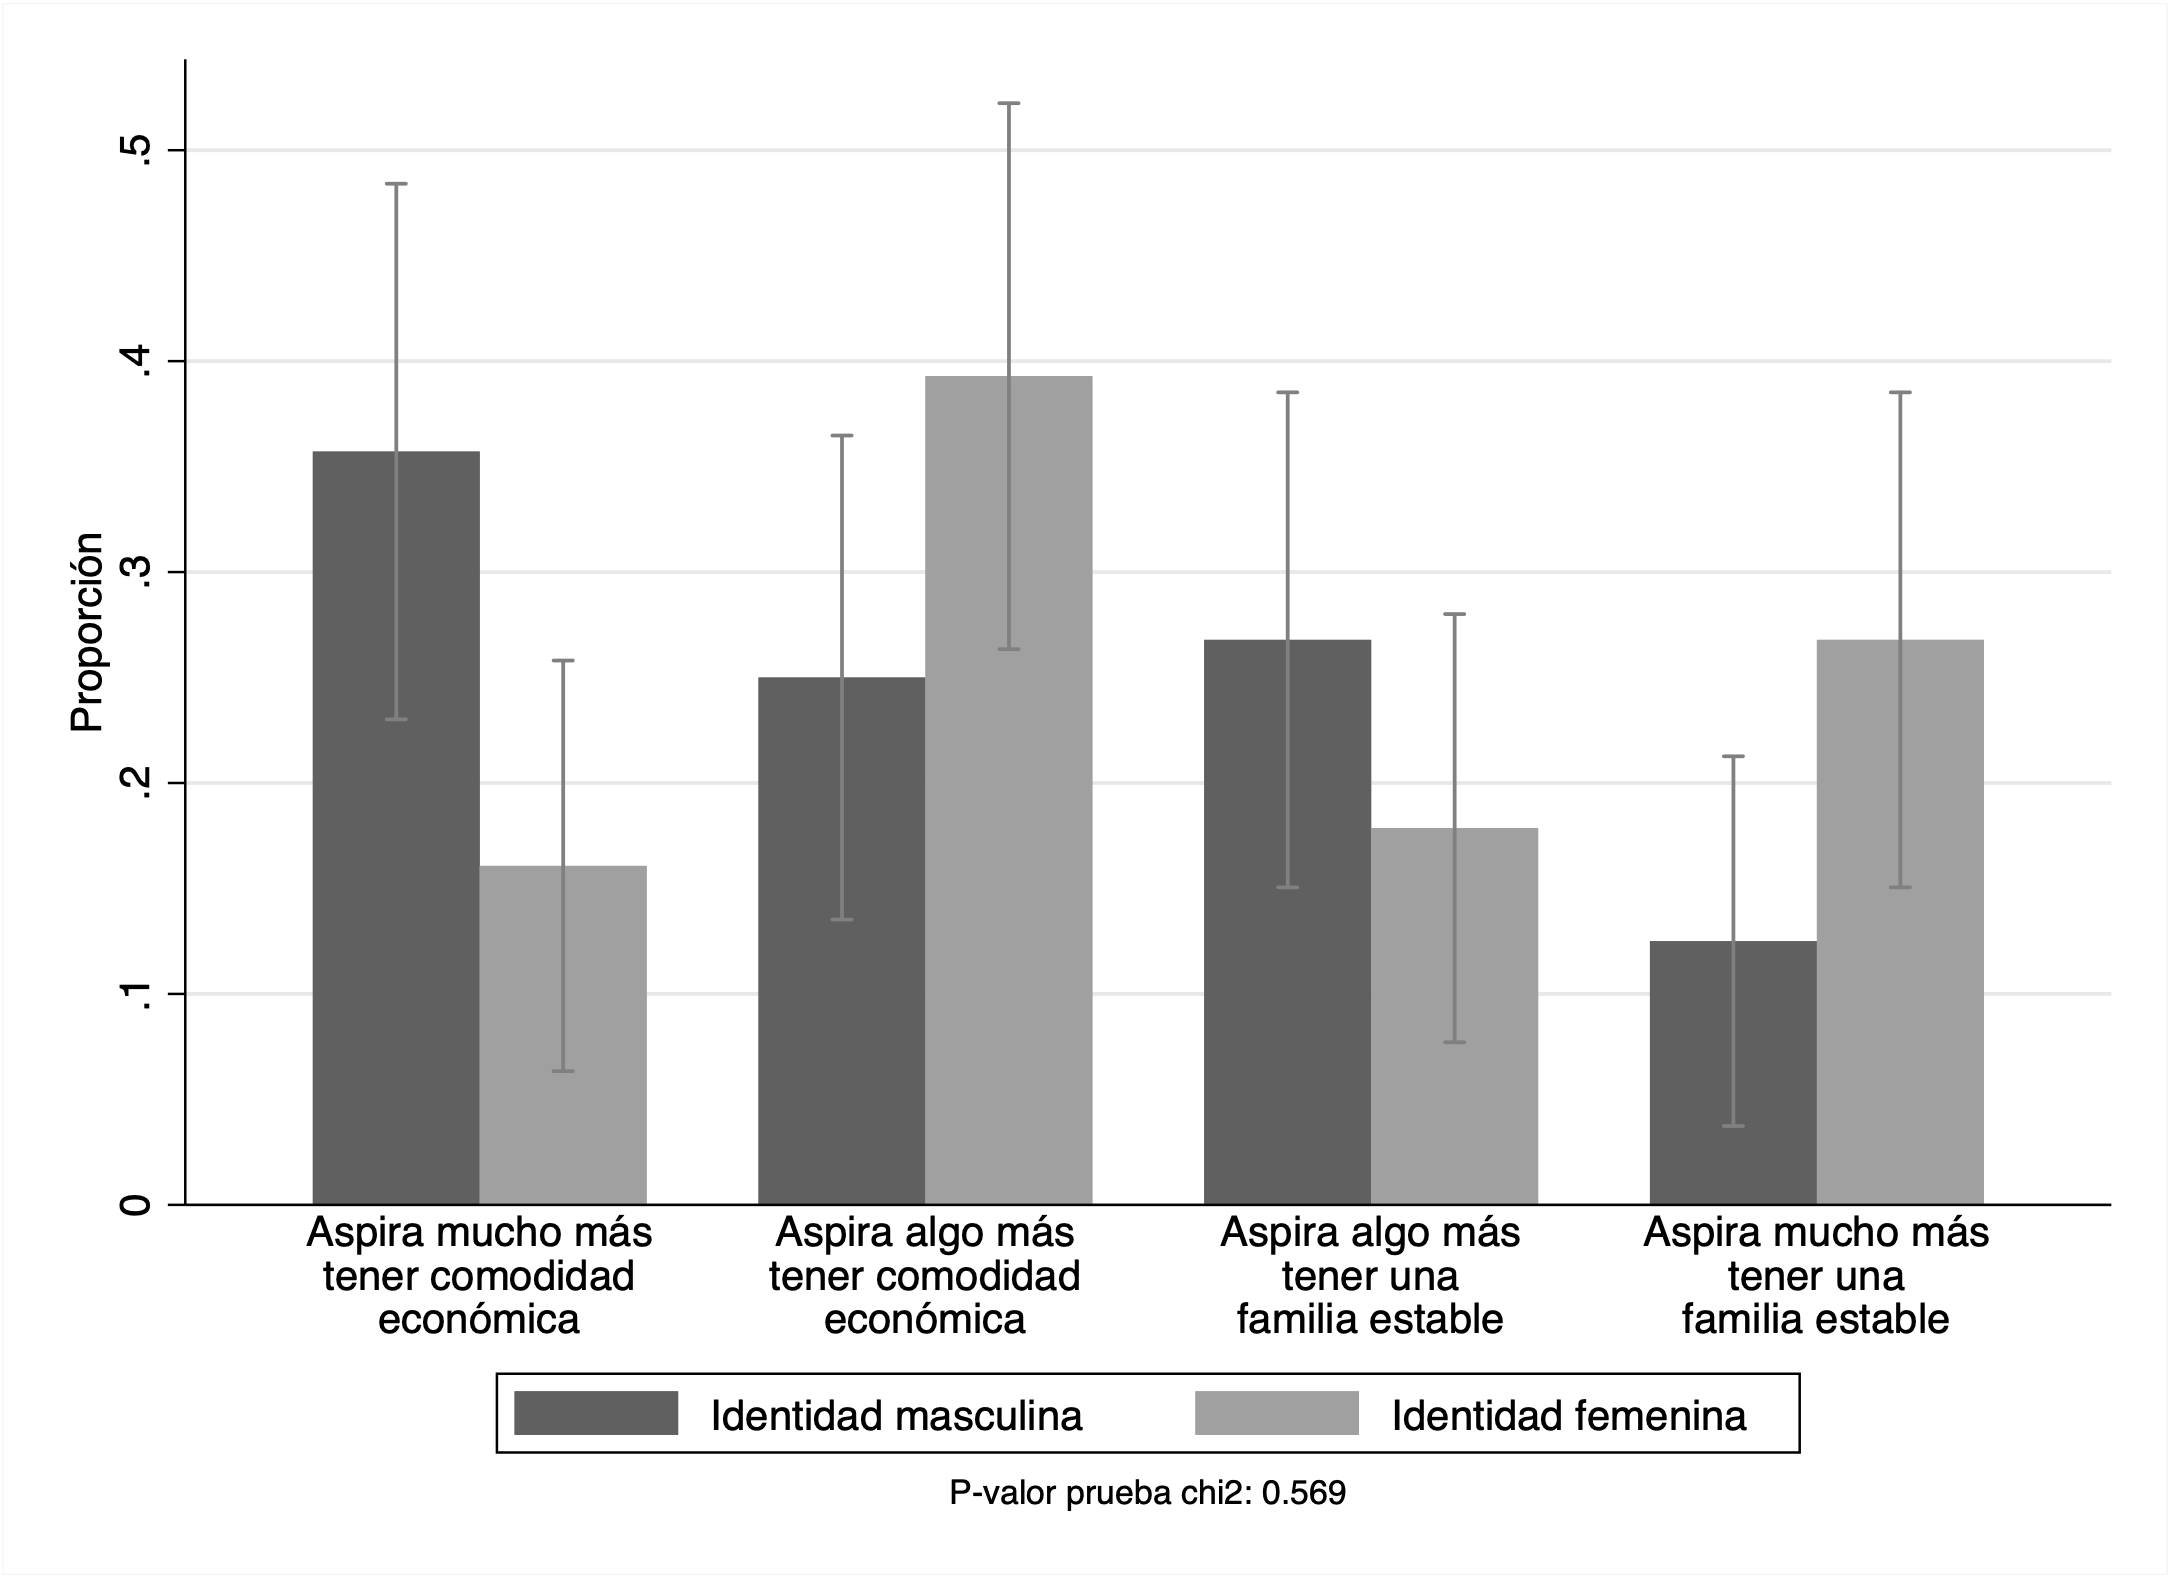
\includegraphics[width=12cm]{Images/aspiration_likert.png}
	\label{fig:aspiration_dist}
	\begin{singlespace}
    \floatfoot{\footnotesize{\textit{Nota:} Gráfica de respuestas de participante a la escala de likert sobre su aspiración principal, entre estabilidad familiar y estabilidad económica. Prueba chi2 de diferencia en género de indicador de si participante reportó aspirar más a tener estabilidad familiar que estabilidad económica.}\par}
    \end{singlespace}
\end{figure}
\begin{figure}[!ht]
	\centering
	\caption{Distribución de expresiones de género }
	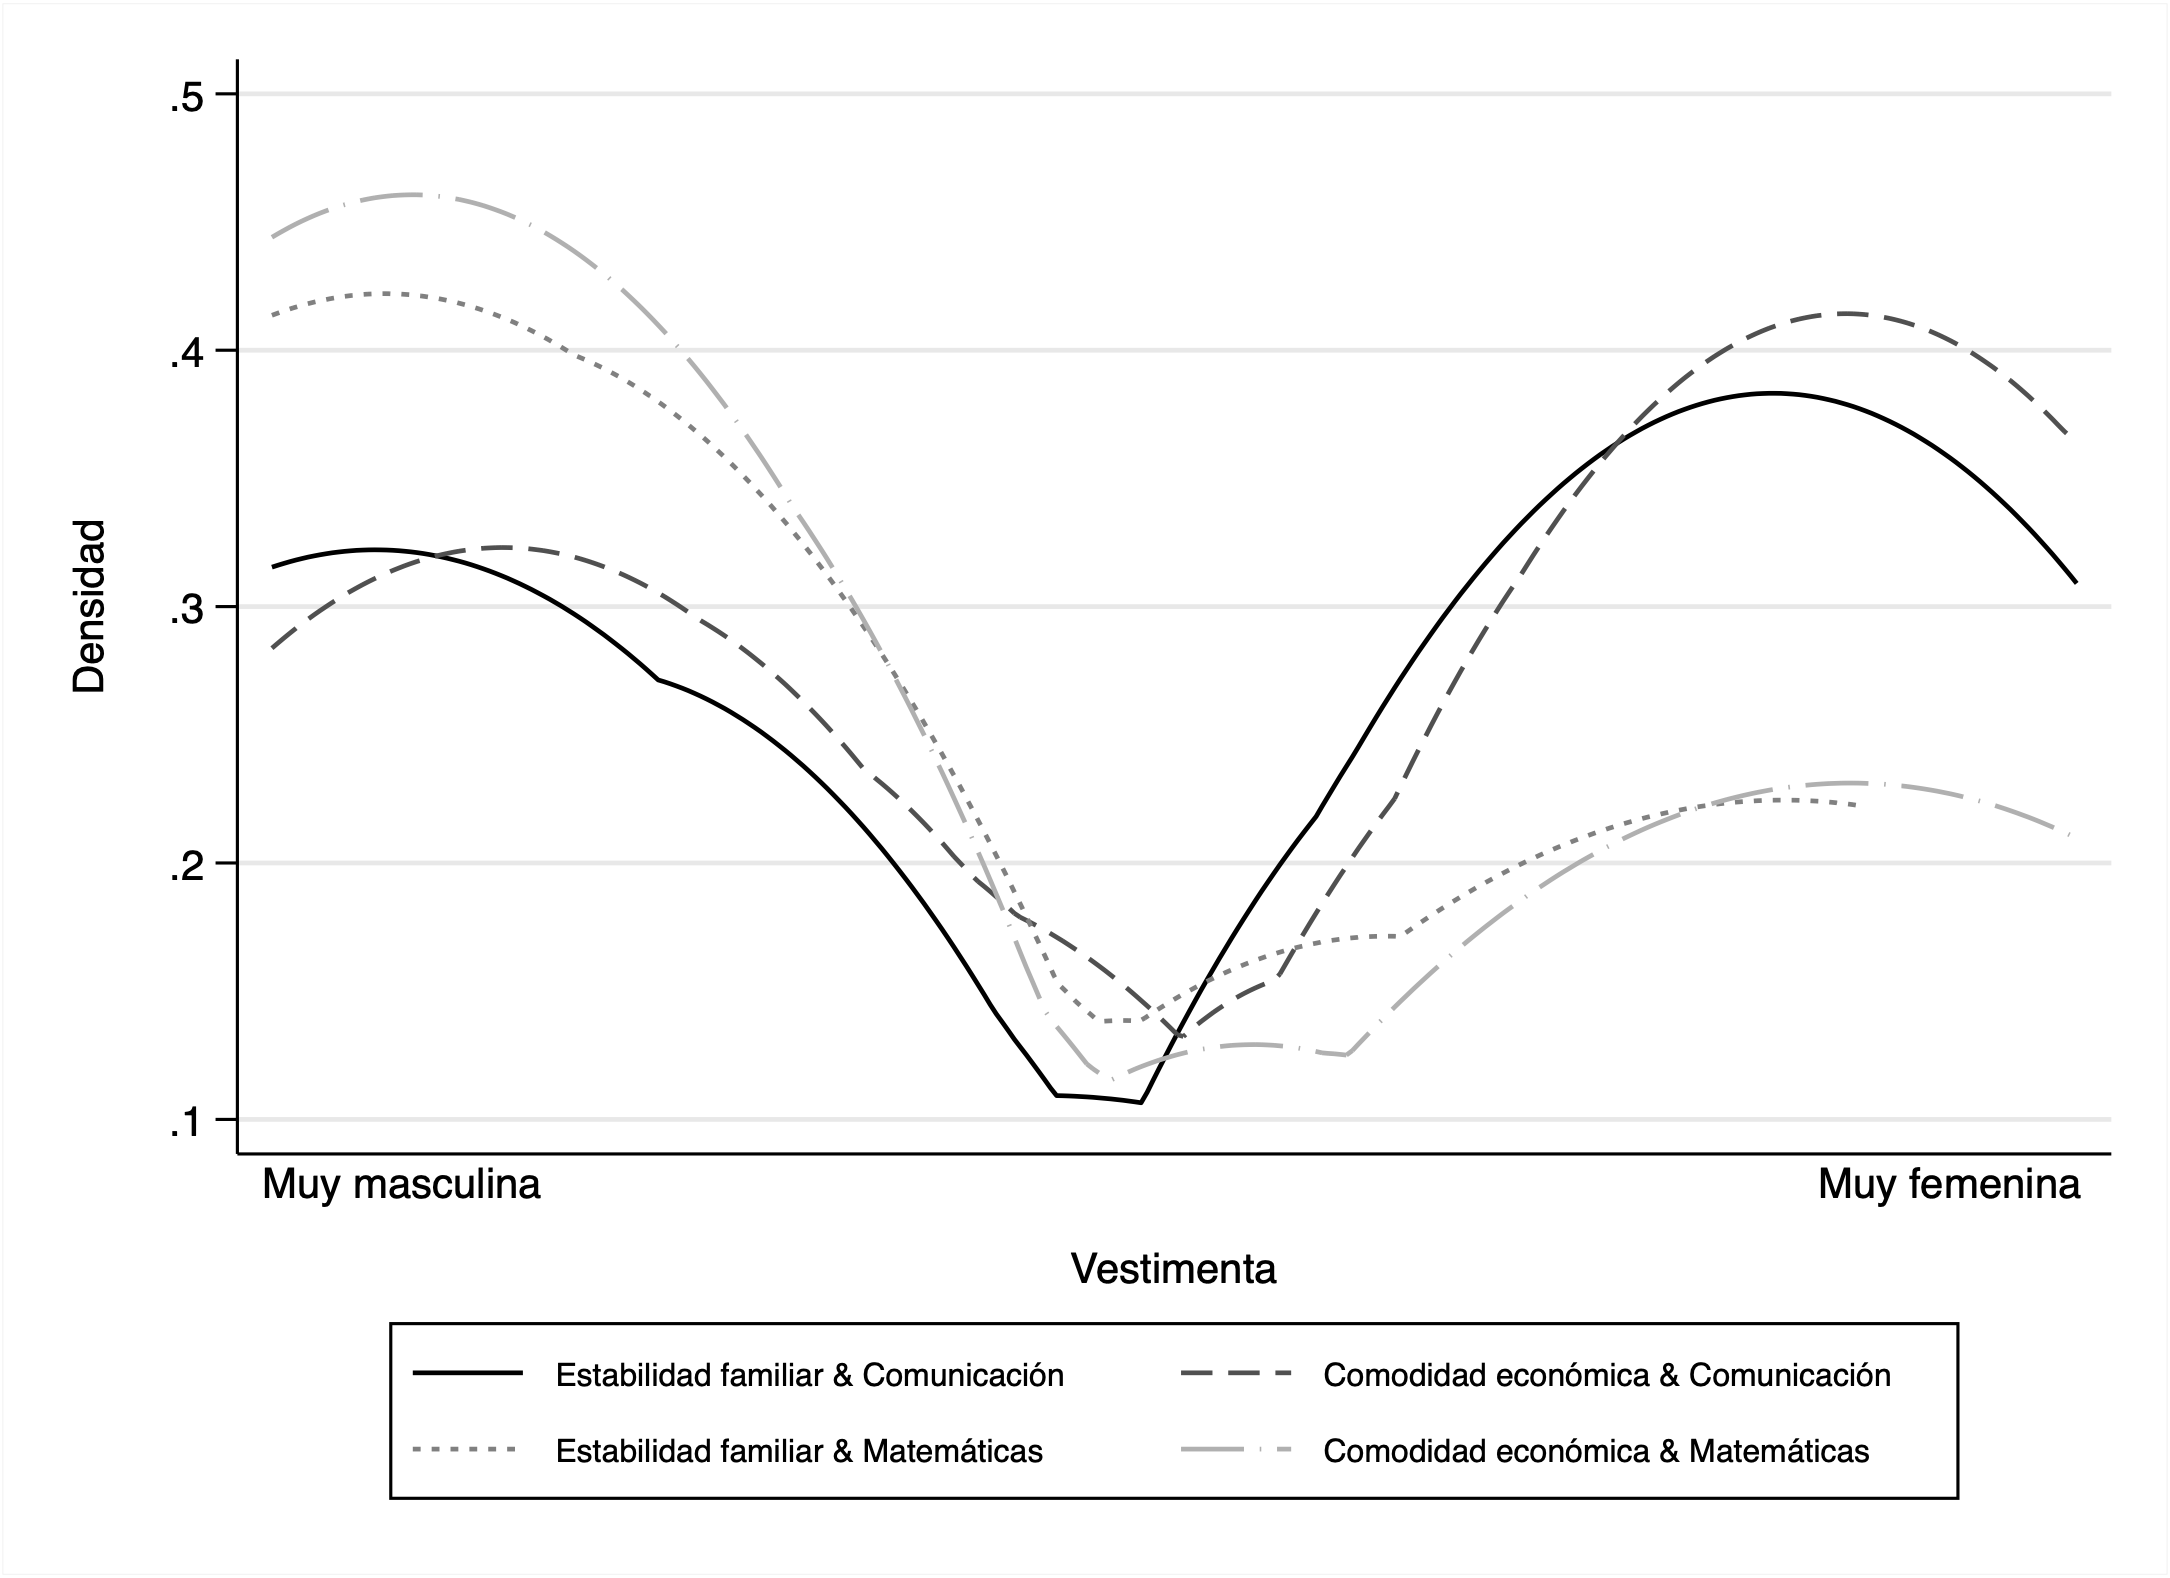
\includegraphics[width=12cm]{Images/gender_expressions.png}
	\label{fig:jointdistribution}
	\begin{singlespace}
    \floatfoot{\footnotesize{\textit{Nota:} Distribución por conjunto de expresiones de género.}\par}
    \end{singlespace}
\end{figure}
\vspace*{6cm}
    \section{Estimaciones alternativas}
\begin{table}[ht!]
    \centering
    \caption{Logit rankeado y ordenado}
    \label{tab:rol}
    \begin{threeparttable} \fontsize{8.5}{12}\selectfont {
    \begin{tabular}{lccc} \hline \hline
                                                & \multicolumn{3}{c}{Ranker}        \\\cmidrule{2-4}
                                                &   Todos   &  Femenino & Masculino \\ 
                                                &   (1)     &    (2)    &   (3)     \\ \hline
                                                &           &           &           \\
    Puntaje vestimenta  	                    &	-0.111	&	-0.280*	&	0.006	\\
                                        	    &  	(0.112)	&	(0.164)	&	(0.153)	\\
    Habilidad comunicación  	                &	0.225	&	0.394*	&	0.058	\\
    	                                        &	(0.151)	&	(0.234)	&	(0.190)	\\
    Habilidad comunicación*Puntaje vestimenta 	&	0.132	&	0.246	&	0.100	\\
                                            	&	(0.124)	&	(0.193)	&	(0.176)	\\
    Aspiración familiar 	                    &	0.141	&	0.339*	&	-0.024	\\
    	                                        &	(0.142)	&	(0.203)	&	(0.216)	\\
    Edad	                                    &	-0.026	&	-0.049	&	-0.015	\\
    	                                        &	(0.038)	&	(0.056)	&	(0.056)	\\
    Bogotá = 1	                                &	-0.032	&	-0.035	&	-0.041	\\
                                            	&	(0.146)	&	(0.242)	&	(0.180)	\\
    Posición Inicial	                        &. 0.156*** & 0.171***	& 0.146***	\\
    	                                        &	(0.031)	&	(0.044)	&	(0.044)	\\

                                                &           &           &           \\
    Observaciones                               &   560     &   264     &   296     \\
    Número de rankers                           &   70      &   33      &   37      \\ \hline \hline
    \end{tabular}}
    \begin{tablenotes}
    \footnotesize{
    \item \textit{Nota:} Estimaciones por logit rankeado y ordenado del efecto de las expresiones de género en el ranking que recibieron por parte de sus pares. Puntaje vestimenta es el puntaje estandarizado de qué tan femenina se percibe la vestimenta que se observa. Habilidad comunicación es el indicador que toma el valor de uno si se observa que el par es más hábil comunicándose que en matemáticas. Aspiración familiar es el indicador que toma el valor de uno si se observa que el par aspira más a formar familia que a tener comodidad económica. Edad es la edad del par que se observa. Bogotá es un indicador que toma el valor de uno si el par que se observa nació en Bogotá, y posición inicial es la posición que ocupaba el par en el listado antes de que los perfiles fueran organizados. 
    \item Errores estándares robustos en paréntesis; *** p$<$0.01, ** p$<$0.05, * p$<$0.1.}
    \end{tablenotes}
    \end{threeparttable}
\end{table}

\begin{table}[ht!]
    \centering
    \caption{Ranking promedio}
    \label{tab:mean}
    \begin{threeparttable} \fontsize{8.5}{12}\selectfont {
    \begin{tabular}{lccc} \hline \hline
                                                & \multicolumn{3}{c}{Ranker}        \\\cmidrule{2-4}
                                                &   Todos   &  Femenino & Masculino \\ 
                                                &   (1)     &    (2)    &   (3)     \\ \hline
                                                &           &           &           \\
    Puntaje vestimenta                      	&	-0.101	&	-0.234	&	0.034	\\
                                            	&	(0.168)	&	(0.283)	&	(0.242)	\\
    Habilidad comunicación  	                &	0.479**	&	0.470	&	0.332	\\
    	                                        &	(0.209)	&	(0.321)	&	(0.308)	\\
    Habilidad comunicación*Puntaje vestimenta 	&	0.141	&	0.189	&	-0.026	\\
                                            	&	(0.232)	&	(0.349)	&	(0.328)	\\
    Aspiración familiar 	                    &	0.196	&	0.600*	&	0.006	\\
                                            	&	(0.206)	&	(0.310)	&	(0.303)	\\
    Edad	                                    &	0.001	&	-0.006	&	0.031	\\
                                            	&	(0.061)	&	(0.100)	&	(0.102)	\\
    Bogotá = 1	                                &	-0.045	&	-0.115	&	-0.086	\\
    	                                        &	(0.212)	&	(0.328)	&	(0.304)	\\
    Posición Inicial	                        &	0.264**	& 0.367***	&	0.237*	\\
    	                                        &	(0.123)	&	(0.107)	&	(0.127)	\\
    Constante	                                &	2.933*	&	2.422	&	2.710	\\
    	                                        &	(1.561)	&	(2.082)	&	(2.330)	\\
    	                                        &		    &		    &		    \\
    Observaciones	                            &	113	    &	110	    &	112	    \\\hline \hline
    \end{tabular}}
    \begin{tablenotes}
    \footnotesize{
    \item \textit{Nota:} Estimaciones por mínimos cuadrados ordinarios del efecto de las expresiones de género en el promedio de rankings. Puntaje vestimenta es el puntaje estandarizado de qué tan femenina se percibe la vestimenta que se observa. Habilidad comunicación es el indicador que toma el valor de uno si se observa que el par es más hábil comunicándose que en matemáticas. Aspiración familiar es el indicador que toma el valor de uno si se observa que el par aspira más a formar familia que a tener comodidad económica. Edad es la edad del par que se observa. Bogotá es un indicador que toma el valor de uno si el par que se observa nació en Bogotá, y posición inicial es el promedio de las posiciones que ocupaba el par en los listados antes de que los perfiles fueran organizados. 
    \item Errores estándares robustos en paréntesis; *** p$<$0.01, ** p$<$0.05, * p$<$0.1.}
    \end{tablenotes}
    \end{threeparttable}
\end{table}

  
    \section{Cálculos de poder}
Este experimento cuenta con estrictamente con 36 tratamientos si la combinación de cada vestimenta, con cada habilidad y cada aspiración es considerada un tratamiento. Si en cambio las vestimentas son agrupadas en tres categorías (femenina, masculina y ambigua/neutral), el experimento tiene 8 tratamientos. Los siguientes cálculos de poder supone son 8 tratamientos. 

Para detectar un efecto de 0.15d,e con un nivel de significancia de 0.05, con un poder del 80\% es necesario tener una muestra de $1,396$ por tratamiento (ver Figura \ref{fig:calc} ). Es decir, en total era necesario tener una muestra de $11,168$ para tener 80\% de poder para ver efectos de 0.15d.e. Para ver efectos de 0.3d.e con una significancia de 0.05 y un poder del 80\% era necesario tener en total un muestra de $2,792$ (ver Figura \ref{fig:calc}). Ahora, con la muestra de este trabajo el poder para detectar efectos de 0.15d.e es del 10\% y para detectar efectos de 0.3d.e es de 25\%.

\begin{figure}[!ht]
    \centering
    \caption{Cálculos de poder}
    \begin{subfigure}{\textwidth}
        \centering
        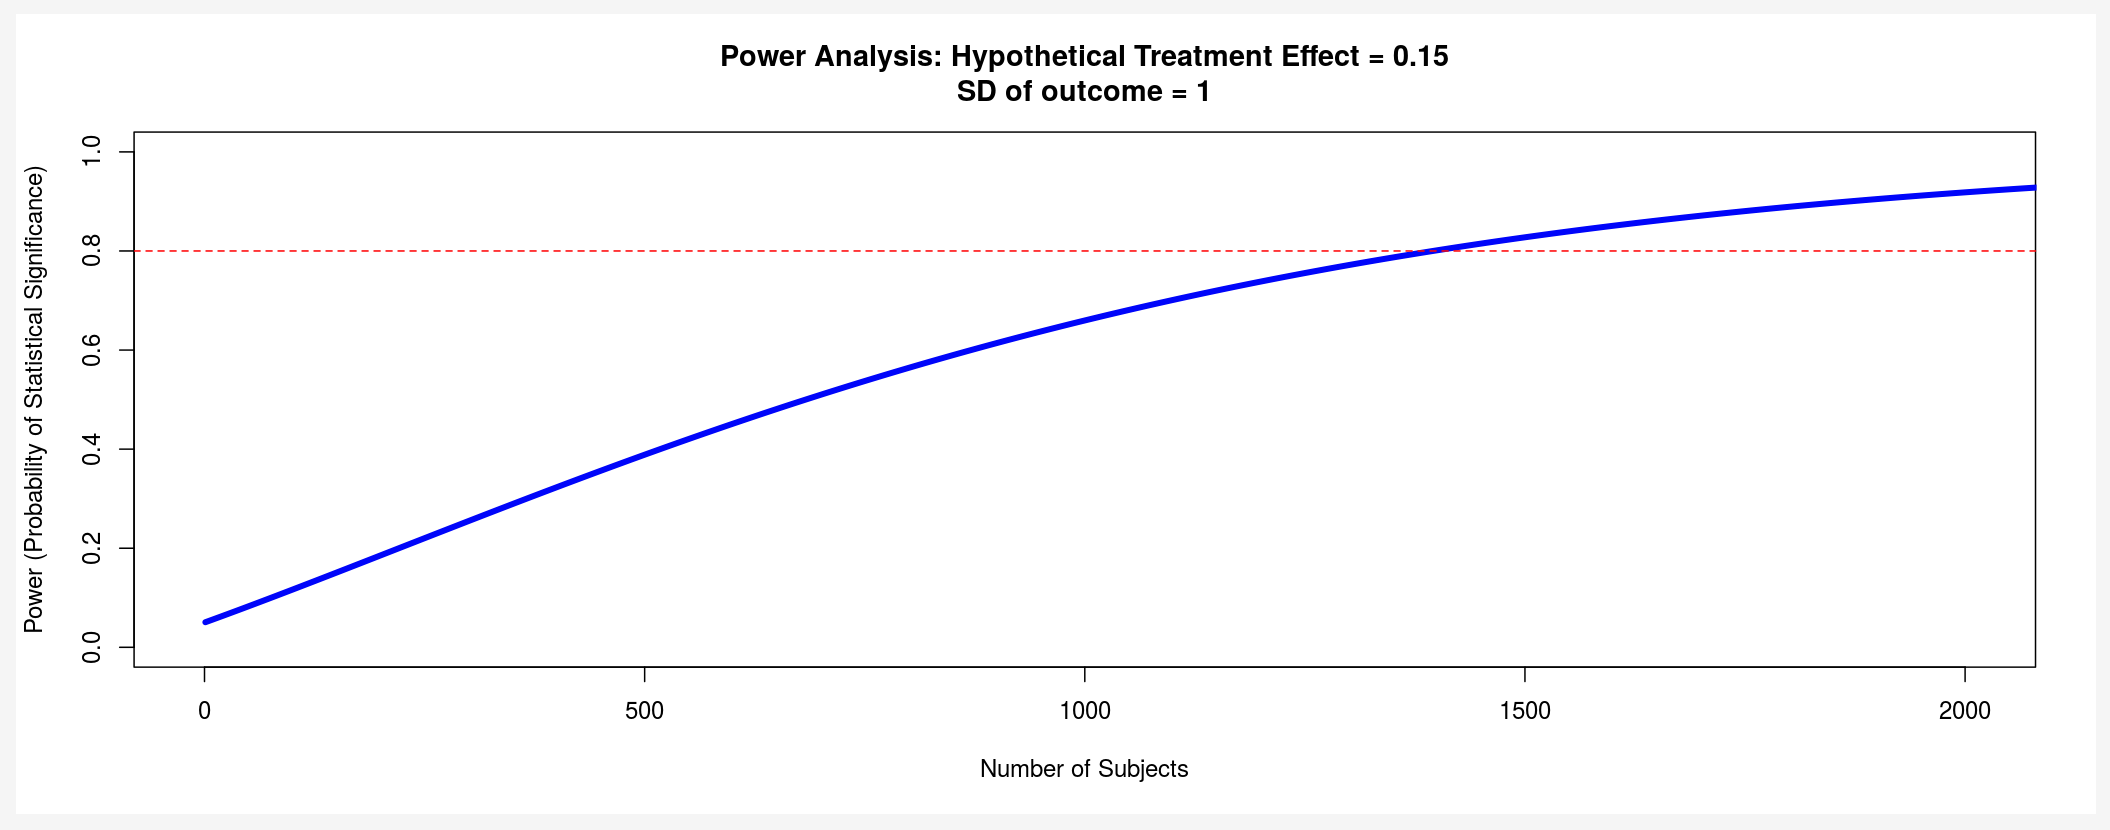
\includegraphics[width=13cm]{Images/pc_15.png}
        %\caption{Muestra necesaria para observar efectos de 0.15d.e con 80\% de poder}
    \end{subfigure}
    \begin{subfigure}{\textwidth} 
        \centering
        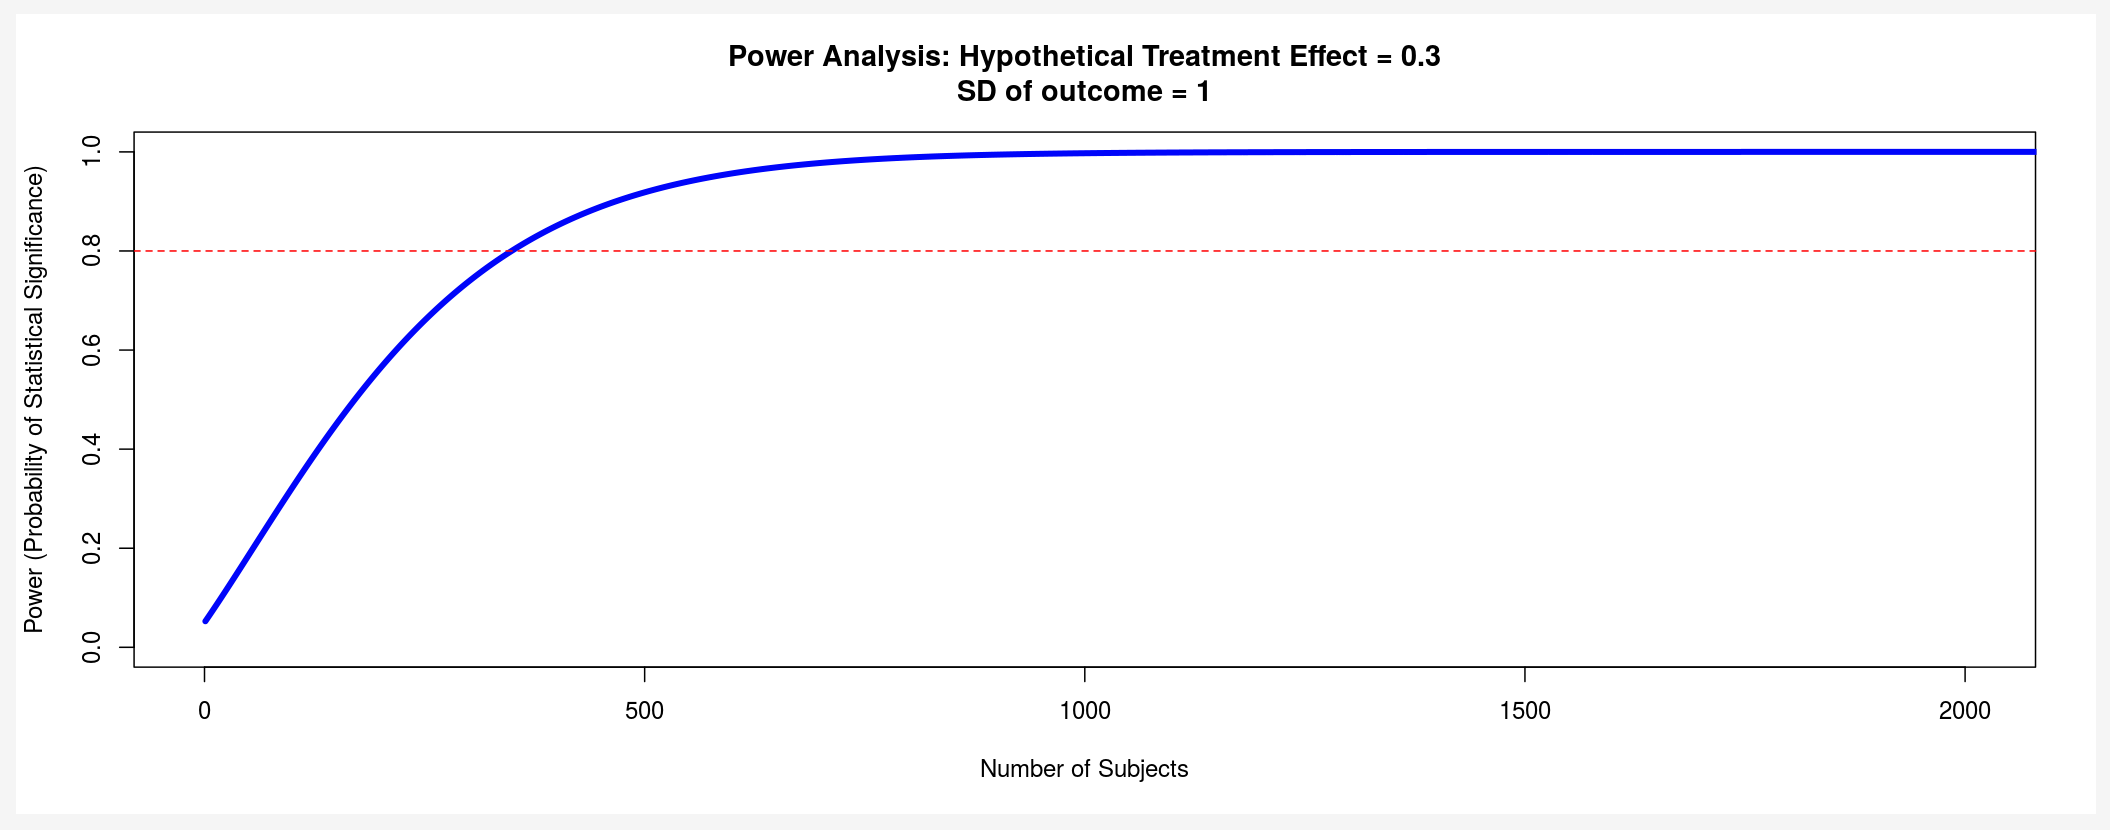
\includegraphics[width=13cm]{Images/pc_30.png}
        %\caption{Muestra necesaria para observar efectos de 0.3d.e con 80\% de poder}
    \end{subfigure}
    \label{fig:calc}
    \begin{singlespace}
        \floatfoot{\footnotesize{\textbf{Fuente:} Egap Power Tool }\par}
    \end{singlespace}
\end{figure}

    \vfill
    \pagebreak    
    %\section{Proceso de solución juego de señalización}
A continuación se evalúan los candidatos a equilibrio y se determina las condiciones para que sean equilibrios.  En caso de que el jugador 2 sea indiferente entre interactuar o no interactuar, se toma como mejor respuesta interactuar. Sea $\gamma_i$ la estrategia del jugador $i$, y $\forall k \in \{F,M\} $,
\small{
\begin{enumerate}
    % Agrupadores
    \item $\gamma_1(K)=E_k, \ \gamma_1(-K)=E_k, \ \gamma_1(O)=E_k$ %1%
    \begin{enumerate}
        \item Pagos esperados del Jugador 2
        \begin{enumerate}
            \item Creencias
                \begin{eqnarray*}
                    P(K|E_k)&=&\frac{P(E_k|K)P(K)}{P(E_k|F)P(K)+P(E_k|-K)P(-K)+P(E_k|O)P(O)}\\
                            &=&\frac{0.495}{0.495+0.495+0.01}\\
                            &=&0.495\\
                    P(-K|E_k)&=&\frac{P(E_k|-K)P(-K)}{P(E_k|F)P(K)+P(E_k|-K)P(-K)+P(E_k|O)P(O)}\\
                             &=&\frac{0.495}{0.495+0.495+0.01}\\
                             &=&0.495\\
                    P(O|E_k)&=&\frac{P(E_k|O)P(O)}{P(E_k|K)P(K)+P(E_k|-K)P(-K)+P(E_k|O)P(O)}\\
                            &=&\frac{0.01}{0.495+0.495+0.01}\\
                            &=&0.01\\
                    P(K|E_{-k})&=&p\\
                    P(-K|E_{-k})&=&q\\
                    P(O|E_{-k})&=&1-p-q\\
                \end{eqnarray*}

            \item Pagos esperados del Jugador 2
            \begin{itemize}
                \item Si el jugador 2 recibe $E_k$ como señal
                \begin{eqnarray*}
                U_{2}^{e}(I)&=&P(K|E_k)V(K,E_k,I)\ +\ P(-K|E_k)V(-K,E_k,I)\\
                            &+&P(O|E_k)V(O,E_k,I)\\
                            &=&0.495*0\ +\ 0.495*(-\theta)\ + \ 0.01*(-\theta)\\
                            &=&0.505*(-\theta)\\
                U_{2}^{e}(NI)&=&P(K|E_k)V(F,E_k,NI)\ +\ P(-K|E_k)V(-K,E_k,NI)\\
                             &+&P(O|E_k)V(O,E_k,NI)\\
                             &=&0.495*(-\eta)\ +\ 0.495*(-\eta)\ + \ 0.01*(-\eta)\\
                             &=&-\eta\\
                \end{eqnarray*}

                La mejor respuesta del jugador 2 si recibe un señal $E_k$ es:
                \begin{equation*}
                \gamma_2(E_k)=
                \begin{cases}
                    I \text{ si } \eta \geq 0.505\theta \\
                    NI \text{ si } \eta < 0.505\theta \\
                \end{cases}    
                \end{equation*}
                
                \item Si el jugador 2 recibe $E_{-k}$ como señal
                \begin{eqnarray*}
                U_{2}^{e}(I)&=&P(K|E_{-k})V(K,E_{-k},I)\ +\ P(-K|E_{-k})V(-K,E_{-k},I)\\
                            &+&P(O|E_{-k})V(O,E_{-k},I)\\
                            &=&p*(-\theta)\ +\ q*0\ + \ (1-p-q)*(-\theta)\\
                            &=&(1-q)*(-\theta)\\
                U_{2}^{e}(NI)&=&P(K|E_{-k})V(K,E_{-k},NI)\ +\ P(-K|E_m)V(-K,E_{-k},NI)\\ 
                             &+&P(O|E_{-k})V(O,E_{-k},NI)\\
                             &=&p*(-\eta)\ +\ q*(-\eta)\ + \ (1-p-q)*(-\eta)\\
                             &=&-\eta\\
                \end{eqnarray*}

                La mejor respuesta del jugador 2 si recibe un señal $E_{-k}$ es:
                \begin{equation*}
                \gamma_2(E_{-k})=
                \begin{cases}
                    I \text{ si } \eta \geq (1-q)\theta \\
                    NI \text{ si } \eta < (1-q)\theta \\
                \end{cases}    
                \end{equation*}
        \end{itemize}
        \end{enumerate}
        \item Incentivos a desviar del Jugador 1
        \begin{itemize}
        \item Si $\eta \in [0.505\theta,\infty) \wedge \eta \in [(1-q)\theta,\infty)$
            \begin{itemize}
                \item Si $ \iota_1=K  $, el jugador 1 no tiene incentivos a desviar si $ \Pi_k \geq \Pi_{-k} - \xi $
                \item Si $ \iota_1=-K $, el jugador 1 no tiene incentivos a desviar si $ \Pi_k - \xi \geq \Pi_{-k} $
                \item Si $ \iota_1=O  $, el jugador 1 no tiene incentivos a desviar si $ \Pi_k \geq \Pi_{-k} $
            \end{itemize}
        \item Si $\eta \in [0.505\theta,\infty) \wedge \eta \in (0,(1-q)\theta)$
            \begin{itemize}
                \item Si $ \iota_1=K  $, el jugador 1 no tiene incentivos a desviar si $ \Pi_k \geq \Pi_{-k} - \xi - \beta $
                \item Si $ \iota_1=-K $, el jugador 1 no tiene incentivos a desviar si $ \Pi_k - \xi \geq \Pi_{-k} - \beta $
                \item Si $ \iota_1=O  $, el jugador 1 no tiene incentivos a desviar si $ \Pi_k \geq \Pi_{-k} - \beta $
            \end{itemize}
        \item Si $\eta \in (0,0.505\theta) \wedge \eta \in [(1-q)\theta,\infty)$
            \begin{itemize}
                \item Si $ \iota_1=K  $, el jugador 1 no tiene incentivos a desviar si $ \Pi_k - \beta \geq \Pi_{-k} - \xi $
                \item Si $ \iota_1=-K $, el jugador 1 no tiene incentivos a desviar si $ \Pi_k - \xi - \beta \geq \Pi_{-k} $
                \item Si $ \iota_1=O  $, el jugador 1 no tiene incentivos a desviar si $ \Pi_k - \beta \geq \Pi_{-k} $
            \end{itemize}
        \item Si $\eta \in (0,0.505\theta) \wedge \eta \in (0,(1-q)\theta)$
            \begin{itemize}
                \item Si $ \iota_1=K  $, el jugador 1 no tiene incentivos a desviar si $ \Pi_k \geq \Pi_{-k} - \xi $
                \item Si $ \iota_1=-K $, el jugador 1 no tiene incentivos a desviar si $ \Pi_k - \xi \geq \Pi_{-k} $
                \item Si $ \iota_1=O  $, el jugador 1 no tiene incentivos a desviar si $ \Pi_k \geq \Pi_{-k} $
            \end{itemize}
        \end{itemize}
    
    Por lo tanto, 
    
    \noindent (i) $(\gamma_1(K)=\gamma_1(-K)=\gamma_1(O)=E_k, \gamma_2(E_k)=I, \gamma_2(E_{-k})=I)$ es equilibrio si $\eta \in [0.505\theta, \infty) \wedge \eta \in [(1-q)\theta, \infty) \wedge \Pi_1(E_{k})- \xi \geq \Pi_1(E_{-k})$ 
    
    \noindent (ii) $(\gamma_1(K)=\gamma_1(-K)=\gamma_1(O)=E_k, \gamma_2(E_k)=I, \gamma_2(E_{-k})=NI)$ es equilibrio si $\eta \in [0.505\theta, \infty) \wedge \eta \in (0, (1-q)\theta) \wedge \Pi_1(E_{k})- \xi \geq \Pi_1(E_{-k}-\beta)$ 
    
    \noindent (iii) $(\gamma_1(K)=\gamma_1(-K)=\gamma_1(O)=E_k, \gamma_2(E_k)=NI, \gamma_2(E_{-k})=I)$ es equilibrio si $\eta \in (0, 0.505\theta) \wedge \eta \in [(1-q)\theta, \infty) \wedge \Pi_1(E_{k})- \xi -\beta \geq \Pi_1(E_{-k})$ 
    
    \noindent (iv) $(\gamma_1(K)=\gamma_1(-K)=\gamma_1(O)=E_k, \gamma_2(E_k)=NI, \gamma_2(E_{-k})=NI)$ es equilibrio si $\eta\in (0, 0.505\theta) \wedge \eta \in (0, (1-q)\theta) \wedge \Pi_1(E_{k})- \xi \geq \Pi_1(E_{-k})$
    \end{enumerate}   
    
    % Separadores
    \item $\gamma_1(K)=E_k, \ \gamma_1(-K)=E_{-k}, \ \gamma_1(O)=E_{k}$ %2%
    \begin{enumerate}
    \item Pagos esperados del Jugador 2
    \begin{enumerate}
        \item Creencias
            \begin{eqnarray*}
                P(K|E_k)&=&\frac{P(E_k|K)P(K)}{P(E_k|K)P(K)+P(E_k|-K)P(-K)+P(E_k|O)P(O)}\\
                        &=&\frac{0.495}{0.495+0+0.01}\\
                        &=&0.98\\
                P(-K|E_k)&=&\frac{P(E_k|-K)P(-K)}{P(E_k|K)P(K)+P(E_k|-K)P(-K)+P(E_k|O)P(O)}\\
                        &=&\frac{0}{0.495+0+0.01}\\
                        &=&0\\
                P(O|E_k)&=&\frac{P(E_k|O)P(O)}{P(E_k|F)P(K)+P(E_k|-K)P(-K)+P(E_k|O)P(O)}\\
                        &=&\frac{0.01}{0.495+0+0.01}\\
                        &=&0.02\\
                P(K|E_{-k})&=&\frac{P(E_{-k}|F)P(K)}{P(E_{-k}|K)P(K)+P(E_{-k}|-K)P(-K)+P(E_{-k}|O)P(O)}\\
                        &=&\frac{0}{0+0.495+0}\\
                        &=&0\\
                P(-K|E_{-k})&=&\frac{P(E_{-k}|-K)P(-K)}{P(E_{-k}|K)P(K)+P(E_{-k}|-K)P(-K)+P(E_{-k}|O)P(O)}\\
                        &=&\frac{0.495}{0+0.495+0}\\
                        &=&1\\
                P(O|E_{-k})&=&\frac{P(E_{-k}|O)P(O)}{P(E_{-k}|K)P(K)+P(E_{-k}|-K)P(-K)+P(E_{-k}|O)P(O)}\\
                        &=&\frac{0}{0+0.495+0}\\
                        &=&0
            \end{eqnarray*}
        \item Pagos esperados del Jugador 2
        \begin{itemize}
           \item Si el jugador 2 recibe $E_k$ como señal
            \begin{eqnarray*}
                U_{2}^{e}(I)&=&P(K|E_k)V(K,E_k,I)\ +\ P(-K|E_k)V(-K,E_k,I)\\
                            &+&P(O|E_k)V(O,E_k,I)\\
                            &=&0.98*0\ +\ 0*(-\theta)\ + \ 0.02*(-\theta)\\
                            &=&0.02*(-\theta)\\
                U_{2}^{e}(NI)&=&P(K|E_k)V(K,E_k,NI)\ +\ P(-K|E_k)V(-K,E_k,NI)\\ 
                             &+&P(O|E_k)V(O,E_k,NI)\\
                             &=&0.98*(-\eta)\ +\ 0*(-\eta)\ + \ 0.02*(-\eta)\\
                             &=&-\eta
            \end{eqnarray*}

            La mejor respuesta del jugador 2 si recibe un señal $E_k$ es:
            \begin{equation*}
                \gamma_2(E_k)=
                \begin{cases}
                    I \text{ si } \eta \geq 0.02\theta \\
                    NI \text{ si } \eta < 0.02\theta \\
                \end{cases}    
               \end{equation*}
                
        \item Si el jugador 2 recibe $E_{-k}$ como señal
            \begin{eqnarray*}
                U_{2}^{e}(I)&=&P(K|E_{-k})V(K,E_{-k},I)\ +\ P(-K|E_{-k})V(-K,E_{-k},I)\\ 
                            &+&P(O|E_{-k})V(O,E_{-k},I)\\
                            &=&0*(-\theta)\ +\ 1*0\ + \ 0*(-\theta)\\
                            &=&0\\
                U_{2}^{e}(NI)&=&P(K|E_{-k})V(K,E_{-k},NI)\ +\ P(-K|E_{-k})V(-K,E_{-k},NI)\\
                             &+&P(O|E_{-k})V(O,E_{-k},NI)\\
                             &=&0*(-\eta)\ +\ 1*(-\eta)\ + \ 0*(-\eta)\\
                             &=&-\eta
            \end{eqnarray*}

            La mejor respuesta del jugador 2 (dado que $\eta>0$) si recibe un señal $E_{-k}$ es:
            \begin{equation*}
                \gamma_2(E_{-k})= I
            \end{equation*}
        \end{itemize}
        \end{enumerate}
        \item Incentivos a desviar del Jugador 1
        \begin{itemize}
        \item Si $\eta \in [0.02\theta,\infty) $
            \begin{itemize}
                \item Si $ \iota_1=K  $, el jugador 1 no tiene incentivos a desviar si $ \Pi_k \geq \Pi_{-k} - \xi $
                \item Si $ \iota_1=-K $, el jugador 1 no tiene incentivos a desviar si $ \Pi_{-k} \geq \Pi_{-k} - \xi $
                \item Si $ \iota_1=O  $, el jugador 1 no tiene incentivos a desviar si $ \Pi_k \geq \Pi_{-k} $
            \end{itemize}
        \item Si $\eta \in (0,0.02\theta) $
            \begin{itemize}
                \item Si $ \iota_1=K  $, el jugador 1 no tiene incentivos a desviar si $ \Pi_k \geq \Pi_{-k} - \xi - \beta $
                \item Si $ \iota_1=-K $, el jugador 1 no tiene incentivos a desviar si $ \Pi_{-k} -\beta \geq \Pi_{k} - \xi $
                \item Si $ \iota_1=O  $, el jugador 1 no tiene incentivos a desviar si $ \Pi_k - \beta \geq \Pi_{-k} $
            \end{itemize}
        \end{itemize}
    
    Por lo tanto, 

    \noindent (i) $(\gamma_1(K)=E_k, \gamma_1(-K)=E_{-k}, \gamma_1(O)=E_k, \gamma_2(E_k)=NI, \gamma_2(E_{-k})=I)$ es equilibrio si $\eta\in(0, 0.02\theta) \wedge \Pi_1(E_{k})- \beta \geq \Pi_1(E_{-k}) \geq  \Pi_1(E_{k})- \beta - \xi$

    \noindent (ii) $(\gamma_1(K)=E_k, \gamma_1(-K)=E_{-k}, \gamma_1(O)=E_k, \gamma_2(E_k)=I, \gamma_2(E_{-k})=I)$ es equilibrio si $\eta\in[0.02\theta, \infty) \wedge \Pi_1(E_{k}) \geq \Pi_1(E_{-k}) \geq \Pi_1(E_{k})- \xi$
    \end{enumerate}   

    \item $\gamma_1(K)=E_{-k}, \ \gamma_1(-K)=E_k, \ \gamma_1(O)=E_{k}$ %3%
    \begin{enumerate}
    \item Pagos esperados del Jugador 2
    \begin{enumerate}
        \item Creencias
            \begin{eqnarray*}
                P(K|E_k)&=&\frac{P(E_k|K)P(K)}{P(E_k|K)P(K)+P(E_k|-K)P(-K)+P(E_k|O)P(O)}\\
                        &=&\frac{0}{0+0.495+0}\\
                        &=&0\\
                P(-K|E_k)&=&\frac{P(E_k|-K)P(-K)}{P(E_k|K)P(K)+P(E_k|-K)P(-K)+P(E_k|O)P(O)}\\
                        &=&\frac{0.495}{0+0.495+0}\\
                        &=&1\\
                P(O|E_k)&=&\frac{P(E_k|O)P(O)}{P(E_k|K)P(K)+P(E_k|-K)P(-K)+P(E_k|O)P(O)}\\
                        &=&\frac{0.01}{0+0.495+0}\\
                        &=&0\\
                P(K|E_{-k})&=&\frac{P(E_{-k}|K)P(K)}{P(E_{-k}|K)P(K)+P(E_{-k}|-K)P(-K)+P(E_{-k}|O)P(O)}\\
                        &=&\frac{0.495}{0.495+0+0.01}\\
                        &=&0.98\\
                P(-K|E_{-k})&=&\frac{P(E_{-k}|-K)P(-K)}{P(E_{-k}|K)P(K)+P(E_{-k}|-K)P(-K)+P(E_{-k}|O)P(O)}\\
                        &=&\frac{0}{0.495+0+0.01}\\
                        &=&0\\
                P(O|E_{-k})&=&\frac{P(E_{-k}|O)P(O)}{P(E_{-k}|K)P(K)+P(E_{-k}|-K)P(-K)+P(E_{-k}|O)P(O)}\\
                        &=&\frac{0.01}{0.495+0+0.01}\\
                        &=&0.02
            \end{eqnarray*}
            
        \item Pagos esperados del Jugador 2
        \begin{itemize}
            \item Si el jugador 2 recibe $E_k$ como señal
            \begin{eqnarray*}
                U_{2}^{e}(I)&=&P(K|E_k)V(K,E_k,I)\ +\ P(-K|E_k)V(-K,E_k,I)\\ 
                            &+&P(O|E_k)V(O,E_k,I)\\
                            &=&0*0\ +\ 1*(-\theta)\ + \ 0*(-\theta)\\
                            &=&-\theta\\
                U_{2}^{e}(NI)&=&P(K|E_k)V(K,E_k,NI)\ +\ P(-K|E_k)V(-K,E_k,NI)\\ 
                             &+&P(O|E_k)V(O,E_kNI)\\
                             &=&0*(-\eta)\ +\ 1*(-\eta)\ + \ 0*(-\eta)\\
                             &=&-\eta
            \end{eqnarray*}

            La mejor respuesta del jugador 2 si recibe un señal $E_k$ es:
            \begin{equation*}
                \gamma_2(E_k)=
                \begin{cases}
                    I \text{ si } \eta \geq \theta \\
                    NI \text{ si } \eta < \theta \\
                \end{cases}    
            \end{equation*}
                
        \item Si el jugador 2 recibe $E_{-k}$ como señal
            \begin{eqnarray*}
                U_{2}^{e}(I)&=&P(K|E_{-k})V(K,E_{-k},I)\ +\ P(-K|E_{-k})V(-K,E_{-k},I)\\ 
                            &+&P(O|E_{-k})V(O,E_{-k},I)\\
                            &=&0.98*(-\theta)\ +\ 0*0\ + \ 0.02*(-\theta)\\
                            &=&-\theta
            \end{eqnarray*}
            \begin{eqnarray*}
                U_{2}^{e}(NI)&=&P(K|E_{-k})V(K,E_{-k},NI)\ +\ P(-K|E_{-k})V(-K,E_{-k},NI)\\
                             &+&P(O|E_{-k})V(O,E_{-k},NI)\\
                             &=&0.98*(-\eta)\ +\ 0*(-\eta)\ + \ 0.02*(-\eta)\\
                             &=&-\eta
            \end{eqnarray*}
            La mejor respuesta del jugador 2 si recibe un señal $E_{-k}$ es:
            \begin{equation*}
                \gamma_2(E_{-k})=
                \begin{cases}
                    I \text{ si } \eta \geq \theta \\
                    NI \text{ si } \eta < \theta \\
                \end{cases}    
            \end{equation*}
        \end{itemize}
    \end{enumerate}
    \item Incentivos a desviar del Jugador 1
    \begin{itemize}
        \item Si $\eta \in [\theta,\infty) $
            \begin{itemize}
                \item Si $ \iota_1=K  $, el jugador 1 no tiene incentivos a desviar si $ \Pi_{-k} - \xi \geq \Pi_k $
                \item Si $ \iota_1=-K $, el jugador 1 no tiene incentivos a desviar si $ \Pi_k - \xi \geq \Pi_{-k} $
                \item Si $ \iota_1=O  $, el jugador 1 no tiene incentivos a desviar si $ \Pi_k \geq \Pi_{-k} $
            \end{itemize}
        \item Si $\eta \in (0,\theta) $
            \begin{itemize}
                \item Si $ \iota_1=K  $, el jugador 1 no tiene incentivos a desviar si $ \Pi_{-k} - \xi \geq \Pi_k $
                \item Si $ \iota_1=-K $, el jugador 1 no tiene incentivos a desviar si $ \Pi_k - \xi \geq \Pi_{-k} $
                \item Si $ \iota_1=O  $, el jugador 1 no tiene incentivos a desviar si $ \Pi_k \geq \Pi_{-k} $
        \end{itemize}
    \end{itemize}
    
    Por lo tanto, no hay equilibrio si $\gamma_1(K)=E_{-k}, \ \gamma_1(-K)=E_k, \ \gamma_1(O)=E_{k}$
    \end{enumerate}
       
    \item $\gamma_1(K)=E_k, \ \gamma_1(-K)=E_k, \ \gamma_1(O)=E_{-k}$ %4%
    \begin{enumerate}
    \item Pagos esperados del Jugador 2
    \begin{enumerate}
        \item Creencias
            \begin{eqnarray*}
                P(K|E_k)&=&\frac{P(E_k|K)P(K)}{P(E_k|K)P(K)+P(E_k|-K)P(-K)+P(E_k|O)P(O)}\\
                        &=&\frac{0.495}{0.495+0.495+0}\\
                        &=&0.5\\
                P(-K|E_k)&=&\frac{P(E_k|-K)P(-K)}{P(E_k|K)P(K)+P(E_k|-K)P(-K)+P(E_k|O)P(O)}\\
                        &=&\frac{0.495}{0.495+0.495+0}\\
                        &=&0.5\\
                P(O|E_k)&=&\frac{P(E_k|O)P(O)}{P(E_k|K)P(K)+P(E_k|-K)P(-K)+P(E_k|O)P(O)}\\
                        &=&\frac{0}{0.495+0.495+0}\\
                        &=&0\\
                P(K|E_{-k})&=&\frac{P(E_{-k}|K)P(K)}{P(E_{-k}|K)P(K)+P(E_{-k}|-K)P(-K)+P(E_{-k}|O)P(O)}\\
                        &=&\frac{0}{0+0+0.01}\\
                        &=&0\\
                P(-K|E_{-k})&=&\frac{P(E_{-k}|-K)P(-K)}{P(E_{-k}|K)P(K)+P(E_{-k}|-K)P(-K)+P(E_{-k}|O)P(O)}\\
                        &=&\frac{0}{0+0+0.1}\\
                        &=&0\\
                P(O|E_{-k})&=&\frac{P(E_{-k}|O)P(O)}{P(E_{-k}|K)P(K)+P(E_{-k}|-K)P(-K)+P(E_{-k}|O)P(O)}\\
                        &=&\frac{0.1}{0+0+0.1}\\
                        &=&1
            \end{eqnarray*}
        \item Pagos esperados del Jugador 2
        \begin{itemize}
        \item Si el jugador 2 recibe $E_k$ como señal
            \begin{eqnarray*}
                U_{2}^{e}(I)&=&P(K|E_k)V(K,E_k,I)\ +\ P(-K|E_k)V(-K,E_k,I)\\
                            &+&P(O|E_k)V(O,E_k,I)\\
                            &=&0.5*0\ +\ 0.5*(-\theta)\ + \ 0*(-\theta)\\
                            &=&0.5*(-\theta)\\
                U_{2}^{e}(NI)&=&P(K|E_k)V(K,E_k,NI)\ +\ P(-K|E_k)V(-K,E_k,NI)\\ 
                             &+&P(O|E_k)V(O,E_k,NI)\\
                             &=&0.5*(-\eta)\ +\ 0.5*(-\eta)\ + \ 0*(-\eta)\\
                             &=&-\eta
            \end{eqnarray*}

            La mejor respuesta del jugador 2 si recibe un señal $E_k$ es:
            \begin{equation*}
                \gamma_2(E_k)=
                \begin{cases}
                    I \text{ si } \eta \geq 0.5\theta \\
                    NI \text{ si } \eta < 0.5\theta \\
                \end{cases}    
            \end{equation*}
                
        \item Si el jugador 2 recibe $E_{-k}$ como señal
            \begin{eqnarray*}
                U_{2}^{e}(I)&=&P(K|E_{-k})V(K,E_{-k},I)\ +\ P(-K|E_{-k})V(K,E_{-k},I)\\
                            &+&P(O|E_{-k})V(O,E_{-k},I)\\
                            &=&0*(-\theta)\ +\ 0*0\ + \ 1*(-\theta)\\
                            &=&-\theta\\
                U_{2}^{e}(NI)&=&P(K|E_{-k})V(K,E_{-k},NI)\ +\ P(-K|E_{-k})V(-K,E_{-k},NI)\\
                             &+&P(O|E_{-k})V(O,E_{-k},NI)\\
                             &=&0*(-\eta)\ +\ 0*(-\eta)\ + \ 1*(-\eta)\\
                             &=&-\eta
            \end{eqnarray*}

            La mejor respuesta del jugador 2 si recibe un señal $E_{-k}$ es:
            \begin{equation*}
                \gamma_2(E_{-k})=
                \begin{cases}
                    I \text{ si } \eta \geq \theta \\
                    NI \text{ si } \eta < \theta \\
                \end{cases}    
            \end{equation*}
        \end{itemize}
    \end{enumerate}
    \item Incentivos a desviar del Jugador 1
    \begin{itemize}
        \item Si $\eta \in [\theta,\infty) $
            \begin{itemize}
                \item Si $ \iota_1=K  $, el jugador 1 no tiene incentivos a desviar si $ \Pi_k \geq \Pi_{-k} - \xi $
                \item Si $ \iota_1=-K $, el jugador 1 no tiene incentivos a desviar si $ \Pi_k - \xi \geq \Pi_{-k} $
                \item Si $ \iota_1=O  $, el jugador 1 no tiene incentivos a desviar si $ \Pi_k \geq \Pi_{-k} $
            \end{itemize}
        \item Si $\eta \in [0.5\theta, \theta) $
            \begin{itemize}
                \item Si $ \iota_1=K  $, el jugador 1 no tiene incentivos a desviar si $ \Pi_k \geq \Pi_{-k} - \xi - \beta $
                \item Si $ \iota_1=-K $, el jugador 1 no tiene incentivos a desviar si $ \Pi_k - \xi \geq \Pi_{-k} - \beta $
                \item Si $ \iota_1=O  $, el jugador 1 no tiene incentivos a desviar si $ \Pi_{-k} - \beta \geq \Pi_{k} $
            \end{itemize}
        \item Si $\eta \in (0, 0.5\theta) $
            \begin{itemize}
                \item Si $ \iota_1=K  $, el jugador 1 no tiene incentivos a desviar si $ \Pi_k \geq \Pi_{-k} - \xi $
                \item Si $ \iota_1=-K $, el jugador 1 no tiene incentivos a desviar si $ \Pi_k - \xi \geq \Pi_{-k} $
                \item Si $ \iota_1=O  $, el jugador 1 no tiene incentivos a desviar si $ \Pi_k \geq \Pi_{-k} $
            \end{itemize}
    \end{itemize}
    
    Por lo tanto, no hay equilibrio si $\gamma_1(K)=E_k, \ \gamma_1(-K)=E_k, \ \gamma_1(O)=E_{-k}$.
    \end{enumerate}
  
    
\end{enumerate}
}



    \vfill
    \pagebreak 
    %\section{Protocolo experimental}
\subsection{Inscripción y Encuesta}
\textit{Dos semanas: del 20 al 31 de enero.\\
Reclutamiento con afiches, volantes y a través de redes sociales.\\}
Agradecemos su participación en este ejercicio que hace parte de un estudio sobre decisiones individuales y bienestar universitario. Usted podrá ganar hasta \$70.000 pesos dependiendo de las decisiones que tomen usted y otras personas de la universidad. Usted puede retirarse en cualquier momento. Pero, solamente si completa el ejercicio, recibirá la cantidad de dinero que gane por su desempeño. \\
El dinero utilizado para pagarle a los participantes ha sido aportado por financiadores externos al estudio.\\

Este ejercicio consiste en un concurso de memes sobre bienestar universitario. Los memes deben comunicar un problema o una solución a un problema de bienestar universitario y deben ser desarrollados en grupos de tres personas. Un panel de jurados\footnote{El panel de jurados está conformado por profesores y asistentes de investigación de la Facultad de Economía de la Universidad de los Andes.} elegirá los 7 mejores memes y los investigadores entregarán los premios correspondientes a los grupos que hayan presentado esos memes. Los premios son:

\begin{itemize}
    \item Primer puesto \$210.000
    \item Segundo puesto \$180.000
    \item Tercer puesto \$150.000
    \item Cuarto puesto \$120.000
    \item Quinto puesto \$90.000
    \item Sexto puesto \$60.000
    \item Séptimo puesto \$30.000
\end{itemize}
El concurso tiene tres partes: inscripción, conformación de grupos y desarrollo de memes.\footnote{La inscripción está abierta del 20 al 31 de enero. Los grupos se conformarán del 3 al 7 de febrero y los memes se desarrollarán del 10 al 20 de febrero. El 28 de febrero se anuncian los ganadores.}\\
A continuación, le vamos a explicar cómo se conforman los grupos. \textbf{Por favor lea con atención las siguientes instrucciones.}\\
Los grupos se determinarán siguiendo el siguiente proceso:
\begin{itemize}
    \item Los investigadores conformarán secciones de 9 personas para formar 3 grupos de 3 personas.
    \item Usted observará una tarjeta con características generales para cada una de las otras 8 personas de su sección.
    \item Usted deberá organizar esas 8 tarjetas en el orden en el que quiere que hagan parte de su grupo.
    \begin{itemize}
        \item La persona con la que más le gustaría desarrollar el meme, debería ponerla en el primer lugar.
        \item La segunda persona con la que usted más le gustaría desarrollar el meme, debería ponerla en el segundo lugar.
        \item De tal manera que, la persona con la que menos le gustaría desarrollar el meme, debería ponerla en el último lugar.
    \end{itemize}
\end{itemize}
\textit{Grupo 1}
\begin{itemize}
    \item Luego de recibir todas las listas, los investigadores elegirán al azar a una de las nueve personas de la sección. Llamemos esa persona, la persona A.
    \item El grupo 1 será conformado por la persona A y las dos primeras personas en la lista de la persona A.
\end{itemize}
\textit{Grupo 2}
\begin{itemize}
    \item De las seis personas que no fueron asignadas al grupo 1, los investigadores elegirá una persona al azar. Llamemos a esa persona, la persona B.
    \item El segundo grupo será conformado por la persona B y las dos personas que ocupen los primeros puestos de la lista de la persona B (que no hayan sido asignados al grupo 1).
\end{itemize}
\textit{Grupo 3}
\begin{itemize}
    \item El tercer grupo será conformado por las tres personas que no fueron asignadas ni al grupo 1, ni al 2.
\end{itemize}
Para el desarrollo de esta actividad por favor respondan la siguiente encuesta que nos permitirá identificar cuáles son los temas de bienestar universitario que más le conciernen y conocer información básica suya.
Toda la información que usted brinde en este estudio es confidencial y será utilizada solamente con fines académicos. 
Ni su nombre, ni su identificación aparecerán en los informes o reportes de este estudio.\\
Dada esta información, queremos confirmar que usted desea participar en este estudio. Acceda al consentimiento informado 
\href{https://www.dropbox.com/s/2l9pwtj3sp1vbax/Consentimiento\%20Informado.pdf?dl=0}{acá}.\\

\pagebreak

\subsubsection{Encuesta de entrada}
\begin{enumerate}
\item Nombre y Apellido:
\item Correo Uniandes (incluya @uniandes.edu.co):
\item Género: (Femenino, Masculino, Otro)
\item Edad: (Min 18)
\item Departamento de nacimiento:
\item Programa principal: (lista)
\item Doble programa: (lista)
\item ¿Se ha cambiado de carrera?
\item ¿Cuántos semestres ha cursado? (Incluya el semeste que está cursando):
\item ¿Cuál es el nivel educativo más alto alcanzado por su madre? (lista)
\item ¿Cuál es el nivel educativo más alto alcanzado por su padre? (lista)
\item ¿Cuántos hermanos tiene? (Si no tiene hermanos, responda 0):
\item Seleccioné cuál de las siguientes vestimentas usaría usted con mayor frecuencia para ir a la universidad: (Imágenes de vestimentas, en orden aleatorio)
\item Para cada una de las siguientes, indique qué tan hábil es usted. Donde 1 indica no es hábil y 4 indica es fuertemente hábil.
\begin{enumerate}
    \item Comunicación (escucha, habla y escritura):
    \item Análisis e investigación:
    \item Adaptabilidad:
    \item Matemáticas:
    \item Tomar decisiones:
    \item Planeación:
    \item Hablar en público:
    \item Programación:
\end{enumerate}
\item Elija la opción que mejor describa sus habilidades
\begin{enumerate}
    \item Mucho más hábil en matemáticas | Algo más hábil en matemáticas | Algo más hábil comunicándose |  Mucho más hábil comunicándose
    \item Mucho más hábil adaptándose a diferentes escenarios | Algo más hábil adaptándose a diferentes escenarios | Algo más hábil en planeación | Mucho más hábil en planeación
\end{enumerate}
\item \textbf{Recuerde que este concurso de memes es sobre alguno de los siguientes problemas de bienestar universitario.} Para cada uno de los siguientes problemas de bienestar universitario indique el grado de importancia que usted les da. Donde 1 es no es importante y 4 es muy importante.
\begin{enumerate}
\item Carga académica:
\item Manejo de estrés por parte de los estudiantes:
\item Exclusión social:
\item Dificultad para expresar opiniones e ideas:
\item Falta de sentido:
\item Poca atención de los profesores a los estudiantes:
\item Falta de baños unificados
\item Soledad:
\item Dificultades económicas:
\item Exceso de competencia e individualismo entre estudiantes:
\item Plagio:
\item Falta de apoyo psicológico:
\item Excesiva atención a las notas:
\item Dificultades para trabajar en grupo:
\item Consumo de alcohol y drogas:
\end{enumerate}
\item Para cada una de las siguientes, indique de 1 a 4 qué tan importante es para usted tener \_\_\_\_\_\_\_ en los próximos 10 años. Donde 1 indica no es importante y 4 indica es esencial.
\begin{enumerate}
\item Estabilidad familiar
\item Una maestría
\item Un doctorado
\item Vivir muy cómodo económicamente
\item Reconocimiento público 
\item Vida espiritual
\item Bienestar físico
\end{enumerate}
\item Elija la opción que mejor describa sus aspiraciones para los próximos 10 años
\begin{enumerate}
    \item Aspira mucho más tener reconocimiento público | Aspira algo más tener reconocimiento público | Aspira algo más tener vida espiritual |  Aspira mucho más tener vida espiritual
    \item Aspira mucho más tener comodidad económica | Aspira algo más tener comodidad económica | Aspira algo más tener una familia estable	Aspira mucho más tener una familia estable
\end{enumerate}
\item ¿Ha contado con apoyo financiero durante su carrera?
\item Desde que entró a la universidad, ¿ha asistido a consejería académica o psicológica?
\end{enumerate}
Gracias por participar en este ejercicio, ha terminado la primera parte\\\
El 3 de febrero usted recibirá un correo para que pueda elegir sus grupo.


\subsection{Formación de grupos}
\textit{Una semanas: del 3 al 7 de febrero.\\
Contacto a través del correo. \\}
\fbox{
\begin{minipage}[t]{1\textwidth}
\textit{Nombre,}\\
Gracias por participar en el concurso de memes sobre bienestar universitario.\\
Para elegir el grupo con el que va a realizar el meme, por favor ingrese \textbf{desde un computador} al siguiente link: \textit{link votación}. Su identificador personal para entrar a esa página es \textit{(ID asignado)}.\\

Cordial saludo,\\
Equipo concurso bienestar universitario
\end{minipage}
}
\vspace*{0.5cm}\\ 
Agradecemos su participación en este ejercicio que hace parte de un estudio sobre decisiones individuales y bienestar universitario. Recuerde que usted podrá ganar hasta \$70.000 pesos dependiendo de las decisiones que tomen usted y otras personas de la universidad. Usted puede retirarse en cualquier momento. Pero, solamente si completa el ejercicio, recibirá la cantidad de dinero que gane por su desempeño.\\

\noindent\textbf{\Large{La siguiente parte únicamente se puede completar en computador. Por favor no responda desde un celular o tableta.}}\\
Los grupos se determinarán siguiendo el siguiente proceso:
\begin{itemize}
    \item Los investigadores conformarán secciones de 9 personas para formar 3 grupos de 3 personas.
    \item Usted observará una tarjeta con características generales para cada una de las otras 8 personas de su sección.
    \item Usted deberá organizar esas 8 tarjetas en el orden en el que quiere que hagan parte de su grupo.
    \begin{itemize}
        \item La persona con la que más le gustaría desarrollar el meme, debería ponerla en el primer lugar.
        \item La segunda persona con la que usted más le gustaría desarrollar el meme, debería ponerla en el segundo lugar.
        \item De tal manera que, la persona con la que menos le gustaría desarrollar el meme, debería ponerla en el último lugar.
    \end{itemize}
\end{itemize}
\textit{Grupo 1}
\begin{itemize}
    \item Luego de recibir todas las listas, los investigadores elegirán al azar a una de las nueve personas de la sección. Llamemos esa persona, la persona A.
    \item El grupo 1 será conformado por la persona A y las dos primeras personas en la lista de la persona A.
\end{itemize}
\textit{Grupo 2}
\begin{itemize}
    \item De las seis personas que no fueron asignadas al grupo 1, los investigadores elegirá una persona al azar. Llamemos a esa persona, la persona B.
    \item El segundo grupo será conformado por la persona B y las dos personas que ocupen los primeros puestos de la lista de la persona B (que no hayan sido asignados al grupo 1).
\end{itemize}
\textit{Grupo 3}
\begin{itemize}
    \item El tercer grupo será conformado por las tres personas que no fueron asignadas ni al grupo 1, ni al 2.
\end{itemize}
A continuación usted observará los ocho perfiles de las personas de su sección y deberá organizarlos según como quiere que participen de su grupo. \textbf{Recuerde que el orden de su lista determinará quién estará en su grupo.}\\
\textbf{Por favor ordene los siguientes perfiles en el orden en el que quiere que hagan parte de su grupo.\\
Recuerde que el orden de su lista determinará quién estará en su grupo.}\\
\textcolor{red}{Insertar screenshot de orden.}\\
Para los siguientes grupos, elija con cuál preferiría desarrollar el meme para este concurso. Se presenta 4 veces la siguiente decisión:\\
\textcolor{red}{Insertar screenshot de decisión.}\\
Gracias por participar en este ejercicio, ha terminado la segunda parte.\\
El 10 de febrero usted recibirá un correo para informarle quiénes están en su grupo y el correo para que los pueda contactar.

\subsection{Desarrollo de actividad}
Su identificador de grupo para este concurso es (ID asignado). 

Los miembros de este grupo son:
\begin{enumerate}
    \item Integrante 1. Correo
    \item Integrante 2. Correo
    \item Integrante 3. Correo
\end{enumerate}
En este grupo deben desarrollar un meme en el que se presente una descripción de uno de los siguiente problema de bienestar universitario y se proponga una solución:
\begin{enumerate}
\item 
\item 
\end{enumerate}

El vídeo debe ser enviado antes del \textbf{fecha a las 23:59}. 
El día \textit{8 días después de la fecha de entrega} se conocerán los dos grupos ganadores. 

\subsection{Encuesta de cierre}
Gracias por participar en el concurso. 
Hemos recibido su meme. Para que su meme sea tomado en cuenta por el panel de jurados, debe completar siguiente encuesta que no le tomará más de 10 minutos.  
Por último queremos pedirle que evalúe de 0 a 100 el desempeño de los demás miembros de su grupo ingresando al siguiente hipervínculo: 
El día \textit{8 días después de la fecha de entrega} se conocerán los dos grupos ganadores.





















\end{appendix}

\vfill
\pagebreak
\bibliographystyle{Ref/apalike-es}
\bibliography{Ref/ref}
\end{document}

